% Included Packages
\documentclass[12pt]{report}
\usepackage{aums}   
\usepackage{ulem}   
\usepackage{url}
\usepackage{tikz}
\usepackage{pgf}
\usepackage{tocloft}
\usepackage[intoc]{nomencl}
\usepackage[nottoc,notlof,notlot]{tocbibind}
\usepackage{times}
\usepackage[a4paper,left=1in,right=1in,top=1.15in,bottom=1in]{geometry}
\usepackage{etoolbox}
\usepackage{titlesec}
\usepackage[sorting=none]{biblatex}
\usepackage[final]{microtype}
\usepackage{booktabs}
\usepackage{xcolor}
\usepackage[T1]{fontenc}
\usepackage{amsmath}
\usepackage{indentfirst}
\usepackage{appendix}
\emergencystretch=1em

\addbibresource{Thesis.bib}
\setcounter{biburlnumpenalty}{9000}
\graphicspath{Figures/}

% Title Formatting
\titleformat{\chapter}[display] 
  {\singlespace\center}{\chaptertitlename\ \thechapter}{12pt}{\center} 
  \titleformat*{\section} {\normalfont\fontsize{12}{12}}  
\titleformat*{\subsection} {\normalfont\fontsize{12}{12}}
\titleformat*{\subsubsection} {\normalfont\fontsize{12}{12}}
\setlength\cftparskip{-2pt}

% Creating custom commands
\renewcommand\bibname{References}
\renewcommand\cftchapafterpnum{\vspace\baselineskip}  
\renewcommand\cftsecafterpnum{\vspace\baselineskip\normalfont}
\renewcommand\cftsubsecafterpnum{\vspace\baselineskip\normalfont}
\renewcommand\cftsubsubsecafterpnum{\vspace\baselineskip\normalsize}
\renewcommand\cftfigafterpnum{\vspace\baselineskip}
\renewcommand\cfttabafterpnum{\vspace\baselineskip}
\renewcommand{\cftpartleader}{\cftdotfill{\cftdotsep}}
\renewcommand{\cftchapleader}{\cftdotfill{\cftdotsep}}
\renewcommand{\nomname}{List of Abbreviations}


\makenomenclature{}



\newtheorem{theorem}{\normalfontTheorem} [chapter]

% Title 
\title{Deep Integration of a Flight Vehicle Dynamic Model in a Vector Tracking Software Defined Receiver}
\author{Noah S. Miller} 
\date{December 15}
\copyrightyear{2023}

\keywords{Simulation, GNSS/INS Integration, Aircraft Modeling}
 
\adviser{Scott M. Martin}

\professor{Scott M. Martin, Assistant Professor of Mechanical Engineering}

\professor{David M. Bevly, Bill and Lana McNair Distinguished Professor of Mechanical Engineering}

\professor{Chad G. Rose, Assistant Professor of Mechanical Engineering}

\begin{document}

\begin{romanpages}      % roman-numbered pages 

  \TitlePage{}
  \begin{abstract}
    % What is being presented in this work?
    As modern technology trends towards autonomous aerial and ground vehicles, the need for high-fidelity simulations is ever present. This thesis investigates the deep coupling of a high-fidelity Flight Vehicle Dynamic Model (FVDM) with simulated Global Positioning System (GPS) measurements in both healthy and degraded scenarios.
    % Why is it important?
    Aircraft in production today are equipped with a plethora of sensors that provide redundant global position of the flight vehicle. However, although redundant, these sensors are plagued with detrimental characteristics that inhibit high-precision measurements when used alone. Deeply coupling the measurements from these sensors with GPS correlators provides robust flight vehicle localization that is well-documented. But, the foreign threat to jam and degrade GPS signals is imminent, and new solutions that fuse multiple sensors must be evaluated when GPS is not available.
    % How is the sensor fusion algorithm going to work?
    This thesis presents a deeply fused sensor fusion algorithm that incorporates the FVDM and GPS correlator measurements. The sensor fusion algorithm will be tested in scenarios of GPS-degradation or GPS-denied environments. The FVDM and GPS correlator measurements are linked together through use of vector tracking, where the propagated states from the FVDM are used to predict the changes in carrier and code phase changes, helping the GPS receiver maintain signal lock are each of the acquired satellites.
    % What are the intricacies of the Flight Vehicle Dynamic Model?
    The FVDM is a high-fidelity flight vehicle model based on the Diamond DA-40 single-propeller fixed wing aircraft. The aircraft model simulates a piston engine model that generates thrust power through a shaft that spins a numerically modeled 5-blade propeller. The speed of the propeller is controlled through a electric governor, and the pitch is controlled to maintain efficient propeller action onto the incident airflow. The aerodynamics of the aircraft are modeled a discretized aerodynamic coefficient technique, called strip theory. Although not used in this work, a landing gear model incorporates the 3 landing gear seen on the Diamond DA-40 and evaluates the forces applied during landing as a second-order spring-mass-damper system. An International Standard Atmosphere (ISA) is used to calculate the density, temperature, speed of sound, and ambient pressure based on aircraft altitude. To close the loop of the FVDM, a set of controllers in collaboration with a waypoint manager are used to actuate the control surfaces on the aircraft. Multiple planned paths are demonstrated during this work and are presented in their respective sections.
    % Why use GPS measurements?
    For several decades, GPS has served as the backbone for attaining a global position solution on a variety of collection platforms. This ubiquity is well-documented, making GPS a practical and realistic signal to simulate for the focus of this thesis. Mainly used as medium to localize United States government entities, including the military services, means foreign threats are honing the technology needed to disrupt the GPS signal from jamming the signal-in-space to spoof the receiver by masking a GPS-like signal. These imminent threats catalyze the greater need for more research in this area on all collection platforms, including flight vehicles.
    % What results are shown in this thesis?
    This thesis investigates the performance of position estimation a simulated flight vehicle in scenarios of GPS-degradation and GPS-denied environments. Chapter 1 divulges prior art related to the investigation, while chapters 2, 3, and 4 describe the FVDM, GPS simulation and receiver architecture, and sensor fusion algorithm respectively. Chapter 5 presents the results, including a Monte-Carlo analysis of the stochastic elements within the simulations and Chapter 6 concludes the work followed by a section of future work for interested parties.
  \end{abstract}

  \begin{acknowledgments}
    Put text of the acknowledgments here.
  \end{acknowledgments}


  % Creating Table of Contents, List of Figures, List of Tables
  \begin{singlespace}

    \begin{center}
      \renewcommand{\cftchapfont}{}
      \renewcommand{\cftchappagefont}{}
      \renewcommand{\cfttoctitlefont}{\normalsize}% Remove \bfseries from ToC title
      \renewcommand{\cftsecfont}{\normalsize}% Remove \bfseries from section titles in ToC
      \renewcommand{\cftsecpagefont}{\normalsize}% Remove \bfseries from section titles' page in ToC
      \tableofcontents
      \newpage
      \renewcommand{\cftchapfont}{}
      \renewcommand{\cftchappagefont}{}
      \renewcommand{\cftloftitlefont}{\normalsize}% Remove \bfseries from lof title
      \renewcommand{\cftsecfont}{\normalsize}% Remove \bfseries from section titles in lof
      \renewcommand{\cftsecpagefont}{\normalsize}% Remove \bfseries from section titles' page in lof
      \listoffigures
      \newpage
      \renewcommand{\cftchapfont}{}
      \renewcommand{\cftchappagefont}{}
      \renewcommand{\cftlottitlefont}{\normalsize}% Remove \bfseries from lot title
      \renewcommand{\cftsecfont}{\normalsize}% Remove \bfseries from section titles in lof
      \renewcommand{\cftsecpagefont}{\normalsize}% Remove \bfseries from section titles' page in lof
      \listoftables
    \end{center}
  \end{singlespace}

  \nomenclature{FVDM}{Flight Vehicle Dynamic Model}
  \nomenclature{GPS}{Global Positioning System}
  \nomenclature{ISA}{International Standard Atmosphere}
  \nomenclature{MTOW}{Max Takeoff Operating Weight}
  \nomenclature{GVDM}{Ground Vehicle Dynamic Model}
  \nomenclature{UKF}{Unscented Kalman Filter}
  \nomenclature{EKF}{Extended Kalman Filter}
  \nomenclature{UWB}{Ultra-Wide Band}
  \nomenclature{GA}{General Aviation}
  \nomenclature{DOF}{Degrees of Freedom}
  \nomenclature{ECEF}{Earth-Centered, Earth-Fixed}
  \nomenclature{WGS84}{World Geodetic System 1984}
  \nomenclature{LLA}{Longitude, Latitude, and Altitude}
  \nomenclature{DCM}{Direction Cosine Matrix}
  \nomenclature{MSL}{Mean Sea Level}
  \nomenclature{CFD}{Computational Fluid Dynamics}
  \nomenclature{OEM}{Original Equipment Manufacturer}
  \nomenclature{ADC}{Analog-to-Digital Converter}
  \nomenclature{RHCP}{Right-Hand Circularly Polarized}
  \nomenclature{LNA}{Low Noise Amplifiers}
  \nomenclature{BPF}{Band Pass Filters}
  \nomenclature{PLL}{Phase Lock Loops}
  \nomenclature{PRN}{Pseudo-Random Number}
  \nomenclature{PCPS}{Parallel Code Phase Search}
  \nomenclature{FFT}{Fast-Fourier Transform}
  \nomenclature{FLL}{Frequency Lock Loop}
  \nomenclature{TOW}{Time of Week}
  \nomenclature{WNLS}{Weighted Non-Linear Least Squares}
  \nomenclature{VFDLL}{Vector Frequency and Delay Lock Loop}
  \nomenclature{VDLL}{Vector Delay Lock Loop}
  \nomenclature{GNC}{Guidance, Navigation, and Control}


  \printnomenclature{}
\end{romanpages}

\normalem{}
\chapter{Introduction and Background}
Redundant, accurate flight vehicle localization has been well-documented over several decades~\cite{zhaoCooperativeLocalizationBased2017,rufaSensorFusionUnmanned2014,tennyRobustNavigationUrban2022,kandemirProbabilisticMeasurementMethod2018}. However, as the threat to GPS signals continues to rise, the need for robust positioning estimation increases. While robust systems already exist to combat incoming interference, these systems are either proprietary or government controlled, making them infeasible for widespread use. Cheaper, robust systems are critical for the safe future of civilian and military flight vehicles. Civilian aircraft feature a wide sensor suite the work in tandem to provide redundancy and safety critical features to maintain safe flight. These aircraft have the space to fit these sensors and the power to run them consistently in all phases of flight (Figure~\ref{fig:weights}), more importantly, the companies that design and build these aircraft also the budget to afford such expensive sensor suites.

\begin{figure}[!ht]\label{fig:weights}
    \centering
    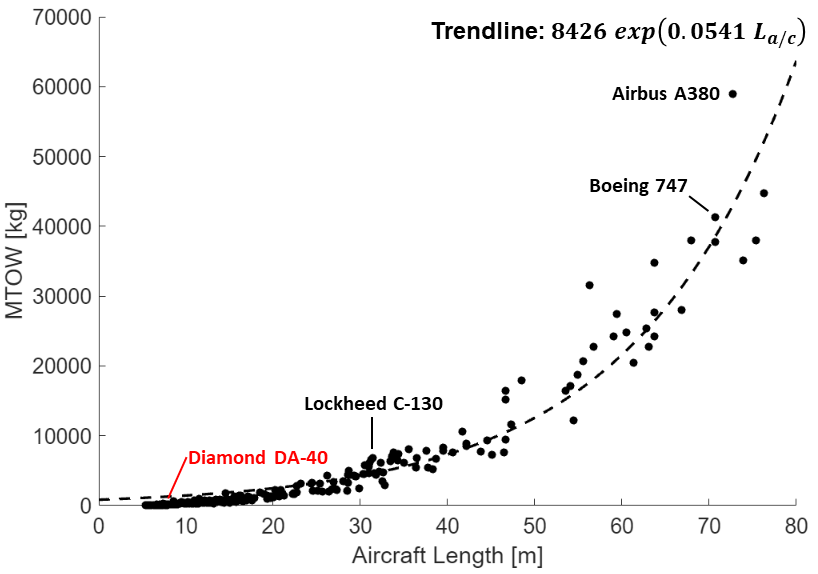
\includegraphics[width=.6\linewidth]{Figures/weights.png}
    \caption{Aircraft with a larger Max Takeoff Operating Weight (MTOW) typically have more space for more complex sensor suites compared to their General Aviation counterparts~\cite{AircraftCharacteristicsDatabase}.}
\end{figure}

Smaller aircraft are not allowed these luxuries, being manufactured with fewer sensors, overall making them less safe. Table~\ref{tbl:sensorsuitecomparison} compares the different sensors onboard a civilian airliner and a civilian general aviation aircraft.

\begin{table}[!ht]\label{tbl:sensorsuitecomparison}
    \caption{Inexhaustive list of sensors available to commercial and general aviation aircraft. (Adapted from~\cite{DiamondAircraftDA40,customerservicesA380AircraftCharacteristics2020})}
    \centering
    \begin{tabular}{lcc}
        \toprule
        \textbf{Sensor}                    & \textbf{Commercial} & \textbf{General Aviation} \\
        \midrule
        Pitot Tubes                        & \(5\)               & \(2\)                     \\
        Distance Measuring Equipment       & \(2\)               & \(1\)                     \\
        Ultra-High Frequency Sensors       & \(2\)               & \(1\)                     \\
        Very-High Frequency Sensors        & \(3\)               & \(2\)                     \\
        Communication Channels             & \(2\)               & \(2\)                     \\
        Outside Air Temperature Sensors    & \(4\)               & \(1\)                     \\
        Fuel Flow Gauge                    & \(4\)               & \(1\)                     \\
        GPS receivers                      & \(2\)               & \(1\)                     \\
        Inertial Measurement Units         & \(3\)               & \(1\)                     \\
        Satellite Communications           & \(1\)               & {--}                      \\
        Specific Impulse Sensors           & \(6\)               & {--}                      \\
        Weather Radar                      & \(1\)               & {--}                      \\
        Traffic Collision Avoidance System & \(4\)               & {--}                      \\
        Radio Altimeter                    & \(3\)               & {--}                      \\

        \bottomrule
    \end{tabular}
\end{table}

Regardless of size, the sensor suite aboard any flight vehicle is able to provide measurements 50 times greater than that of a GPS receiver, so a sensor fusion algorithm is optimal for this situation. Because sensor measurements have inherit errors due to a variety of factors, they can wander or \textit{dead reckon} through time. GPS measurements, although slower, provide measurements that do not drift at cost of being slightly less accurate. Table~\ref{tbl:sensorfusionframeworks} describes the most common sensor fusion frameworks for GPS and INS platforms.
\begin{table}[!ht]\label{tbl:sensorfusionframeworks}
    \caption{Common sensor fusion frameworks used for GPS and INS collection platforms}
    \centering
    \begin{tabular}{clc}
        \toprule
        \textbf{Name}            & \textbf{Level of Measurement}          & \textbf{Typical Error} \\
        \midrule
        \textit{Loosely-Coupled} & GPS Position and Velocity              & \(1~-~3\) [m]          \\
        \textit{Tightly-Coupled} & GPS Pseudorange and Doppler            & \(1~-~2\) [m]          \\
        \textit{Deeply-Coupled}  & GPS Inphase and Quadrature Correlators & \(\leq0.5\) [m]        \\
        \bottomrule
    \end{tabular}
\end{table}
This work presents a deeply-coupled sensor fusion algorithm known as vector tracking. Of the 3 types of GPS and INS sensor fusion frameworks, it is well-documented that deeply coupled provides the most accurate localization between measurement updates~\cite{wattsGPSGLONASSL12019}.
\section{Prior Art}
The objective of this thesis is to investigate the efficacy of position estimation for a flight vehicle in GPS-degraded and GPS-denied conditions. This thesis will analyze the performance through use of a deeply-coupled sensor fusion algorithm utilizing both INS and GPS measurements. The idea of fusing INS measurements and GPS measurements together on a flight vehicle is well-documented. The following subsections scratch the surface of work performed by other authors and their contributions to the field.
\subsection{Sensor Fusion Overview and Variation}
Sensor fusion between GPS and other sensors aboard flight vehicles has existed for years and continues to be developed. A precise, accurate, and robust navigation solution is achievable when redundant, expensive, and high-quality sensor are installed. More information about the sensors found aboard commercial aircraft and smaller aircraft can be found in~\cite{airbuscustomerservicesAirbusA380Aircraft2020} and~\cite{DiamondAircraftDA40}, respectively. Salmon~\cite{salmonExperimentalExplorationLowCost2015} provides an exploratory analysis using ground vehicles and their sensors complimented with a Ground Vehicle Dynamic Model (GVDM) in a tightly-coupled GPS/INS/GVDM sensor fusion. The work of Rhudy~\cite{rhudyDynamicModelaidedSensor2017} is similar to the research presented in this thesis as they present use of known controller inputs into a propriety nonlinear flight vehicle model to perform GPS sensor fusion with low-cost IMUs. Martin~\cite{martinGPSCarrierPhase2017} develops an improved carrier phase tracking approach for precise positioning and vehicle attitude estimation. The vector tracking algorithms described by Martin will be adapted for the GPS and flight vehicle simulation utilized in this thesis.

\subsection{Vehicle Dynamic Model Sensor Fusion}
One of the more common ways to simulate and model a flight vehicle is to use known aerodynamic coefficient tied in with classical flight dynamics to propagate the states in time. The NAVION aircraft model is a nonlinear mathematical aircraft model that uses known aerodynamic coefficient from a single propeller fixed wing Navion aircraft~\cite{nelsonFlightStabilityAutomatic1998}. Rhudy~\cite{rhudyDynamicModelaidedSensor2017} uses the NAVION model included in a Loosely-Coupled sensor fusion with IMU and GPS\@. The paper focuses on using a known aircraft model with incoming piloted control inputs to predict the attitude of the aircraft in time. Khaghani and Skaloud simulate a UAV using initially, known aerodynamic coefficients but feature the coefficients in their Loosely-Coupled sensor fusion algorithm to continuously estimate these variables in their vehicle model. This allows the vehicle dynamic model to change during time as the simulated UAV loses weight due to fuel.Both paper fuse the dynamic model with GPS and IMU measurements at position and velocity level (Loosely-Coupled).~\cite{rhudyDynamicModelaidedSensor2017} uses an Unscented Kalman Filter (UKF) in the navigation filter for \textit{ease of implementation} while Khaghani~\cite{khaghaniAutonomousVehicleDynamic2016,khaghaniAssessmentVDMbasedAutonomous2018} uses a Extended Kalman Filter (EKF) because the 47 state estimation is cumbersome and computationally intensive for the UKF\@. Both Rhudy and Khaghani use simulation environments to perform a monte-carlo analysis. Each IMU is modeled with bias and integrated white noise as a first-order Gauss-Markov process with numbers that mirror IMU of MEMs quality. Because of the simplified vehicle model in~\cite{rhudyDynamicModelaidedSensor2017}, the GPS measurements are not modeled with any noise. However,~\cite{khaghaniAutonomousVehicleDynamic2016} models GPS measurements as white noise with a variance of 1 meter in the North, East, and Down directions. Three years later Khaghani and Skaloud improve the original filter implementation by adding a barometer sensor to the measurement update along with the already standing IMU and GPS measurements. Along with the analysis of the improved filter in simulation, the authors also performed an experimental scenario, building a fixed-wing, single propeller UAV similar to the aircraft simulated in this thesis.

\subsection{Other Types of Flight Vehicle Sensor Fusion}
Other research to localize flight vehicles in GPS-denied environment revolves around fusing together multiple sensors including Ultra Wide Band (UWB) radios, LiDAR and vision-based algorithms. Dong~\cite{dongIntegratedUWBIMUVisionFramework2022} integrates IMU, UWB, and computer vision for the autonomous approach and landing of a small UAV onto a moving platform. The vision framework operates on identifying and tracking independent ArUco markers to calculate the size of the landing zone. The IMU and UWBs work in tandem in estimating the states of the UAV and distance to the landing platform. The UWB radio provide updates at a high frequency but suffer from noise and dropouts when the UAV is farther away from the landing platform~\cite{dongIntegratedUWBIMUVisionFramework2022}. Gr\'of~\cite{grofPositioningAircraftRelative2022} develops a similar algorithm for detecting a runway using a down-view monocular camera, barometer readings, IMU, and previously recorded air data. Mostly because of the camera, both of the aforementioned papers provide bounded results for position and attitude estimation. Also because of the camera, the system is more complex and expensive, 2 things avoided in this work.

\section{Field Contributions}
The focus of the research presented in this thesis is the performance evaluation of localization in GPS-degraded and GPS denied environments for simulated low-cost sensors aboard a small general aviation fixed wing flight vehicle. Taking that into consideration, the following contributions to the field are made:
\begin{itemize}
    \item Determination of the optimal flight vehicle model to use in the navigation algorithm when considering complexity and computational performance.
    \item Comparative analysis of multiple flight scenarios reflecting realistic flight plans and GPS degradation.
    \item Analysis of deeply-coupled sensor fusion algorithm using the flight vehicle model and simulated GPS measurements to determine the efficacy of safe localization in a real-life scenario.
\end{itemize}

\section{Thesis Outline}
The rest of this work follows a description of the physical systems simulated and modeled in the FVDM, satellited simulator, and GPS receiver. After, a presentation of the results, coupled with a Monte-Carlo analysis as a performance evaluation are shown. Wrapping up, final conclusion about the investigation are made and future work considerations are presented.
\chapter{\textbf{Flight Vehicle Dynamics Model}}
The aircraft modeled in this thesis is the Diamond DA-40 single propeller fixed wing aircraft (Figure~\ref{fig:DA40}). The simulation is a full six Degrees of Freedom (DOF) and features 12 control inputs {--} ranging from throttle and control surface inputs to propeller pitch and mixture levers. The sections below detail the flight mechanics modules that propagate the aerodynamics, engine and propeller, landing gear, and gravitational forces and moments during the simulation. Small General Aviation (GA) aircraft are easier to model compared to commercial and military aircraft as performance information for the mechanical components of the plane are not hidden through government or proprietary documents. Using publicly available data, numerical tables can be compiled before simulations to lower the computational burden. The equations of motions and stochastic elements of the model are covered in a later chapter. Heavily important to modeling a flight vehicle, this chapter begins with a discussion of reference frames and how they interact with the proceeding flight mechanics.

\begin{figure}[!ht]\label{fig:DA40}
    \centering
    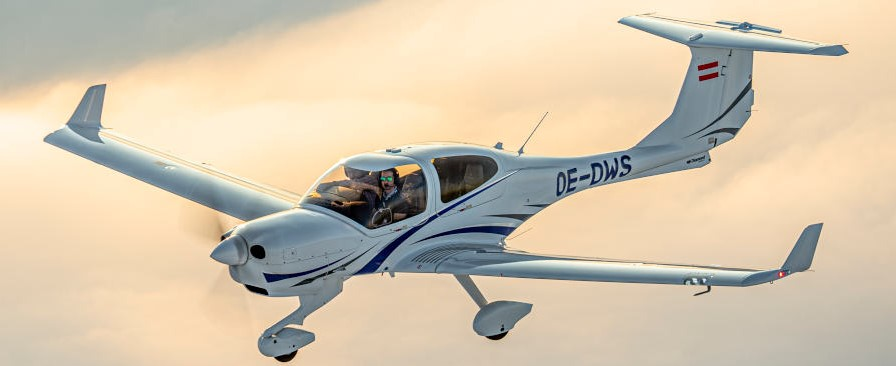
\includegraphics[width=.85\linewidth]{Figures/DA40.jpg}
    \caption{Pilot flying Diamond DA-40 single propeller aircraft~-~the focus of the collection platform for this thesis~\cite{DiamondAircraftDA401969}.}
\end{figure}

\section{\textbf{Reference Frames}}
% What are reference frames
Reference frames and their transformations are a critical component to any navigation algorithm. Reference frames describe the orientation of the flight vehicle with respect to a global or local reference point. Because different components of the FVDM are physically located and oriented at unique locations of the Diamond DA-40, multiple reference frames are used to describe the forces and moments these components generate due to their position with respect to the Center of Gravity (CG) of the aircraft. Reference frame transformations are used to transform local forces and moments into a congruent reference frame such that they can be summed together correctly. This section describes the different reference frames used in this work for the development of the flight mechanics modules within the FVDM\@.
% The different reference frames on the aircraft model
% Body
\subsection{\textbf{Flight Vehicle Reference Frame}}\label{section:FVRF}
The flight vehicle reference frame or body frame describes the reference frame with origin at the center of mass of the modeled Diamond DA-40. The body frame maintains alignment shown in Figure~\ref{fig:flightvehiclereferenceframe} and remains fixed to the flight vehicle at all times. The flight vehicle reference frame is essential to the FVDM as all forces and moments are added together in this frame before integration into global and local pose states. In the flight vehicle reference frame, \(x\) always points through the nose of the aircraft, \(y\) points to the right, or \textit{starboard} side of the aircraft, and \(z\) points through the bottom of the aircraft.

\begin{figure}[!ht]
    \centering
    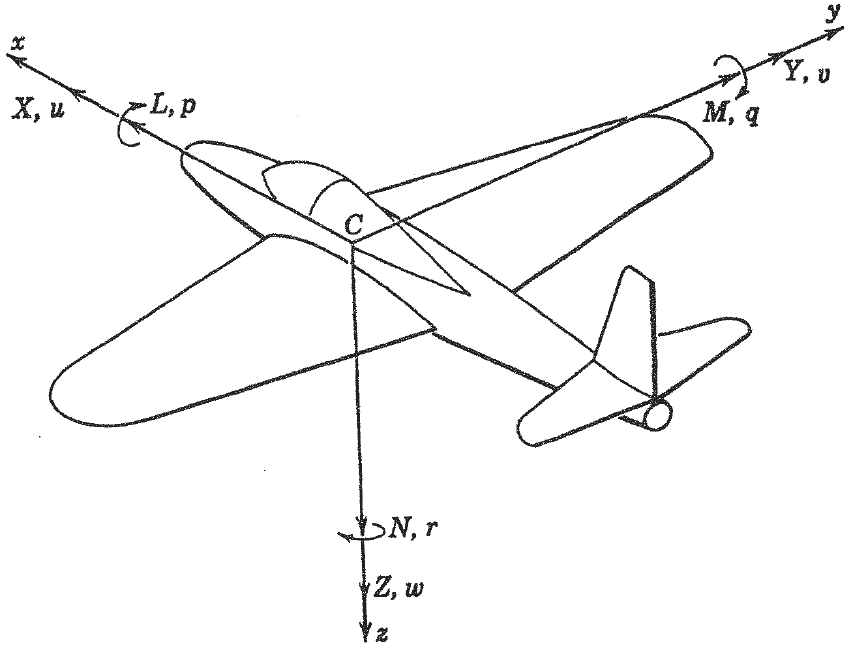
\includegraphics[width=0.60\linewidth]{Figures/bodyframe.png}
    \caption{Standard flight vehicle reference frame used in this work.~\cite{peetSpacecraftAircraftDynamics2021}}\label{fig:flightvehiclereferenceframe}
\end{figure}
\clearpage
% Prop
\subsection{\textbf{Propeller Reference Frame}}
The propeller reference frame describes the axis about which the propeller rotates with origin to the propeller nacelle, as seen in Figure~\ref{fig:propframe}. Propeller \textit{pitch}, as it is referenced in this thesis is a rotation about the \textit{y} axis, while the blades of the propeller rotate about the \textit{x} axis. This axis remains remains fixed in orientation and position.~\( \phi{}\) from Figure~\ref{fig:propframe} describes the twist of the blade. The twist of the blade helps the propeller produce more thrust, but is not used in any reference frame calculations.

\begin{figure}[!ht]
    \centering
    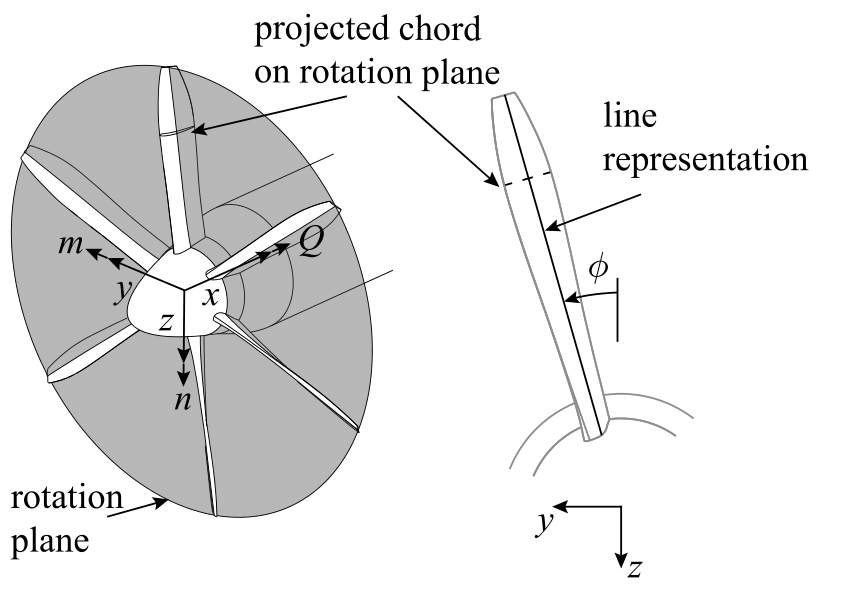
\includegraphics[width=0.75\linewidth]{Figures/propframe.png}
    \caption{The reference frame used to model the dynamic of the propeller in this work~\cite{vanarnhemEngineeringMethodEstimate2020}.}\label{fig:propframe}
\end{figure}

% Wind
\subsection{\textbf{Local Wind Reference Frame}}
The local wind reference frame is used to calculate the lift and drag generated from their respective components with origin at the center of mass of the modeled Diamond DA-40. The orientation of the reference frame changes such that \(\beta \) remains parallel with the trajectory of the aircraft and \(\alpha \) remains parallel to the ground below. In literature, \( \beta \) and \(\alpha \) are referred to as the \textit{sideslip} and \textit{angle of attack} of the aircraft during flight. Sideslip can be thought of as the left or right direction of the aircraft with respect to the incident free stream and angle of attack is the up or down direction of aircraft with respect to the incident freestream.

\begin{figure}[!ht]
    \centering
    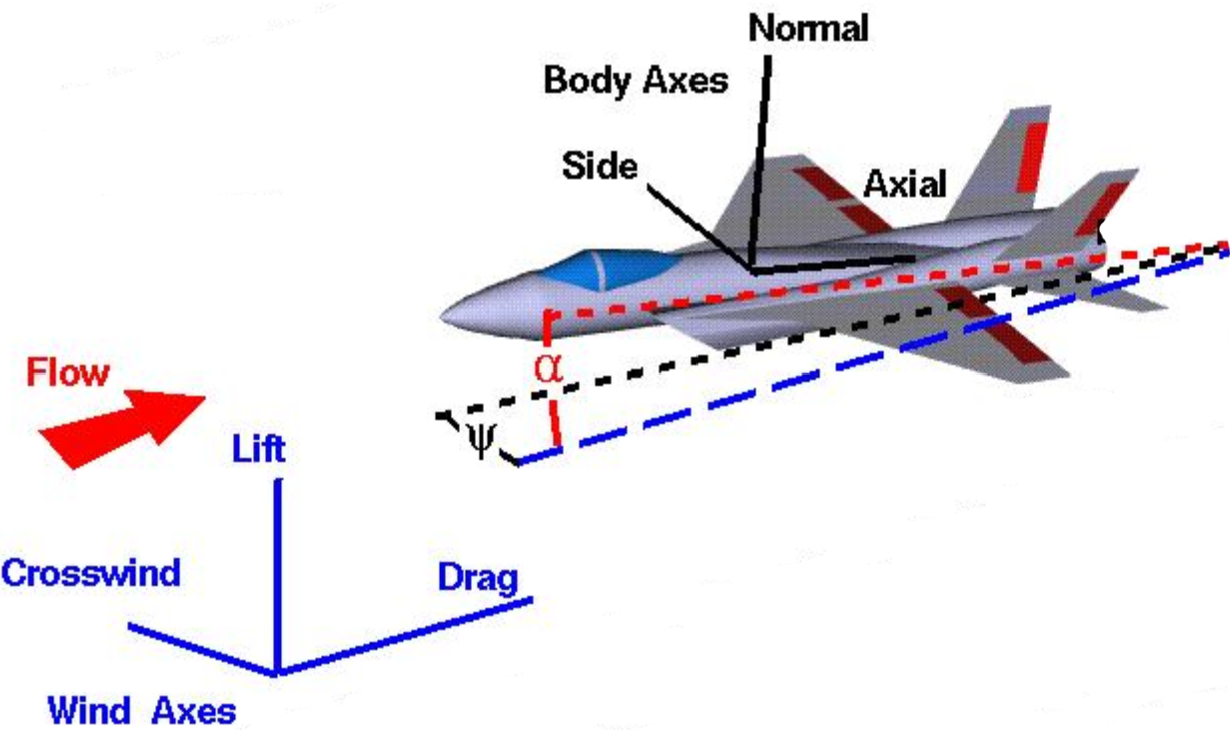
\includegraphics[width=0.75\linewidth]{Figures/windaxes.png}
    \caption{Flight vehicle reference frame and local wind reference frame (dotted lines) (Adapted from~\cite{ForceBalanceCoordinates1969}).}\label{fig:windframe}
\end{figure}

% Local
\subsection{\textbf{Local Navigation Reference Frame}}
A local navigation frame is necessary to define the orientation of the flight vehicle. This work implements a North-East-Down (NED) reference frame in which the axes are aligned with the topographic directions as seen in Figure~\ref{fig:globalframes} by \(X_n\),\(Y_n\), and \(Z_n\). The origin of the local navigation reference frame is defined at the initial position in the FVDM and navigation filter. The Euler attitude angles are used to describe the orientation of the Diamond DA-40 relative to the local navigation frame. When the aircraft has no roll, pitch, or yaw, this equates to the aircraft flying perfectly tangential to Earth's ellipsoid, with the nose of the aircraft pointing towards the North.

\subsection{\textbf{Global Reference Frames}}
Global Reference Frames are critical for GPS receivers to calculate position and velocity. In summary, a position from a receiver is based on distances between the receiver and any visible satellites (details about positioning using GPS satellites is provided in Chapter 3). As all GPS satellites operate in orbit around the Earth, the global reference frame provides a suitable solution that encompasses both satellite and receiver positions and velocities. In this thesis, two global reference frames are used. The Earth-Centered, Earth-Fixed (ECEF) and the geodetic reference system (LLA). The ECEF reference frame is considered the standard global reference frame as it works well for defining both positions and velocities for satellites and receivers, but falls short when it comes to visualization as the origin of the ECEF frame is the center of the Earth. The geodetic reference frame is an alternative frame that allows a visualization advantage by defining positions based on the surface of the Earth. Both LLA and ECEF reference frames utilize the World Geodetic System 1984 (WGS84) to describe Earth's geoid and gravitational field as function of parameters in Table~\ref{tbl:wgs84}. Visualization of both reference frames can be seen in Figure~\ref{fig:globalframes}.

\begin{table}[!ht]
    \caption{Properties describing the WGS84 ellipsoid}\label{tbl:wgs84}
    \centering
    \begin{tabular}{cccc}
        \toprule
        \textbf{Property}          & \textbf{WGS84 Value} & \textbf{Units} \\
        \midrule
        Equatorial Radius, \(R_0\) & 6,378,137.0          & meters         \\
        Polar Radius, \(R_P\)      & 6,356,752.31425      & meters         \\
        Flattening, \(f\)          & 1/298.257223563      &                \\
        Eccentricity, \(e\)        & 0.0818181808425      &                \\
        \bottomrule
    \end{tabular}
\end{table}

\begin{figure}[!ht]
    \centering
    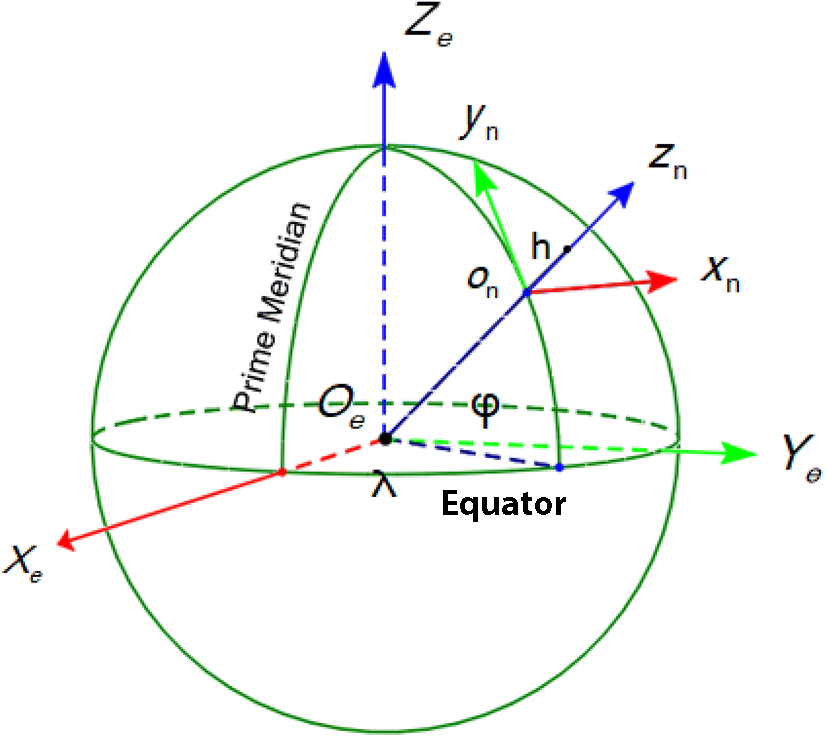
\includegraphics[width=0.75\linewidth]{Figures/globalframe.png}
    \caption{ECEF and geodetic reference frames as used in this thesis.}\label{fig:globalframes}
\end{figure}

% How the reference frames are calculated (DCMs)
\clearpage
\section{\textbf{Reference Frame Transformations}}
Reference frame transformations are critical to any sensor fusion algorithm in order to properly add vectors of different frames together. Reference frame transformations range in complexity, the simplest being a transformation of the NED frame into the East-North-Up reference frame. A more complex transformation could be the global ECEF frame into the body frame. The reference frame transformations used in this thesis are described in the following subsections.

\subsection{\textbf{ECEF to LLA}}

One of the more complicated reference frame transformations is between the two global frames, ECEF and LLA\@. The conversion from LLA to ECEF is provided first in Equations~\ref{eq:meridiancurvature},~\ref{eq:transversecurvature},~\ref{eq:lla2ecefx},~\ref{eq:lla2ecefy}, and~\ref{eq:lla2ecefz}. The variables within these equations are defined in Table~\ref{tbl:wgs84}.

\begin{equation}\label{eq:meridiancurvature}
    R_N (L) = \frac{R_0 \, \left(1 - e^2\right)}{{\left(1 - e^2 \, \sin^2 {\left(L\right)}\right)}^{3/2}}
\end{equation}

Equation~\ref{eq:meridiancurvature}, \(R_N (L)\) describes the one the two radii of curvature. In this case, the meridian radius of curvature describes the north to south radius. The second radii of curvature (Equation~\ref{eq:transversecurvature}) describes the east to west radius and is known as the transverse radius of curvature (\(R_E (L) \)).

\begin{equation}\label{eq:transversecurvature}
    R_E (L) = \frac{R_0}{\sqrt{1 - e^2 \, \sin^2 {\left(L\right)}}}
\end{equation}

After the transverse radius of curvature is calculated, it is used with the LLA positions to calculate the ECEF \(X\), \(Y\), and \(Z\) positions as shown in Equations~\ref{eq:lla2ecefx},~\ref{eq:lla2ecefy}, and~\ref{eq:lla2ecefz}.

\begin{equation}\label{eq:lla2ecefx}
    X_{ECEF} = \left(R_E (L) + h\right)\cos \left(L\right)\cos \left(\lambda\right)
\end{equation}

\begin{equation}\label{eq:lla2ecefy}
    Y_{ECEF} = \left(R_E (L) + h\right)\cos \left(L\right)\sin \left(\lambda\right)
\end{equation}

\begin{equation}\label{eq:lla2ecefz}
    Z_{ECEF} = \left[\left(1 - e^2\right) R_E (L) + h\right] \sin \left(L\right)
\end{equation}

The ECEF to LLA conversion is more complicated. In order to calculate the longitude,\(L\), in Equation~\ref{eq:ecef2llaL}, the altitude, \(h\), (Equation~\ref{eq:ecef2llaaltitude}) must be calculated {--} and vice versa. The correct way to solve for positions in the LLA reference frame is to iterate until the difference between positions from iteration to iteration is miniscule.

\begin{equation}\label{eq:ecef2llaL}
    L = \textrm{atan2}\left(\frac{Z_{ECEF} \left[R_E (L) + h\right]}{\sqrt{X_{ECEF}^2 + Y^2_{ECEF}} \, \left[ \left(1 - e^2\right) R_E (L) + h\right]}\right)
\end{equation}

\begin{equation}\label{eq:ecef2llalambda}
    \lambda = \textrm{atan}\left(\frac{Y_{ECEF}}{X_{ECEF}}\right)
\end{equation}

\begin{equation}\label{eq:ecef2llaaltitude}
    h = \frac{\sqrt{X_{ECEF}^2 + Y^2_{ECEF}}}{\cos\left(L\right)} - R_E (L)
\end{equation}


\subsection{\textbf{LLA to Local}}
The conversion from the LLA reference frame to the local navigation reference frame can be done by forming a Direction Cosine Matrix (DCM),

\begin{equation}\label{eq:ECEF2LNDCM}
    C^{\textrm{n}}_{\textrm{e}} =
    \begin{bmatrix}
        -\sin\left(L\right)\cos\left(\lambda\right) & -\sin\left(L\right)\sin\left(\lambda\right) & \cos\left(L\right)  \\
        -\sin\left(\lambda\right)                   & \cos\left(\lambda\right)                    & 0                   \\
        -\cos\left(L\right)\cos\left(\lambda\right) & -\cos\left(L\right)\sin\left(\lambda\right) & -\sin\left(L\right) \\
    \end{bmatrix},
\end{equation}

and then multiplying the ECEF position vector to produce a position in the NED frame as discussed previously. In Equation~\ref{eq:ECEF2LNDCM}, \(C^{\textrm{n}}_{\textrm{e}}\) describes the DCM used for the transformation. The notation follows such that the subscript (e) is the position in the original reference frame and the superscript (n) is the reference frame the position is being rotated into. This thesis will always follow this notation to avoid any confusion.

\subsection{\textbf{Local to Body}}
Similar to the conversion of LLA to the local navigation frame, the conversion from the local navigation to the flight vehicle reference frame can be done by forming the DCM (Equation~\ref{eq:321DCM}).
\begin{equation}\label{eq:321DCM}
    C^{\textrm{b}}_{\textrm{n}} =
    \begin{bmatrix}
        \textrm{c}_{\theta}\textrm{c}_{\psi}                                                        & \textrm{c}_{\theta}\textrm{s}_{\psi}                                                        & -\textrm{s}_{\theta}                 \\
        -\textrm{c}_{\phi}\textrm{s}_{\psi} + \textrm{s}_{\phi}\textrm{s}_{\theta}\textrm{c}_{\psi} & \textrm{c}_{\phi}\textrm{c}_{\psi} + \textrm{s}_{\phi}\textrm{s}_{\theta}\textrm{s}_{\psi}  & \textrm{s}_{\phi}\textrm{c}_{\theta} \\
        \textrm{s}_{\phi}\textrm{s}_{\psi} + \textrm{c}_{\phi}\textrm{s}_{\theta}\textrm{c}_{\psi}  & -\textrm{s}_{\phi}\textrm{c}_{\psi} + \textrm{c}_{\phi}\textrm{s}_{\theta}\textrm{s}_{\psi} & \textrm{c}_{\phi}\textrm{c}_{\theta} \\
    \end{bmatrix}
\end{equation}
In this case, the DCM comprises of the three Euler angles {--} roll (\( \phi \)), pitch (\( \theta \)), and yaw (\( \psi \)). To allow the matrix to fit the width of the paper, \textit{c} and \textit{s} denote the \textit{cosine} and \textit{sine} trigonometric functions, respectively.

If one wanted to convert position from the body to ECEF reference frame, multiplying Equations~\ref{eq:321DCM} and~\ref{eq:ECEF2LNDCM} provides the user with a DCM to do this (Equation~\ref{eq:ECEF2BODY}).

\begin{equation}\label{eq:ECEF2BODY}
    C^{\textrm{b}}_{\textrm{e}} = C^{\textrm{b}}_{\textrm{n}} \, C^{\textrm{n}}_{\textrm{e}}
\end{equation}

It should be noted that any of these DCM reference frame transformations can be inverted by simply transposing the final transformation matrix.

\section{\textbf{Atmosphere Model}}\label{section:atmos}
In order to more accurately calculate a handful of dynamics modeled in this work, a model of Earth's atmosphere is needed to provide ambient temperature, pressure, and density. This thesis uses the ISA model to approximate ambient temperature, ambient pressure, and ambient density given a certain height above Mean Sea Level (MSL)~\cite{USStandardAtmosphere1976}. Using an assumed linear distribution for temperature as a function of altitude, the ISA model assumes hydrostatic equilibrium as seen by Equation~\ref{eq:2.1},

\begin{equation}
    \frac{dP}{dh} = -\rho \, g,
    \label{eq:2.1}
\end{equation}

where \(\frac{dP}{dh}\) is the vertical pressure gradient as a function of air density, \( \rho \), and acceleration due to gravity, \(g\). After integrating Equation~\ref{eq:2.1}, the ISA model uses the ideal gas law (Equation~\ref{eq:2.2})

\begin{equation}
    P = \rho \, R\textsubscript{air} \, T
    \label{eq:2.2}
\end{equation}

to solve for the ambient pressure \(P\), and density, \( \rho \). A complete form of the ISA model is seen in Equations~\ref{eq:2.3} and~\ref{eq:2.4}.

\begin{equation}
    P = P_0\,\exp\left({\frac{-g\,\Delta h}{R\textsubscript{air}\,T}}\right)
    \label{eq:2.3}
\end{equation}

\begin{equation}
    \rho = \rho_0\,\exp\left({\frac{-g\,\Delta h}{R\textsubscript{air}\,T}}\right)
    \label{eq:2.4}
\end{equation}

where \(P_0\) and \(\rho_0\) are atmospheric layer values for pressure and density, respectively; \(R\textsubscript{air}\) is the specific gas constant for air and \(\Delta h\) is difference between the current altitude of the flight vehicle and altitude of the current atmospheric layer. Figure~\ref{fig:atmos} describes these atmospheric parameters from MSL to 85,000 meters above sea level.
\begin{figure}
    \centering
    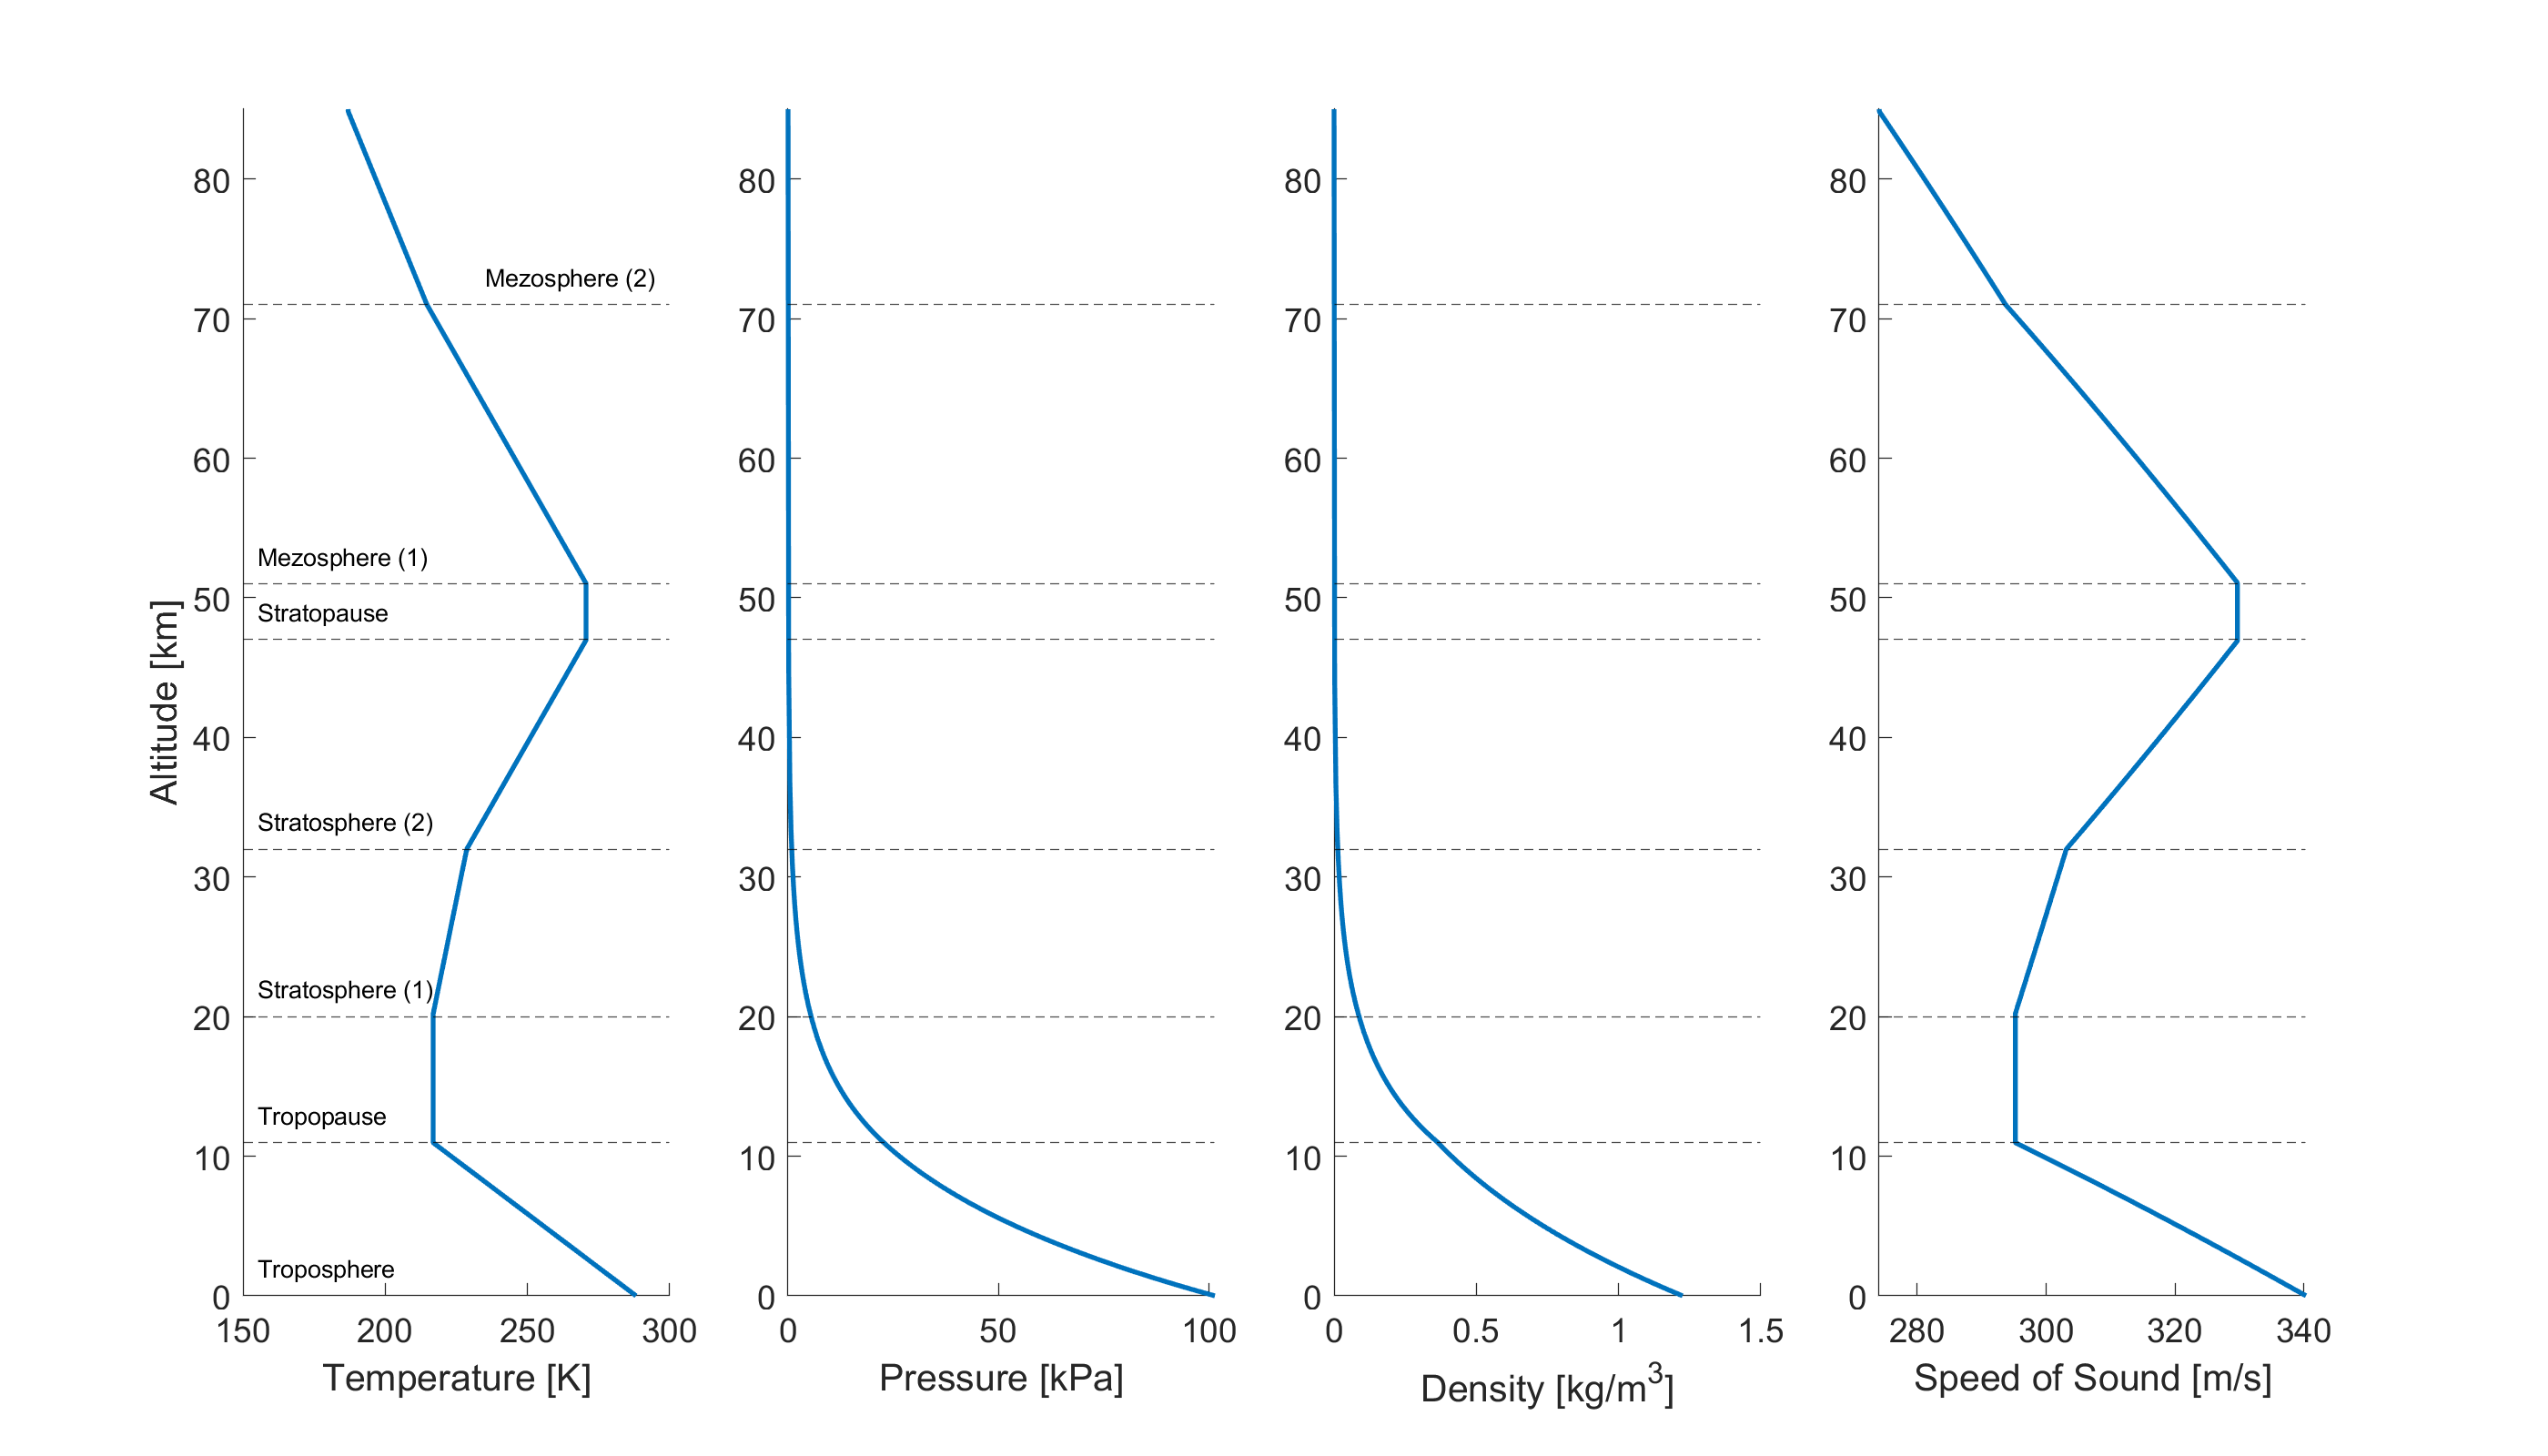
\includegraphics[width=0.8\linewidth]{Figures/atmosphericparameters.png}\label{fig:atmos}
    \caption{Absolute temperature, ambient pressure, air density, and speed of sound using the ISA model.}

\end{figure}

\section{\textbf{Aerodynamic Principles}}\label{section:aerodynamic}
% Section Overview
In all phases of flight, the surfaces on any aircraft generate two aerodynamic forces {--} \textit{lift} and \textit{drag} along with an aerodynamic moment vector. Prior to the modern computer, these forces and moments were derived from swaths of wind tunnel data~(Figure~\ref{fig:windtunnel}) under various conditions. Today, during the research and development phase of modern production aircraft, these aerodynamics components can be determined using Computational Fluid Dynamic (CFD) programs such as \textit{FlightStream}~\cite{FlightStream2022}. This subsection provides the modeling equations for the surfaces of the airplane that generate lift, drag and moments during simulation.

\begin{figure}[!ht]\label{fig:windtunnel}
    \centering
    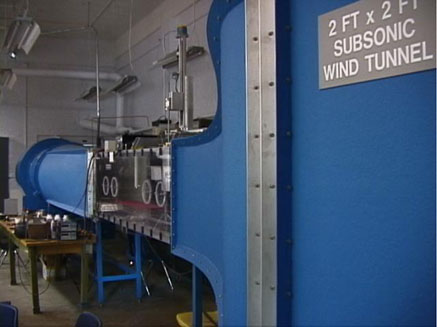
\includegraphics[width=.75\linewidth]{Figures/opencircuitwindtunnel.jpg}
    \caption{Subsonic wind tunnel in Auburn University's Aerodynamics Laboratory.}
\end{figure}

% How is lift generated?

A wing produces lift by allowing the air to move faster over the top of the airfoil. Bernoulli's principle equation (Equation~\ref{eq:bern})

\begin{equation}\label{eq:bern}
    P_1 + \frac{1}{2}\, \rho \, V_1^2 + \rho \, g \, h_1 = P_2 + \frac{1}{2}\, \rho \, V_2^2 + \rho \, g \, h_2
\end{equation}

shows that a faster moving fluid leads to a lower pressure gradient. On the bottom side of the wing, where the air is slower, a higher pressure gradient forms. This difference in pressure creates a force on the wing that lifts the wing and entire airplane into the air (Figure~\ref{fig:pressuregradient})~\cite{WhatLift}.

\begin{figure}[!ht]\label{fig:pressuregradient}
    \centering
    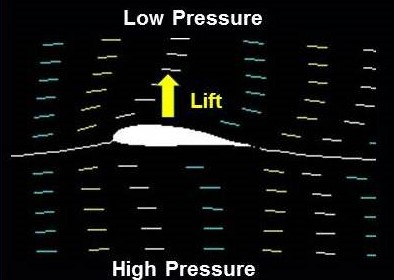
\includegraphics[width=0.75\linewidth]{Figures/foillift.jpg}
    \caption{Pressure gradient and subsequent lift produced onto an airfoil. The continuous white line in the middle signifies the freestream incident wind~\cite{WhatLift}.}
\end{figure}

The lift generated by the wing (and subsequently the aircraft) can be calculated using Equation~\ref{eq:lift}~\cite{raymerAircraftDesignConceptual2018},

\begin{equation}\label{eq:lift}
    L = \frac{C_L \, \rho \, V^2 \, A}{2},
\end{equation}

where \(L\) is the lifting force, \(C_L\) is the lift coefficient for the aircraft, \( \rho \) is the air density, \(V\) is the velocity of the aircraft, and \(A\) is the surface area of aircraft. For the modeling of the Diamond DA-40 presented in this thesis, the aerodynamic coefficients are approximated using {strip theory}~\cite{cookStripTheoryApproach2021}. {Strip theory} is covered in great detail later in this chapter.

% What is drag?
Lift is not the only force produced by the wing during flight. When any object moves through air an opposing force known as drag is generated. For the purpose of the modeling presented in this thesis, drag always opposes the motion of the aircraft. Similar to Equation~\ref{eq:lift}, drag can be calculated using Equation~\ref{eq:drag}.

\begin{equation}\label{eq:drag}
    D = \frac{C_D \rho V^2 A}{2}
\end{equation}

The aerodynamic moments generated during flight of any aircraft are the single reason that control surface deflections cause the aircraft the roll, pitch or yaw in a certain direction. Just like the equations for lift and drag, the total aerodynamic moments are described by equations~\ref{eq:Lmoment},~\ref{eq:Mmoment}, and~\ref{eq:Nmoment}.

\begin{equation}\label{eq:Lmoment}
    M_l = \frac{C_l \rho V^2 A}{2}
\end{equation}
\begin{equation}\label{eq:Mmoment}
    M_m = \frac{C_m \rho V^2 A}{2}
\end{equation}
\begin{equation}\label{eq:Nmoment}
    M_n = \frac{C_n \rho V^2 A}{2}
\end{equation}

% What is Strip Theory?
In Equations~\ref{eq:lift},~\ref{eq:drag},~\ref{eq:Lmoment},~\ref{eq:Mmoment}, and~\ref{eq:Nmoment}, coefficients need to be defined in order to calculate the aerodynamic forces and moments correctly. If known before hand, these coefficients can be calculated programmatically.~Equation~\ref{eq:CL} describes the equation for finding the lift coefficient.

\begin{equation}\label{eq:CL}
    C_L = C_{L_0} + C_{L_\alpha}\alpha + C_{L_q}\frac{qc}{2V} + C_{L_{\delta_e}}\delta_e
\end{equation}

Where \(C_{L_0}\) is the zero angle of attack lift coefficient, \(C_{L_\alpha}\) is the lift coefficient due to angle of attack, \(\alpha \) is the angle of attack,\(C_{L_q}\) is the lift coefficient due to the dynamic pressure, \(q\), and \(C_{L_{\delta_e}}\) is the lift coefficient due to the elevator deflection, \(\delta_e\).~\(c\) is the chord length of the wing and \(V\) is the velocity of the aircraft. Equation~\ref{eq:CD} describes the equation for finding the drag coefficient.

\begin{equation}\label{eq:CD}
    C_D = C_{D_0} + K\,C_{L}^2
\end{equation}

Where \(C_{D_0}\) is the zero angle of attack drag coefficient and \(K\) is the lift induced drag coefficient of the aircraft.

The aerodynamic moment coefficient is split into three components, each defined by the direction they act about the flight vehicle (described by Section~\ref{section:FVRF}). The rolling, pitching, and yawing moment coefficients are described by their respective Equations~\ref{eq:rollingmomentcoefficient},~\ref{eq:pitchingmomentcoefficient}, and~\ref{eq:yawingmomentcoefficient}.

\begin{equation}\label{eq:rollingmomentcoefficient}
    C_l = C_{l_\alpha}\alpha + C_{l_\beta}\beta + \frac{b}{2V}\left(C_{l_p}p + C_{l_r}r\right) + C_{l_{\delta_e}}\delta_e + C_{l_{\delta_a}}\delta_a + C_{l_{\delta_r}}\delta_r,
\end{equation}
\begin{equation}\label{eq:pitchingmomentcoefficient}
    C_m = C_{m_0} + C_{m_\alpha}\alpha + C_{m_\beta}\beta + \frac{c}{2V}\left(C_{m_{\dot{\alpha}}}\dot{\alpha} + C_{m_q}q\right) + C_{m_{\delta_e}}\delta_e
\end{equation}
\begin{equation}\label{eq:yawingmomentcoefficient}
    C_n = C_{n_\alpha}\alpha + C_{n_\beta}\beta + \frac{b}{2V}\left(C_{n_{p}}p + C_{n_r}r\right) + C_{n_{\delta_e}}\delta_e + C_{n_{\delta_a}}\delta_a + C_{n_{\delta_r}}\delta_r
\end{equation}

In the above equations, \(C_{{(.)}_{(.)}}\) are the coefficients relating to their respective aircraft states.~\(p\), \(q\), and \(r\) are the angular rates about the forward, right, and down direction in the flight vehicle reference frame.~\(\delta_e\), \(\delta_a\), and \(\delta_r\) are control surface deflections of the elevator, ailerons, and rudders, respectively.~\( \beta \) is the sideslip angle of the aircraft and represents the angle between the motion of the aircraft and the direction the aircraft is pointing. Finally, \(b\) describes the half-wing span of the aircraft.

Unless these coefficients and their accompanying variables are somehow known \textit{a priori}, determining what they should be can be cumbersome. However, one way to approximate the coefficients to their true value is to use a CFD program and collect tables of data for the aircraft under various flight condition and control surface deflections. The remaining part of this section describes the process of using \textit{FlightStream} in combination with strip theory to approximate their true values.

For the aircraft presented in this thesis, strip theory is a means to better approximate the lift, drag, and moments coefficients described earlier. Figure~\ref{fig:strips} draws the horizontal and vertical strips the aircraft is discretized into. Their reference frame is static and is defined by the strips position and orientation relative to the center of mass of the aircraft. To rotate the aerodynamic forces generated from each strip, a simple yaw{--}pitch{--}row transformation is used.

\begin{figure}[!ht]\label{fig:strips}
    \centering
    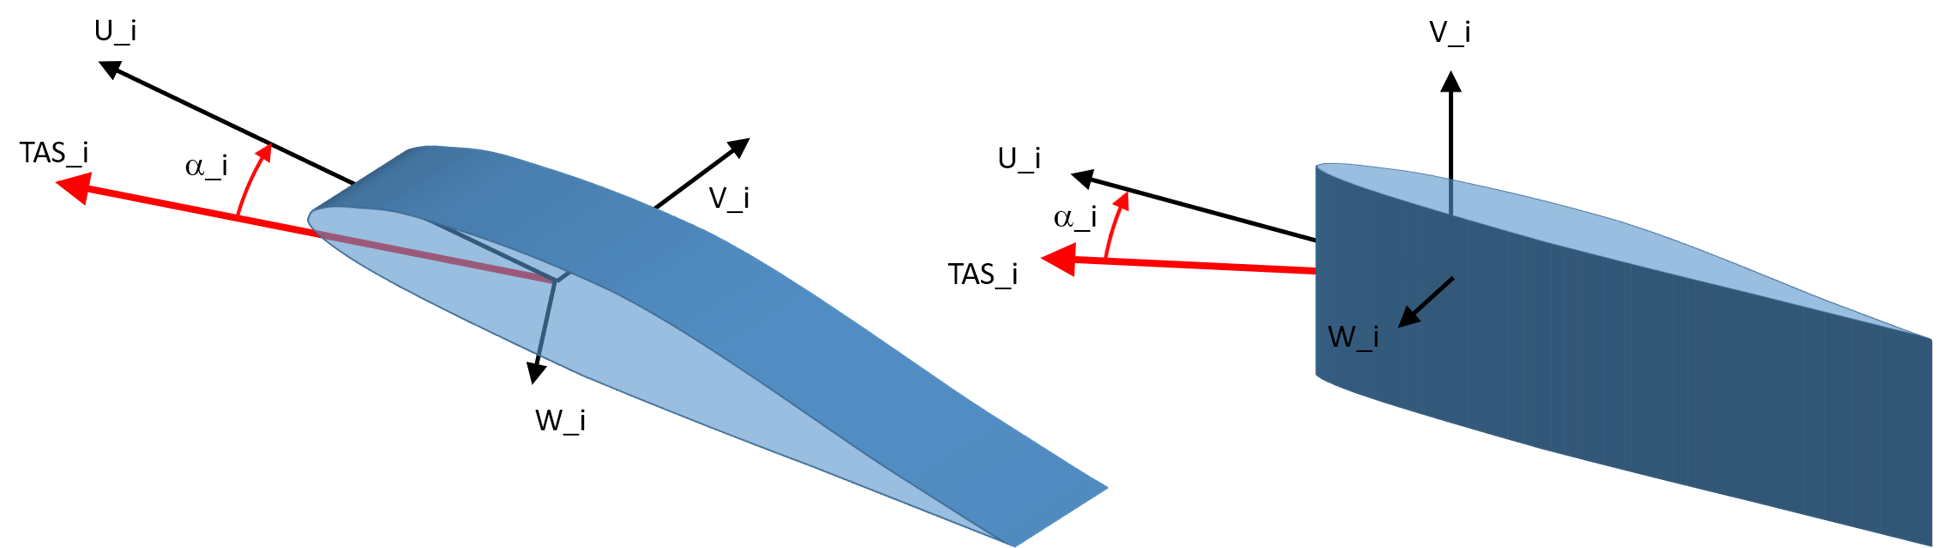
\includegraphics[width=0.75\linewidth]{Figures/horvertstrips.png}
    \caption{Horizontal and vertical strips that are analyzed for aerodynamic coefficients in FlightStream~\cite{AerodynamicStripTheory2021}.}
\end{figure}

Strip theory is a process in which a 3D model of the aircraft is discretized into independent strips and then processed through a CFD program to approximate the performance of the aircraft under various flight conditions. The discretization of the modeled aircraft allows for strip classification where control surfaces are located on the aircraft. Identifying the control surfaces allows the CFD analysis to test different deflection angles, giving a more realistic data set of aerodynamic coefficients when a control surface is actuated (i.e.\ the deflection of the ailerons during a banked turn results in a larger aerodynamic moment compared to flying straight.). FlightStream~\cite{FlightStream2022} is used to generate aerodynamic coefficients for each strip. In FlightStream, the aircraft was evaluated on a range of angles of attack and sideslips, along with different control surface deflections. The aircraft was evaluated at a single velocity of 50 meters per second as the velocity component for the coefficients is just a scaling value.

Downwash is an aerodynamic property where the finite length of the lifting surfaces results in 3-dimensional flow fields causing reduction in effective angles of attack. To introduce downwash into the model and simulation, a reduced-ordered model utilizing integrated circulation was implemented~\cite{ahujaIntegratedComputationalAeroacoustics2022,bhandariGeneticAlgorithmOptimization2023}\@.

\section{\textbf{Aero-Propulsive Forces}}

Calculating lift, drag, and aerodynamic moments are useless unless the aircraft is moving. For any flight vehicle (except a glider), there is some form of engine or propeller that accelerates the incident freestream around the aircraft, allowing the lift, drag, and moment calculations to be of benefit. Similar to a ground vehicle, there is an infinite amount of complexity that can go into the modeling of the propulsive elements within a flight vehicle. The work in this thesis focuses on the engine, shaft, and propeller {--} followed by the effects these components have on the aircraft. The following subsections describe the aero-propulsive flight mechanics that allow aircraft to accelerate, take off, and maintain altitude during the length of the flight.

\subsection{\textbf{Piston Engine Model}}
% Overview of Piston and Propeller Model
Small general aviation aircraft generate propulsive forces through use of an engine that spins a shaft which is connected to a propeller. The engine modeled and simulated is a piston, air-cooled engine. The typical aircraft piston engine is modeled as a four-stroke Otto cycle~\cite{raymerAircraftDesignConceptual2018}. The Otto cycle is a well-known thermodynamic theory that relies on a large air mass flow rate to generate power~\cite{gudmundssonGeneralAviationAircraft2014}. The components of the engine that produce the power are described below.

% Manifold Pressure
Because the engine is air-cooled, one of more important components is the engine manifold. The engine inlet manifold is a set of vents that allow the ambient air to feed directly into the combustion chambers where the oxygen in the air is combusted with the fuel to generate power. Based on the commanded throttle input, these manifold vents can be open or closed to let in more or less air, and in return the engine delivers a proportional amount of power to the shaft. The power production from the engine is heavily reliant on the density of air. The Gagg and Ferrar model,

\begin{equation}\label{eq:gaggandferrar}
    \textrm{power} = \textrm{power}_{0}\left(\frac{\rho}{\rho_0} - \frac{1 - \rho/\rho_0}{7.55}\right),
\end{equation}

relates power production to the density of air. Where \(\rho \) is the density of the ambient air as a function of altitude (Section~\ref{section:atmos}), \(\rho_0\) is the density of ambient air at sea-level on a standard day, and \(\textrm{power}_0\) is the max engine power provided the density ratio and the nominal power production of the engine. From~\cite{hartzellpropellerHartzellPropellerManual2023}, the engine modeled in this work has a nominal power output on a sea-level standard day of 600 horsepower (447.42 kW). Figure~\ref{fig:gaggferrar} shows the power output of the engine modeled in this thesis based on the Gagg and Ferrar model and nominal sea-level power production.

\begin{figure}[!ht]\label{fig:gaggferrar}
    \centering
    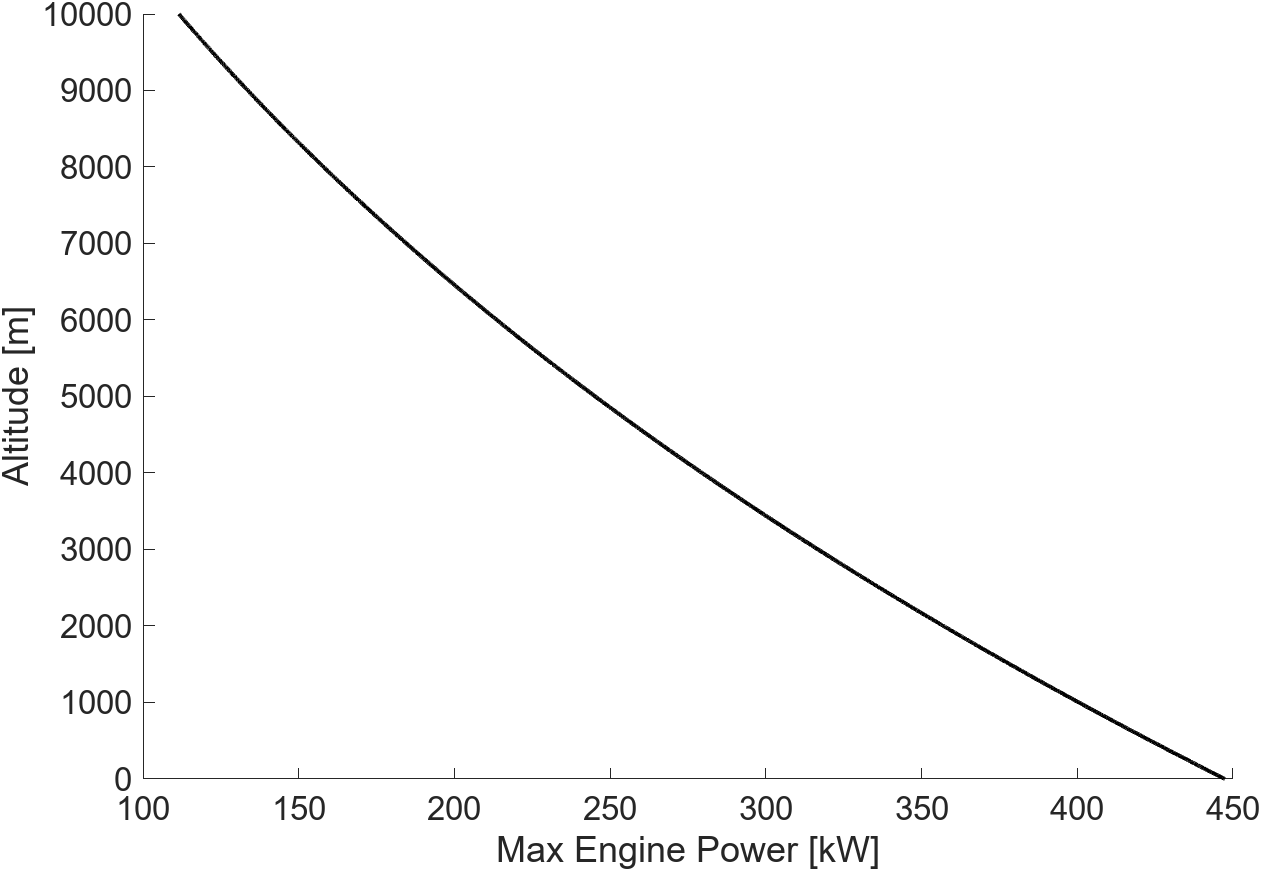
\includegraphics[width=0.85\linewidth]{Figures/gaggferrar.png}
    \caption{Power output for modeled engine as a function of aircraft altitude.}
\end{figure}

However, not all power generated by the engine is absorbed by the shaft. There are losses that include shaft slippage or uneven distribution of fuel inside the combustion chamber. These \textit{errors} are modeled as a power factor and compares the the ideal power produced by the engine to the power absorbed by the shaft. This proportional amount is queried at every time step in the simulation as seen in Figure~\ref{fig:PFLUT}.

\begin{figure}[!ht]\label{fig:PFLUT}
    \centering
    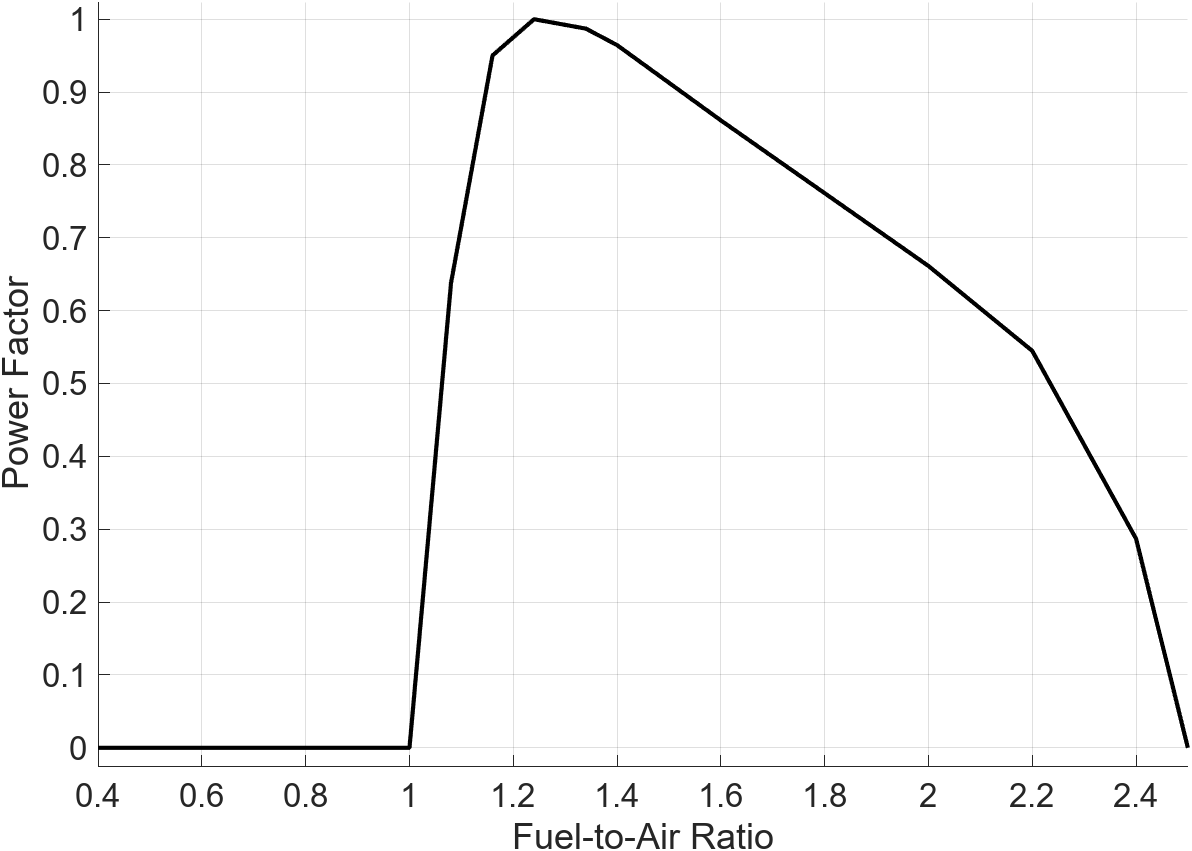
\includegraphics[width=.75\linewidth]{Figures/PFLUT.png}
    \caption{Power factor look up table for modeled engine.}
\end{figure}

% Electric Governor Model
The governor that exists in ground and flight vehicles exists such that drastic changes in throttle do not result in extreme ramps of torque that could structurally damage engine components. It limits the rate of commanded throttle to be linear such that rotational acceleration of the shaft and propeller is safely increased or decreased. The governor also controls fuel consumption of the engine by controlling the engine speed. The fuel consumption is queried at every time step using a look up table that is pre-compiled before the simulation starts (Figure~\ref{fig:BSFCLUT}).

\begin{figure}[!ht]\label{fig:BSFCLUT}
    \centering
    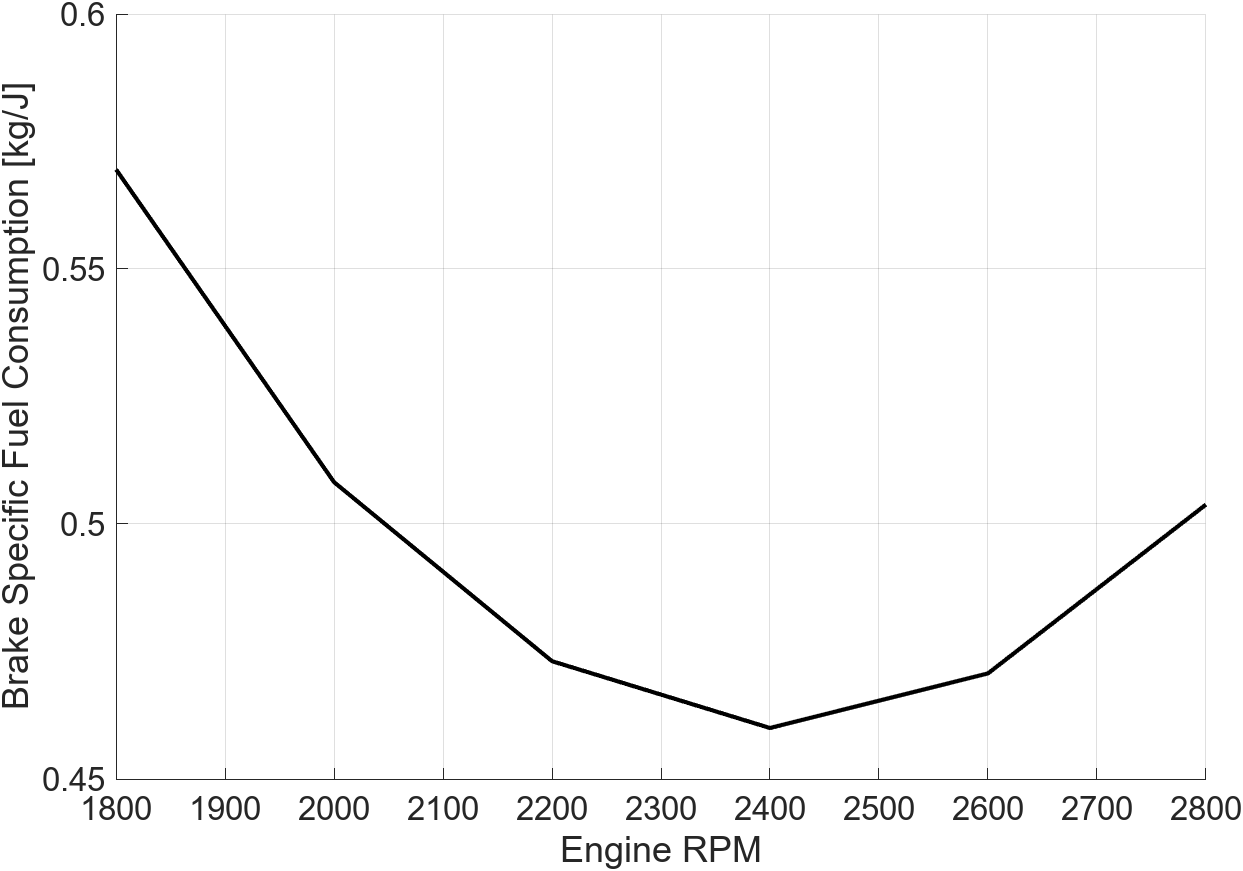
\includegraphics[width=.75\linewidth]{Figures/BSFCLUT.png}
    \caption{Brake specific fuel consumption look up table for modeled engine.}
\end{figure}

\subsection{\textbf{Propeller Modeling}}
% Propeller Dynamics
The purpose of an aircraft propeller is to accelerate the volume of ambient air in front of it such that the lifting surfaces on the aircraft can generate lift and keep the aircraft at altitude. There are 3 main components to focus on when designing and manufacturing propellers. These are the materials used in building the propeller, the number of blades on the propeller, and the curvature and shape of each blade. While the focus of this thesis is not on details in propeller design, it is important to show how the history and differences between these three items affect the efficiency and performance a propeller has in generating thrust power for the aircraft.

The first modern propellers were designed in the early 1900's~\cite{ianHowIdentifyHistoric2016}. Originally made of wood, they featured 3 blades and crudely resembled airfoil shapes (Figure~\ref{fig:woodprops}).

\begin{figure}[!ht]\label{fig:woodprops}
    \centering
    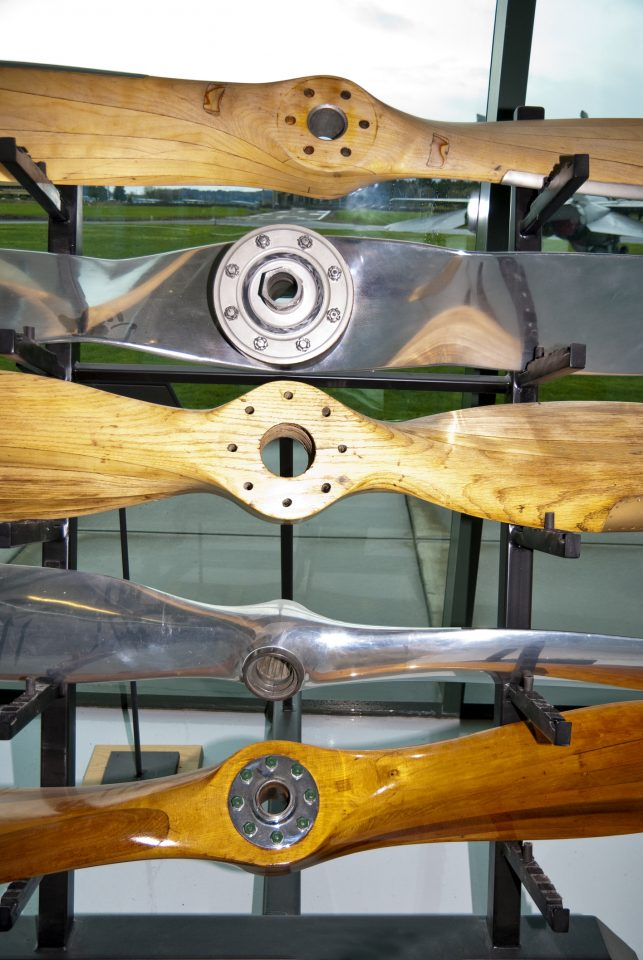
\includegraphics[width=0.3\linewidth]{Figures/woodProps.jpg}
    \caption{Collection of historic wood and steel propellers~\cite{ianHowIdentifyHistoric2016}.}
\end{figure}

These propellers had a fixed pitch, meaning they could not rotate up and down during flight {--} severely costing the propeller thrust power and lowering overall fuel efficiency. In 1929, Wallace Turnbull invented the variable pitch propeller, allowing pilots to control the pitch of the propeller, dramatically increasing propeller efficiency during flight~\cite{ianShortHistoryAircraft2018}. Through time and the advent of computers, CFD analyses shaped a handful of equations that define the performance and efficiency of propeller design. In this work, a three-blade Hartzell~\cite{HartzellPropellerInc1969} composite propeller is used as it is the Original Equipment Manufacturer (OEM) propeller on the Diamond DA-40 aircraft. This propeller is a variable-pitch, constant speed propeller, meaning the pitch of the propeller is optimally adjusted for the current flight condition, while at the same time, maintaining a constant rotational speed to conserve fuel and hold a consistent propeller efficiency (Equation~\ref{eq:propellerefficiency}).

Before the simulation is started, the propeller is analyzed through \textit{FlightStream}~\cite{FlightStream2022}, a surface vorticity flow solver, to analyze the propeller for its lift coefficient (\(C_L\)) at varying flight conditions (Figure~\ref{fig:flightstreamprop}).

\begin{figure}[!ht]\label{fig:flightstreamprop}
    \centering
    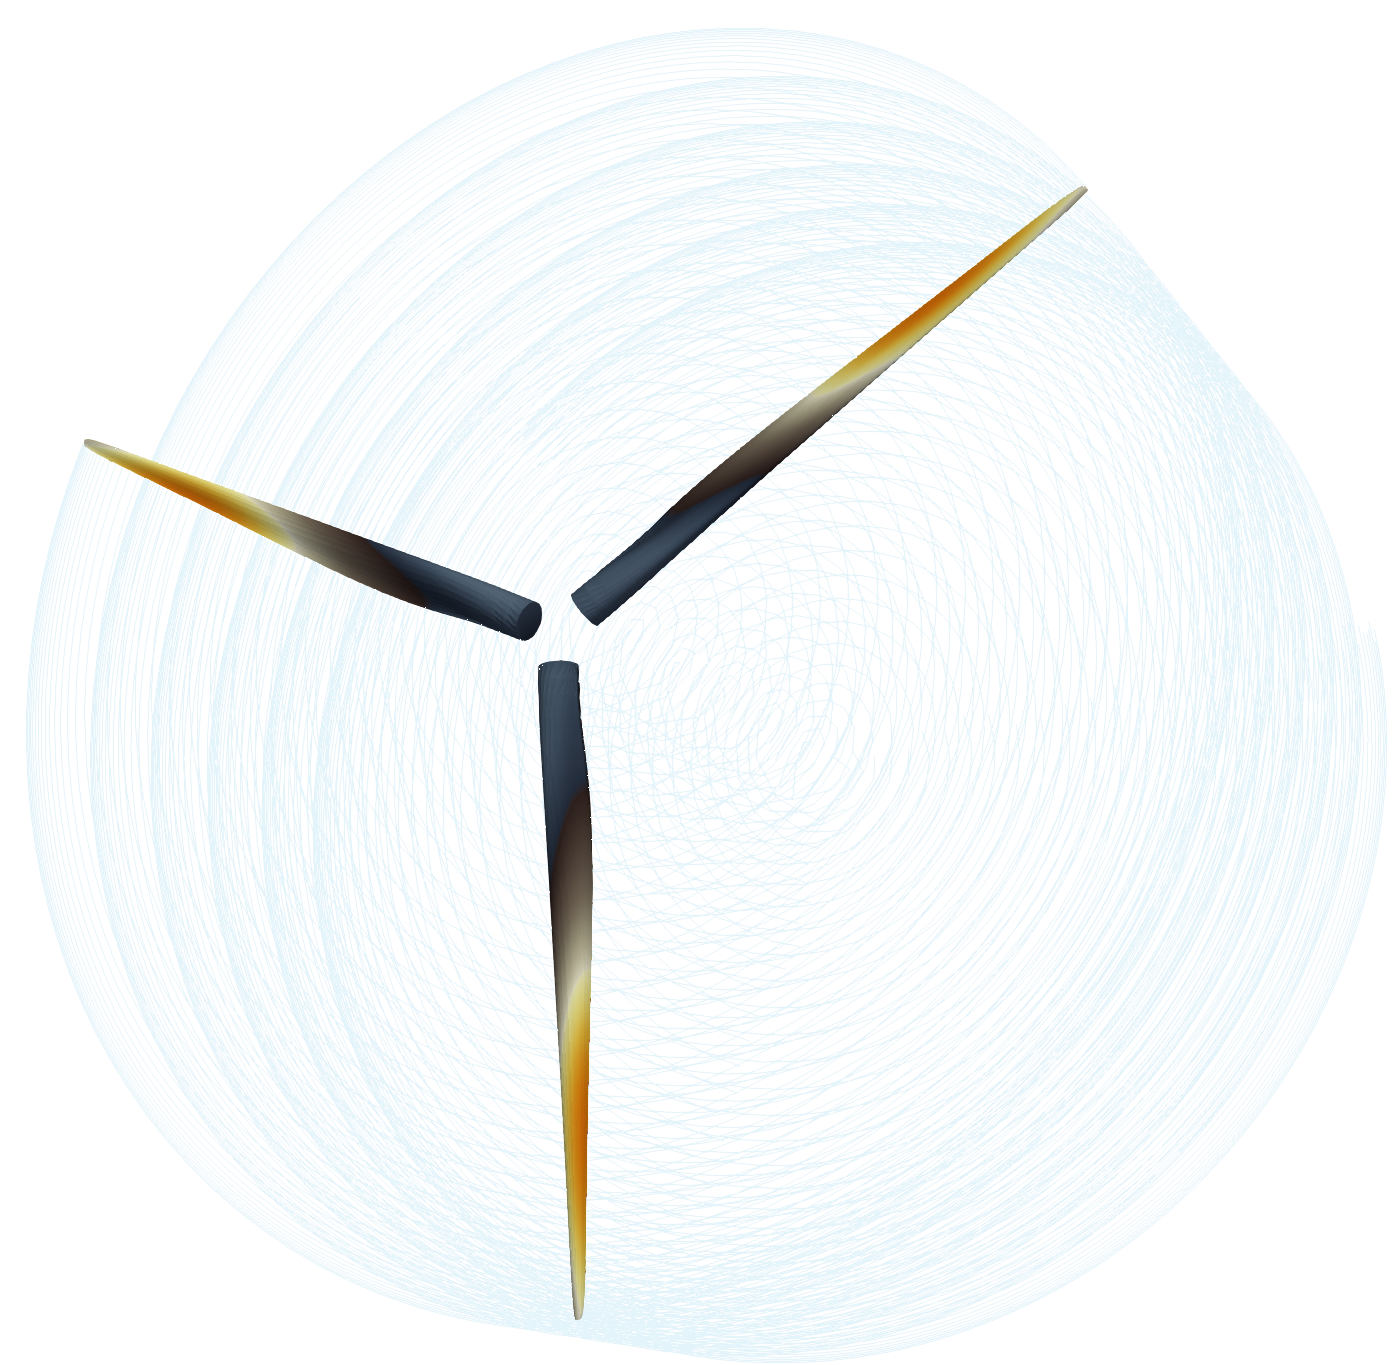
\includegraphics[width=.35\linewidth]{Figures/flightstreamprop.png}
    \caption{Analyzing three-blade propeller through FlightStream~\cite{FlightStream2022}.}
\end{figure}

Once the lift coefficient is determined, numerical look up tables are generated such that the calculation of the forces and moments generated by the propeller can be interpolated, allowing the simulation to be run in real time. To determine the amount of thrust and torque generated by the propeller, the activity factor (Equation~\ref{eq:activityfactor}) of the propeller must first be determined. The activity factor is a measure of the propeller's ability to absorb power and the effectiveness of each blade's width.

% Activity Factor
\begin{equation}\label{eq:activityfactor}
    AF_{\textrm{per blade}} = \frac{1 \times 10^5 \, c_{\textrm{root}}}{16 \, D} \left(0.25 + 0.2 \, \lambda - 0.2 \right)
\end{equation}

Where \(AF_{\textrm{per blade}}\) is the \textit{Activity Factor} per blade, \(c_{\textrm{root}}\) is the length of a blade's chord at the root, \(D\) is the diameter of the propeller, and \( \lambda \) is the taper ratio. Table~\ref{tbl:propparams} describes the design characteristics of the propeller used in this thesis.

\begin{table}[!ht]\label{tbl:propparams}
    \caption{Characteristics of the propeller modeled for this work.}
    \centering
    \begin{tabular}{cccc}
        \toprule
        \textbf{Characteristics } & \textbf{Value} & \textbf{Units} \\
        \midrule
        \(c_{\textrm{root}}\)     & 0.1475         & meters         \\
        \(D\)                     & 1.9            & meters         \\
        \( \lambda \)             & 0.8            & {--}           \\
        \(C_L\)                   & 0.5            & {--}           \\
        \bottomrule
    \end{tabular}
\end{table}

Because the dimensions of the propeller are known, we can determine the activity factor of the blade to be (Equation~\ref{eq:activityfactorcalc},~\ref{eq:activityfactorcalc2})

% Activity Factor Calculation
\begin{equation}\label{eq:activityfactorcalc}
    AF_{\textrm{per blade}} = \frac{1 \times 10^5 \, (0.1475)}{16 \, (1.9)} \left(0.25 + 0.2 \, (0.8) - 0.2 \right)
\end{equation}

\begin{equation}\label{eq:activityfactorcalc2}
    AF_{\textrm{per blade}} = 101.89.
\end{equation}

Now that the \textit{Activity Factor} is known for the modeled propeller, the power (Equation~\ref{eq:powercoefficient}) and thrust (Equation~\ref{eq:thrustcoefficient}) coefficients can be calculated to show how well the propeller generates thrust when the aircraft is static (i.e.\ starting takeoff). For this analysis, we assume the engine to be producing a nominal \(600\) horsepower (\(447.42\) [kW]) and applying a torque equivalent to \(2200\) [rpm] (\(36.6\) [rev\(/\)s]).

% Power Coefficient
\begin{equation}\label{eq:powercoefficient}
    C_P = \frac{P}{\rho \, n^3 \, D^5}
\end{equation}

% Thrust Coefficient
\begin{equation}\label{eq:thrustcoefficient}
    C_T = \frac{T}{\rho \, n^2 \, D^4}
\end{equation}

In Equations~\ref{eq:powercoefficient} and~\ref{eq:thrustcoefficient}, \(P\) is the engine power, denoted in kiloWatts, \(n\) is the rotational speed of the shaft, denoted in revolutions per second, \(T\) is the thrust of the propeller, denoted in kiloNewtons, and \( \rho \) is density of the ambient air. For these calculations, an assumed sea-level density is used (1.225 [\(kg/m^3\)]). Using Figure~\ref{fig:staticpropthrust}, nominal engine power and torque output, we can approximate the thrust coefficient (Equations~\ref{eq:calcCT1},~\ref{eq:calcCT2},~\ref{eq:calcCT3} and~\ref{eq:calcCT4}).

\begin{figure}[!ht]\label{fig:staticpropthrust}
    \centering
    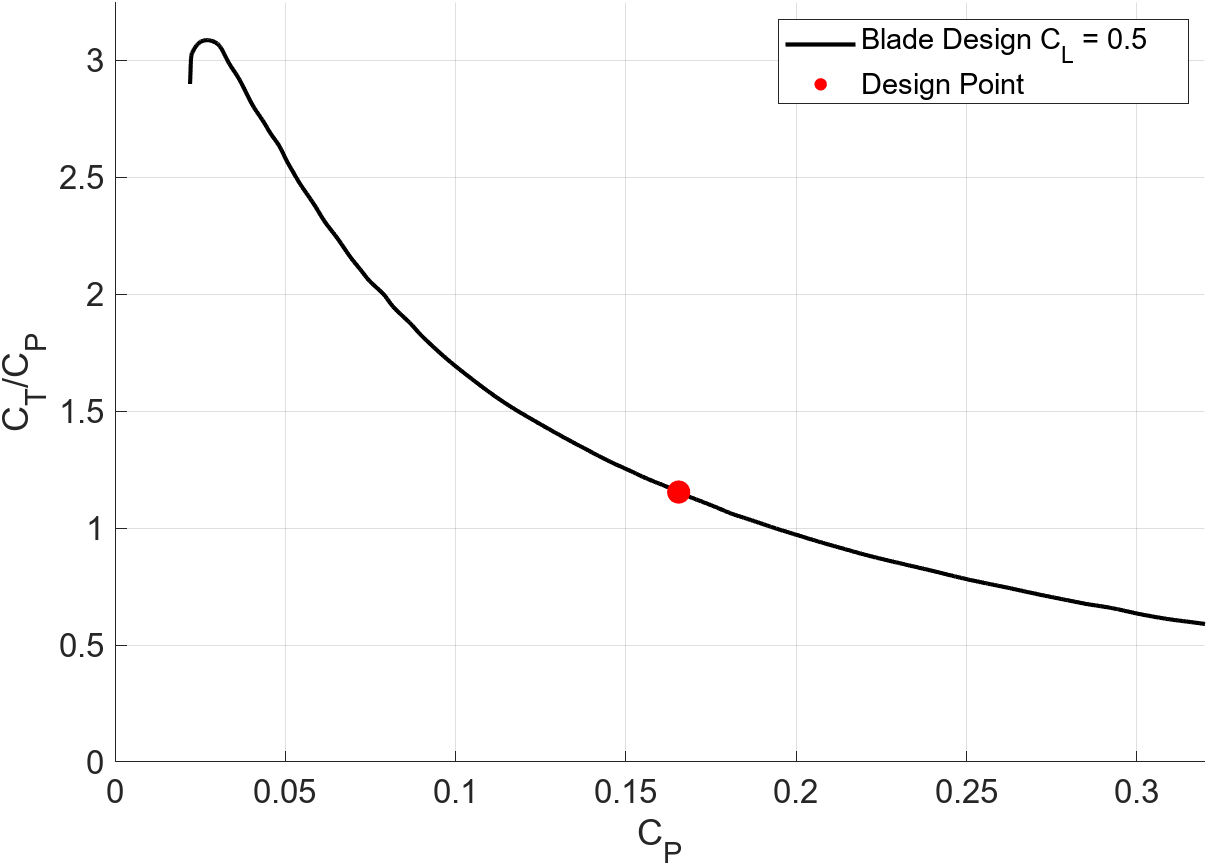
\includegraphics[width=0.85\linewidth]{Figures/StaticThrust.png}
    \caption{Static propeller thrust for the modelled propeller (Adapted from~\cite{GeneralizedMethodPropeller1963}).}
\end{figure}

\begin{equation}\label{eq:calcCT1}
    C_P = \frac{(447.42)(550)}{{(1.225)} \, {(36.6)}^3 \, {(1.9)}^5}
\end{equation}
\begin{equation}\label{eq:calcCT2}
    C_P = 0.16547
\end{equation}
\begin{equation}\label{eq:calcCT3}
    \frac{C_T}{C_P}(@C_P == 0.16547) = 1.1544
\end{equation}
\begin{equation}\label{eq:calcCT4}
    C_T = 0.18997
\end{equation}


Mapping \(C_T\) and \(C_P\) allows for computationally inexpensive queries with calculating propeller efficiency during flight (Equation~\ref{eq:propellerefficiency}).
% Propeller Efficiency
\begin{equation}\label{eq:propellerefficiency}
    \eta_P = \frac{C_T}{C_P} \, J
\end{equation}

Propeller efficiency, \( \eta_P \) compares the amount of power produced by the engine and shaft to the amount of power applied to the ambient air {--} an ideal propeller efficiency would be \(1\), where all of the produced engine power is used to accelerate the ambient air. The \textit{Advance Ratio}, \(J\)
% Advance Ratio
\begin{equation}\label{eq:advanceRatio}
    J = \frac{V}{n \, D} \, ,
\end{equation}

describes how far the flight vehicle moves at each full revolution of the propeller.

The final step in calculating the forces and moments generated by the propeller is querying the thrust based on the previous equations (Equation~\ref{eq:thrust}).
% Thrust
\begin{equation}\label{eq:thrust}
    T = \frac{P \, \eta_P}{V}
\end{equation}

A handful of steps, provided below, list the necessary calculations needed to simulate the thrust for the Diamond DA-40 modeled in this thesis. Because of some of the quantities are constant (i.e.\ propeller diameter and lift coefficient), look up tables can be created before hand to lower the computational load.

\begin{itemize}
    \item[1.] Calculate \(AF_{\textrm{per blade}}\) for given propeller design (Equation~\ref{eq:activityfactor}).
    \item[2.] Query coefficients data table (Figure~\ref{fig:staticpropthrust}) to define \(C_P\) and \(C_T\) (Equations~\ref{eq:powercoefficient} and~\ref{eq:thrustcoefficient}).
    \item[3.] Query \(J\) (Equation~\ref{eq:advanceRatio}) data table for given flight velocity and shaft rotational speed.
    \item[4.] Calculate \( \eta_P \) (Equation~\ref{eq:propellerefficiency}), for given \(J\), \(C_P\), and \(C_T\).
    \item[5.] Calculate \(T\) using Equation~\ref{eq:thrust}.
    \item[6.] The moment generated by the propeller is simply the cross-product between the thrust power and moment arm.
\end{itemize}

\section{\textbf{Landing Gear Model}}
Although not calculated often, the modeling of the aircraft's landing gear are important and should not be overlooked. However, because of the flight paths investigated in this thesis focus solely on the aircraft during flight, a simplified dynamic model is used to describe the forces and moments acting on the landing gear during landing. It should be noted that the aerodynamic calculations of the landing gear occur in the aerodynamically modeling section, while this section focuses on the moments and forces generated from the runway opposing the weight of the aircraft.

To describe the forces and moments generated during landing, a mass-spring damper system (Figure~\ref{fig:ldgfbd}) can be used in simulate the the struts, levers, and tire depression (Figure~\ref{fig:ldg}) that absorb much of the forces, moments and vibrations that act onto the aircraft during landing.

\begin{figure}[!ht]\label{fig:ldgfbd}
    \centering
    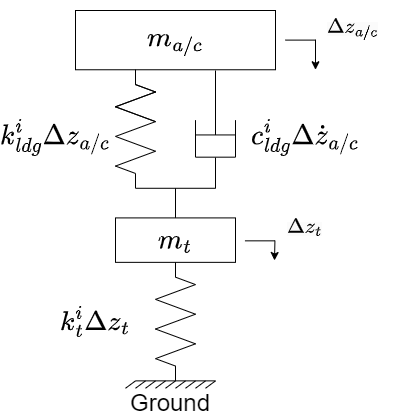
\includegraphics[width=.4\linewidth]{Figures/ldgfbd.drawio.png}
    \caption{Mass-spring damper system, representing the components of landing gear on the aircraft (adapted from~\cite{xingStrengthAnalysisDiagonal2012}).}
\end{figure}

\begin{figure}[!ht]\label{fig:ldg}
    \centering
    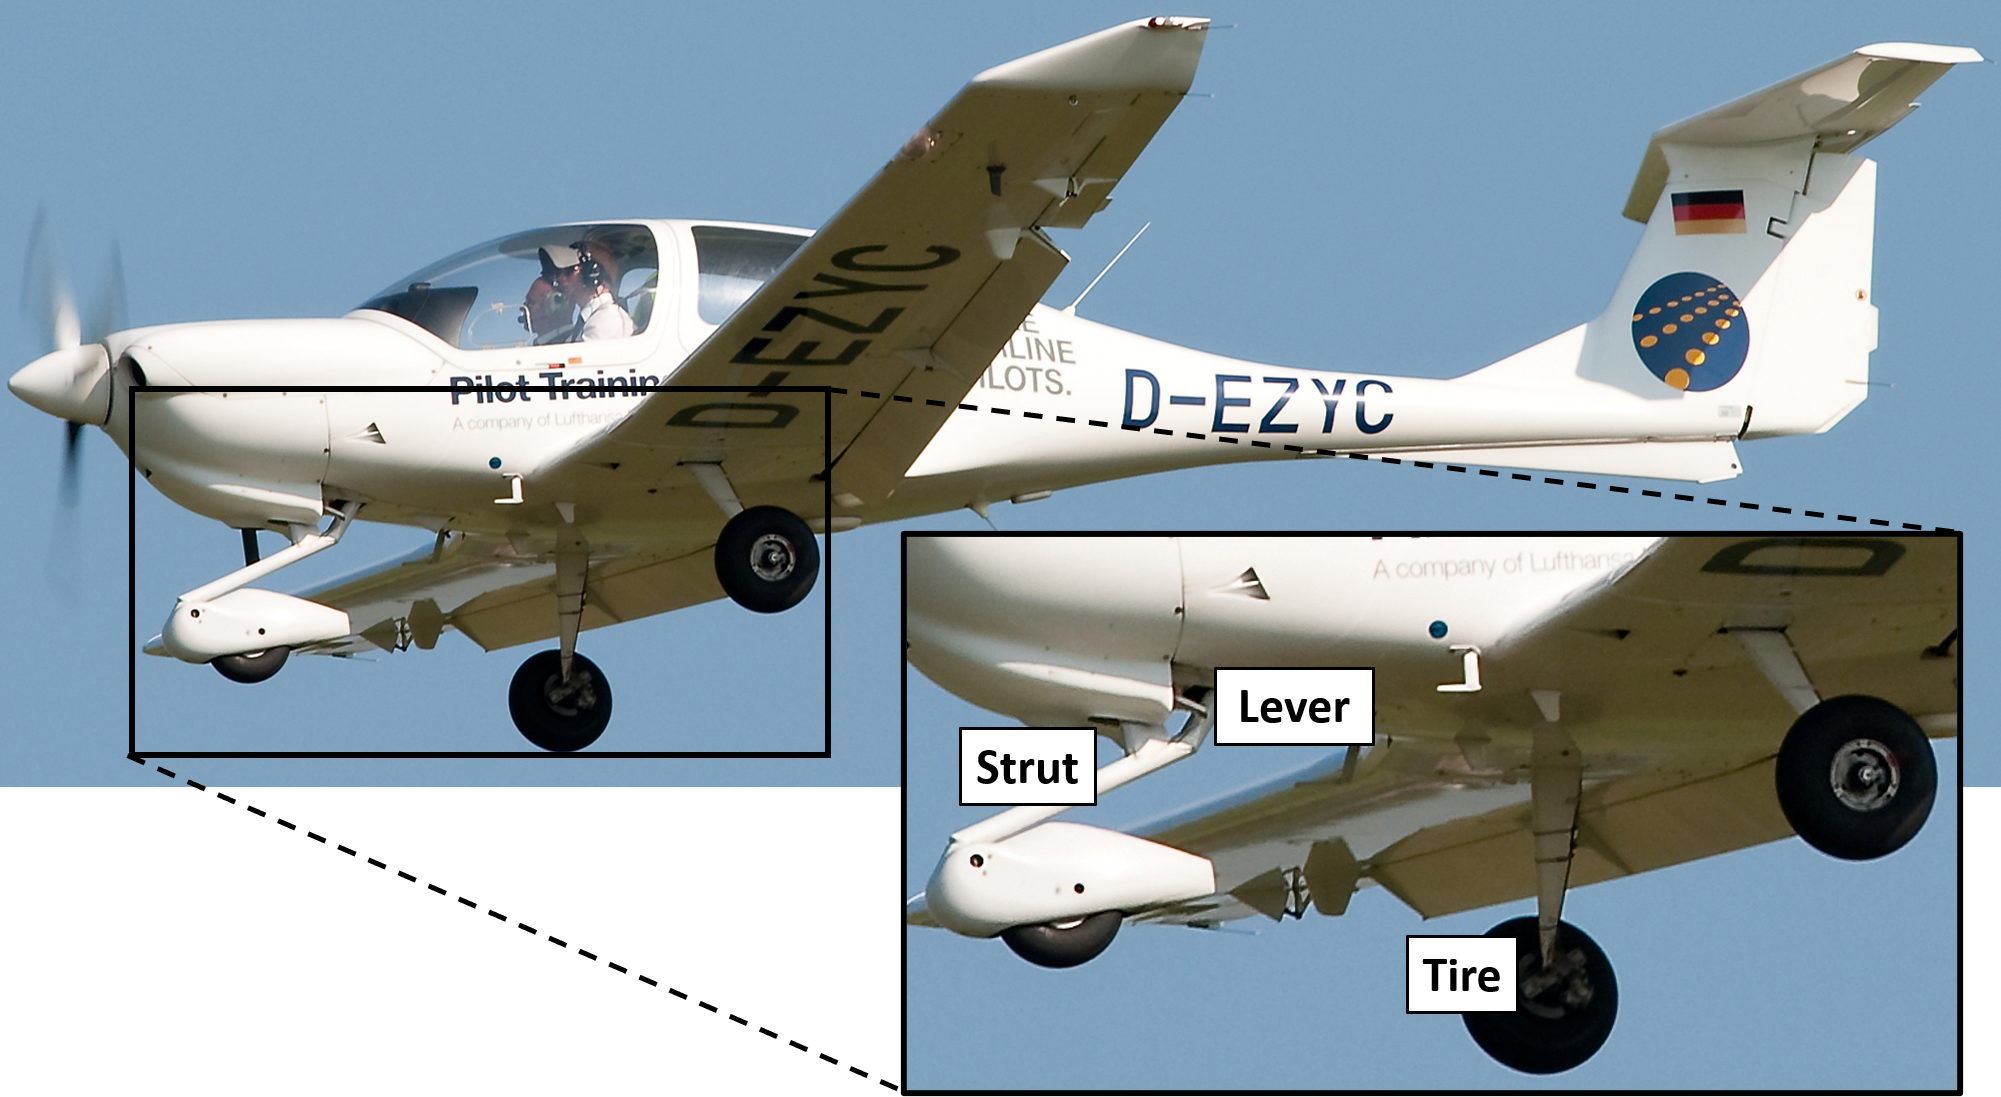
\includegraphics[width=.75\linewidth]{Figures/LandingGear.png}
    \caption{Identification of the landing gear components on the Diamond DA40.}
\end{figure}

Expanding Newton's second law, the forces on each landing gear are solved in the vertical direction (Equation~\ref{eq:ldgforces})

\begin{equation}
    \sum F^i_z = m\,a_z = k^i_t\, \Delta z_t\, + \, k^i_{ldg}\, \Delta z_{a/c}\, + c^i_{ldg}\, \Delta \dot{z}_t,
    \label{eq:ldgforces}
\end{equation}

where \(k^i_{ldg}\) and \(c^i_{ldg}\) are the spring and damper coefficients of the struts and levers respectively (see Table~\ref{tbl:ldgcoeff} for the values used in this simulated model). \(\Delta z_{a/c}\) and \(\Delta \dot{z}_t\), are the deflection and rate of deflection of the aircraft during landing.~\( k^i_t \) and \(\Delta z_t\) are the tire \textit{spring} coefficient and tire depression respectively. For a general aviation aircraft, the depression of the tire upon landing is relatively small such that this term is thrown out.

\begin{table}[!ht]\label{tbl:ldgcoeff}
    \caption{List of spring and damper coefficients for nose and rear landing gear.}
    \centering
    \begin{tabular}{cccc}
        \toprule
        \textbf{i} & \textbf{Location} & \(\mathbf{k}\) \(  \left[\frac{kN}{m}\right]\) & \(\mathbf{c}\) \( \left[\frac{kN\,s}{m}\right]\) \\
        \midrule
        1          & Nose              & \(50\)                                         & \(11.3\)                                         \\
        2          & Rear Right        & \(80\)                                         & \(14.3\)                                         \\
        3          & Rear Left         & \(80\)                                         & \(14.3\)                                         \\
        \bottomrule
    \end{tabular}
\end{table}

The observed moments are solved by taking the cross product between the calculated forces of each landing gear and the moment arm (Equation~\ref{eq:ldgmoments}).

\begin{equation}
    \sum M^i = \textnormal{cross}([\,0\,;\,0\,;\,F^i_z\,],[\,x^i\,;\,y^i\,;\,z^i\,])
    \label{eq:ldgmoments}
\end{equation}

In Equation~\ref{eq:ldgmoments}, \(x^i\), \(y^i\), and \(z^i\) represent the moment arm that is derived from the center of gravity for the aircraft down to where each tire makes contact with the ground.

As a final note, it should be made clear that the forces and moments generated from the landing gear if and only if a tire has made contact with the ground.

\section{\textbf{Forces and Moments Calculations}}
The final product of the aforementioned systems sums to the total force and total moment acting on the body of the aircraft. This work demonstrates the high-fidelity modelling of engines, propellers, landing gear, and aerodynamic forces and moments the simulated flight vehicles generates while in flight. The final step of these calculations is to add them together in the body-fixed \(X\), \(Y\), and \(Z\) directions. This is demonstrated by Equation~\ref{eq:sumForce} and Equation~\ref{eq:sumMoments}.

\begin{equation}
    \sum \mathbf{F} = \mathbf{F}_{prop} + \mathbf{F}_{aero} + \mathbf{F}_{LDG} + \mathbf{F}_{grav}
    \label{eq:sumForce}
\end{equation}

\begin{equation}
    \sum \mathbf{M} = \mathbf{M}_{prop} + \mathbf{M}_{aero} + \mathbf{M}_{LDG} + \mathbf{M}_{grav}
    \label{eq:sumMoments}
\end{equation}

It should be noted that \(\mathbf{F}_{LDG}\) and \(\mathbf{M}_{LDG}\) are only calculated when the aircraft is landing.

Once the forces and moments are calculated, they are used within the equation of motions that propagate the position, velocity, angular rates, and Euler attitude during the simulation of the flight.

\section{\textbf{Measures of Fidelity}}

This focus of this work is the development of a high-fidelity FVDM that closely resembles the behavior of a Diamond DA-40. That being said, the fidelity of the model could always be improved. There is a common question about how much fidelity is needed to provide accurate predictions of the behavior for the modeled flight vehicle. The research performed by~\cite{khaghaniAutonomousVehicleDynamic2016} evaluates this question quite well, where the focus of the work was implementing a 47-state Extended Kalman Filter (EKF) in which 24 of the states were estimating aerodynamic coefficients. For systems where the navigation filter is not fully cognizant of the flight vehicle it is installed on, this method can provide a more generalized solution when extensive knowledge of the flight vehicle does not exist. The work of~\cite{mwenegohaModelbasedTightlyCoupled2020} showcases the value of estimating the aerodynamic coefficients by presenting decent positioning estimates during periods of low satellite visibility.


\section{\textbf{Conclusions}}

This section provided an overview of the reference frames used heavily when calculating the forces and moments the aircraft experiences during flight. Following a discussion of reference frames, the ISA model used in this work was defined with accompanying equations. The bulk of this chapter contains information about the use of strip theory for modeling the aerodynamics of the aircraft and a discussion of the engine and propeller modeling that produces the thrust for the Diamond-DA40 during flight. This chapter concludes with a description of the landing gear model and the summation of the forces and moments generated from the aforementioned sections that will be used in the equations of motions. Because the equations of motions are embedded within the proposed navigation filter for this work, they will be discussed in chapter 4.
\clearpage
\chapter{GPS Software Defined Receiver Architecture}\label{chpater:scalartracking}
Since 1993, the Global Positioning System (GPS) has provided users with capable hardware to determine their global position within seconds and in recent developments, at centimeter-level position error~\cite{bradfordparkinsonGlobalPositioningSystem1996}. The focus of this chapter revolves around the inner-workings of a scalar-tracking software defined receiver, capable of processing GPS L1 C/A. Split into four sections, the chapter begins with an explanation on how the receiver discretizes and digitizes the continuous, low-power signal collected by the antenna. Following that, details about how the receiver knows what satellites are transmitting to it are described. The third section draws on the different algorithms in scalar tracking that allow the received signal data to be replicated and decoded for satellite orbital parameters that play an important role in the last section. Wrapping up this chapter, an overview on the weighted nonlinear least squares algorithm is provided along with detailed descriptions of the three measurements that each satellite is indirectly broadcasting to the receiver.

\section{Front End}
The signals received by an antenna must be down converted and digitized before the processing of the signal can take place. The \textit{Front End} of the receiver performs this conversion through a series of amplifiers, filters, and a Analog-to-Digital Converter (ADC)~\cite{kaplanUnderstandingGPSPrinciples2006}. First, a signal is received by a Right-Hand Circularly Polarized (RHCP) antenna. The antenna can be passive, but for challenging scenarios, a powered, active antenna may be necessary. Because of the low received signal power that GPS constellations provide, the signal is amplified through a series of Low Noise Amplifiers (LNA) and Band Pass Filters (BPF). The LNA raise the power of the received GPS signal and the BPF act as a first-step in removing non-GPS signals from processing. The last stage is passing the continuous received signal through the ADC where the signal is converted to digitized samples at a frequency of the receiver-embedded oscillator. The oscillator is filtered using a phase lock loop (PLL), described later.

The purpose in this mixing process is to transform the signal into a more manageable intermediate frequency while still maintaining the same modulation and Doppler applied to the signal. Figure~\ref{fig:frontend} describes the process on converting the analog, continuous signal into a discrete, digitized IF signal in block diagram form.

\begin{figure}[!ht]\label{fig:frontend}
    \centering
    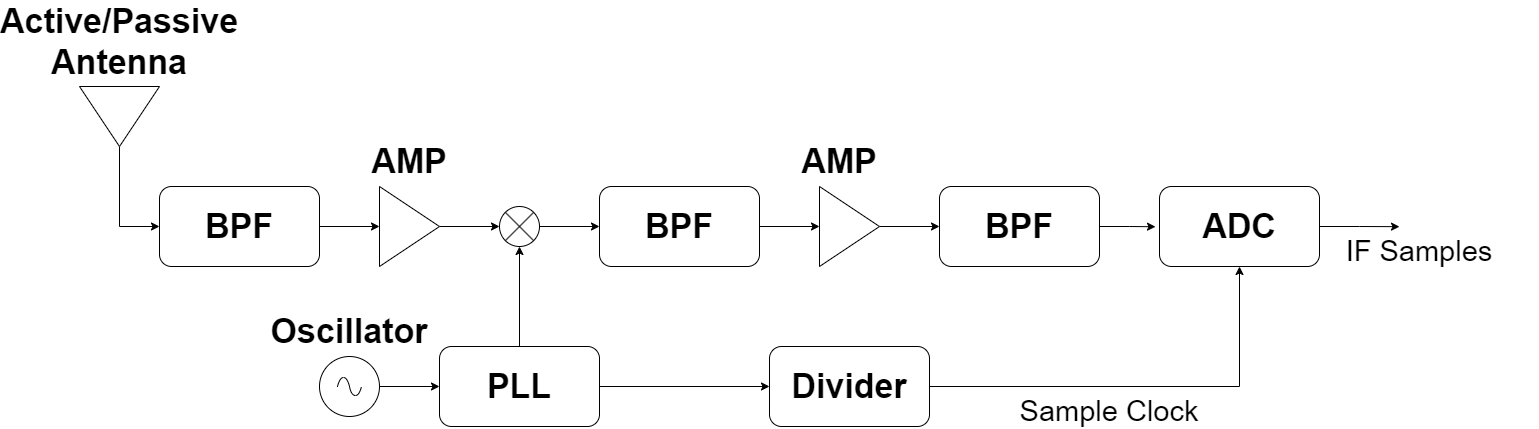
\includegraphics[width=\linewidth]{Figures/frontend.drawio.png}
    \caption{Block diagram of a software defined receiver front end.}
\end{figure}

\section{Acquisition}
Once the received signals are converted to a discrete form, the receiver will determine which satellites are transmitting and in-view. Acquisition correlates local replicas of a signal with the received data. In order for there to be a large correlation magnitude, pseudo-random number (PRN) codes must be within 1-chip and the frequency of the carrier wave must also be within 250 hertz of the true frequency. Correlation with the carrier frequency can be difficult due to the motion of the satellite, and even more difficult if the collection platform is also moving. The motion of the satellites with respect to the receiver bring a change to the carrier frequency known as the Doppler shift. For the algorithms in acquisition to successfully determine which satellites are in-view of the receiver, it is beneficial to correlate with each satellite for the specified constellation, at each code offset, and at a wide range of carrier frequency offsets~\cite{kaplanUnderstandingGPSPrinciples2006}.

A modern, ubiquitous approach to correlating the local replica signals with the received data is using a Parallel Code Phase Search (PCPS) algorithm in which the correlations occur in the frequency domain~\cite{scottRapidSignalAcquisition}. PCPS parallelizes the PRN code offset search space by converting the space from the time to frequency domain. This process is shown in Figure~\ref{fig:PCPS}.

\begin{figure}[!ht]\label{fig:PCPS}
    \centering
    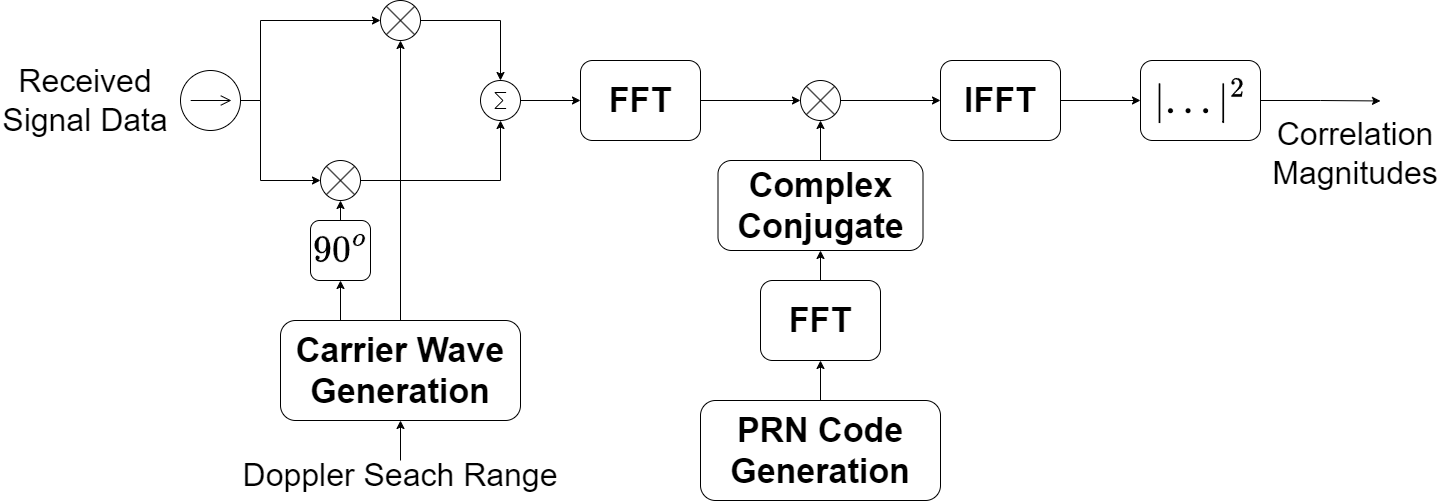
\includegraphics[width=\linewidth]{Figures/PCPS.drawio.png}
    \caption{Block diagram of the PCPS acquisition algorithm applied to GPS L1 C/A signal modulation.}
\end{figure}

To start, the local replicas of the carrier wave are multiplied with the received data across both in-phase and quadrature channels in the complex domain. These resulting multiplications are summed together and passed through a Fast-Fourier Transform (FFT) to convert the vectors into the frequency domain. The second step involves converting the upsampled PRN codes of the satellites to the frequency domain and then applying the complex conjugate to frequency-based, PRN vectors. Multiplying the PRN replicas with the transformed carrier replicas provides the user with a cross-correlation in the frequency domain. To appreciate the correlation magnitudes, the output is passed through an Inverse FFT, converting the correlation values from a frequency domain, complex matrix to a time domain, matrix. The last step requires determining the magnitude of each row in the matrix and then processing the next satellite until all satellites in the constellation are processed. If a correlation exceeds a certain magnitude, its location in the matrix of correlations indicates the estimated PRN code delay and Doppler shift carrier frequency for that particular satellite. The resolution of the PCPS algorithm greatly depends on the grid of Doppler search bins; for a static receiver processing GPS L1 C/A transmissions, a typical resolution is \(-15,000\) to \(15,000\) Hertz in bins of \(500\) Hertz~\cite{scottRapidSignalAcquisition}.

\section{Tracking}
Acquisition provides initial estimates of code delay and carrier frequency for each satellite that is in-view of the receiver. However, because of the motion of the satellites and the receiver (if not static), the delays of the code and changes in the carrier frequencies must continue to be estimated. Tracking performs this process by opening a channel for each in-view satellite. For the duration of the recording, a number of algorithms within tracking continue to correlate the local receiver replica with the received signal data. For scalar tracking, Figure~\ref{fig:scalartracking} describes the flow of how these algorithms produce accurate code replicas for the receiver to calculate satellite PVT solutions.

\begin{figure}[!ht]\label{fig:scalartracking}
    \centering
    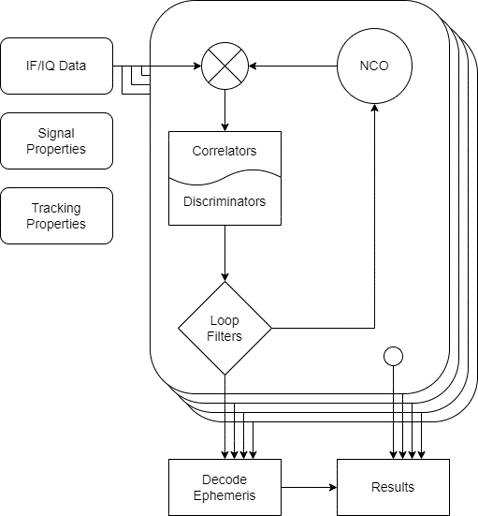
\includegraphics[width=0.5\linewidth]{Figures/scalartracking.png}
    \caption{Flow diagram of scalar tracking algorithms.}
\end{figure}

\subsection{Correlators}
For a receiver to know it is replicating the signal correctly, it generates several correlators that are defined by the error in frequency, phase, and code phase between the replicated signal and the received signal data~(Equation~\ref{eq:correlators}).

\begin{equation}\label{eq:correlators}
    \begin{split}
        IP(k) & = A\,R(\epsilon)\,D(k)\,\cos\left(\pi \,f_{err}\,T + \theta_{err}\right) + \eta_{IP}\\
        QP(k) & = A\,R(\epsilon)\,D(k)\,\cos\left(\pi \,f_{err}\,T + \theta_{err}\right) + \eta_{QP}\\
        IE(k) & = A\,R(\epsilon + d)\,D(k)\,\cos\left(\pi \,f_{err}\,T + \theta_{err}\right) + \eta_{IE}\\
        QE(k) & = A\,R(\epsilon + d)\,D(k)\,\cos\left(\pi \,f_{err}\,T + \theta_{err}\right) + \eta_{QE}\\
        IL(k) & = A\,R(\epsilon - d)\,D(k)\,\cos\left(\pi \,f_{err}\,T + \theta_{err}\right) + \eta_{IL}\\
        QL(k) & = A\,R(\epsilon - d)\,D(k)\,\cos\left(\pi \,f_{err}\,T + \theta_{err}\right) + \eta_{QL}\\
    \end{split}
\end{equation}

This correlation process is also referred to as \textit{integration and dump} in the literature as receivers will calculate the different correlators and dump the received signal data for that integration period, \(T\). The integration period is usually set as the number of seconds for a full code cycle. In GPS L1 C/A, the minimum coherent integration period, \(T\), is \(0.001\) seconds~\cite{akosGNSSSoftwareDefined2022}. The amplitude (Equation~\ref{eq:amplitude}) is the measure of received signal power as a function of the integration period, frequency error (\(f_{err}\)), and carrier-to-noise ratio \(\left(\frac{C}{N_0}\right)\).

\begin{equation}\label{eq:amplitude}
    A = \sqrt{2\,T\,\frac{C}{N_0}}\, \frac{\sin\left(\pi \, f_{err} \, T \right)}{\pi \, f_{err} \, T}
\end{equation}

The rest of the terms in Equation~\ref{eq:correlators} are as follows: \(\theta_{err}\) is the phase error, described as the difference between phase of the replicated signal and the received signal data, \(R(\epsilon)\) is the auto-correlation function defined by Equation~\ref{eq:autocorrelation}, where \(\epsilon \) describes the error in code phase. Finally, \(\eta \) describes unmodeled process noise on each of the correlators.

\begin{equation}\label{eq:autocorrelation}
    R(\epsilon) =
    \begin{cases}
        1 - \vert \epsilon \vert & \epsilon \leq 1 \\
        0                        & \epsilon > 1    \\
    \end{cases}
\end{equation}

\subsection{Discriminators and Loop Filters}
Once the correlators are calculated for a single integration period, discriminators use them to calculate errors in carrier and code phase. While a number of discriminators exist for each error term, the discriminators presented in this work are the most optimal for low and high carrier-to-noise ratios at the cost of being computationally expensive. Hardware receivers that must work in real-time may use simpler, faster discriminators.

The estimated error in phase is generated using a Costas loop discriminator. It applies an arc-tangent function to the in-phase and quadrature prompt correlators to calculate the error in carrier phase from the most recent replicated signal (Equation~\ref{eq:PLLdisc})

\begin{equation}\label{eq:PLLdisc}
    \phi_{PLL} = \arctan\left(\frac{QP}{IP}\right) \frac{1}{2\pi} \approx \theta_{err} + \eta_{PLL}
\end{equation}

The discriminator is divided by \(2 \pi \) to covert the error from radians to cycles. The Costas discriminator differs from other PLL discriminators as it is immune to inversion of the data bit integers. However, in more dynamic scenarios, the FLL discriminator may be more heavily relied upon than the Costas discriminator due to its high sensitivity~\cite{kaplanUnderstandingGPSPrinciples2006}.

The FLL discriminator derives its error by analyzing the change in carrier phase error across a single integration period

\begin{equation}\label{eq:FLLdisc}
    \phi_{FLL} = \arctan2\left(cross,dot\right) \, \frac{1}{2\pi \,T} \approx f_{err} + \eta_{FLL},
\end{equation}
where
\begin{equation}\label{eq:crossdot}
    \begin{split}
        cross & = IP_1\,QP_2 - IP_2\,QP_1\\
        dot & = IP_1\,IP_2 + QP_1\,QP_2. \\
    \end{split}
\end{equation}
Conventionally, \({\left(IP,QP\right)}_1\) are correlators in the middle of the integration period. The FLL discriminator is not as sensitive to dynamic stress and can handle changes in frequencies up to 500 Hertz.

The code phase error is determined using a DLL discriminator. It takes the early and late correlators that are shifted by a constant chip spacing, \(d\), to determine if the current replicated signal is advanced or delayed relative to the received signal data. Equation~\ref{eq:DLLdisc} describes the DLL discriminator utilized in this work.

\begin{equation}\label{eq:DLLdisc}
    \phi_{DLL} = \frac{\sqrt{IE^2 + QE^2} - \sqrt{IL^2 + QL^2}}{2 \sqrt{IE^2 + QE^2} + \sqrt{IL^2 + QL^2}} \approx \epsilon + \eta_{DLL}
\end{equation}

The DLL discriminator produces code phase errors within \(\frac{1}{2}\) chips, but becomes unstable if the correlator errors are greater than \(\frac{3}{2}\) chips from the true code phase. This is allowable as errors of this magnitude are beyond the linear pull-in range of the DLL loop filter.

For scalar tracking, loop filters apply the aforementioned errors to more accurately replicate the signal for the next integration period. For this work, a second-order PLL with a first-order FLL assist is used to tracking changes in carrier frequency and phase (Figure~\ref{fig:PLL}).

\begin{figure}[!ht]\label{fig:PLL}
    \centering
    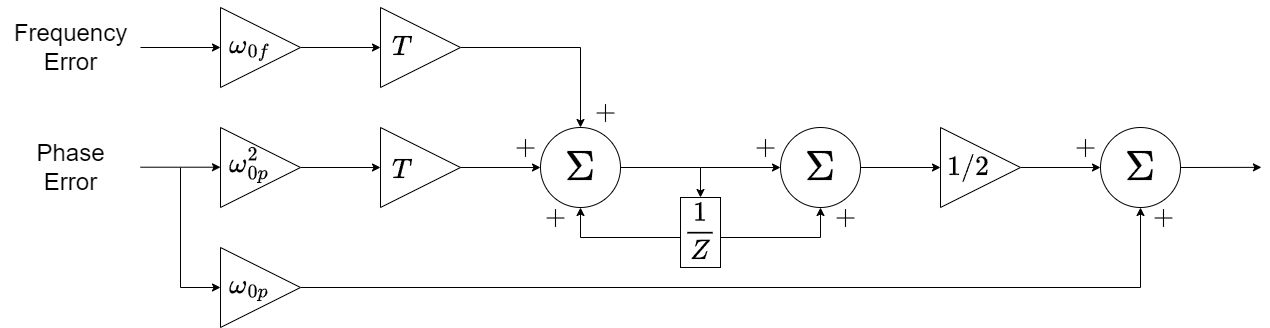
\includegraphics[width=\linewidth]{Figures/PLL.png}
    \caption{Discrete block diagram of the PLL-FLL loop filters used in this work.}
\end{figure}

The natural-radian frequency, \(\omega_0\), is set by the user, and common values for processing GPS L1 C/A exists in~\cite{kaplanUnderstandingGPSPrinciples2006}.

The DLL loop filter works in a similar fashion, but without the FLL loop filter assist and the addition of the output of the PLL-FLL loop filter to aid in replicating the true code phase (Figure~\ref{fig:DLL}).

\begin{figure}[!ht]\label{fig:DLL}
    \centering
    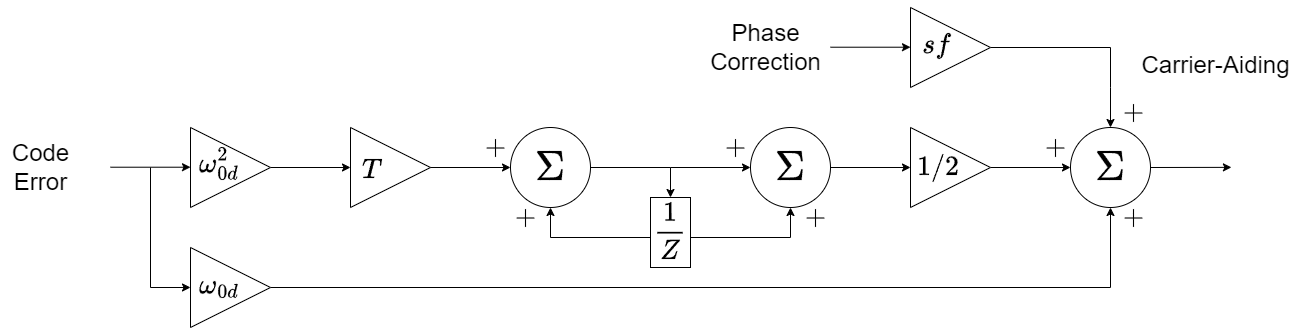
\includegraphics[width=\linewidth]{Figures/DLL.png}
    \caption{Discrete block diagram of the DLL loop filter used in this work.}
\end{figure}

In Figure~\ref{fig:DLL}, \(sf\) is known as the scale factor,
\begin{equation}\label{eq:sf}
    sf = \frac{R_c}{f_L},
\end{equation}

where \(R_c\) is the spreading (PRN) code rate, and \(f_L\) is the signal carrier frequency. For GPS L1 C/A, these are \(1.023 \times 10^6\) Hertz and \(1575.420 \times 10^6\) Hertz, respectively.

If the correlators, discriminators, and loop filters are correctly working in tandem, the replicated signal should accurately represent the received signal data and the receiver can decode the bits that translate to the broadcast navigation message from each satellite. A handful of subframes in the navigation message provide satellite ephemeris, or orbital parameters, that the receiver can use to propagate satellite PVT and determine its position through time.

\section{Navigation Algorithms}
Once the signal is accurately replicated and correctly decoded, the receiver begins to estimate a PVT solution. A position solution is found due to trilateration, meaning if there exists at least three unique ranges from known locations, then a position solution exists. Parallel to finding the position solution, receiver velocity can be found in the same way, using range rates in place of range. This sections describes calculating the ranges and range rates, and how they are used in the navigation processor for an estimated PVT solution.

\subsection{GPS Measurements}
There exists three main measurements from GPS satellites. The first of the three is pseudorange. By definition, it is the total time of transit from transmission to reception of the signal by the receiver. This value is then multiplied by the speed of light, providing this transit time in units of meters (Equation~\ref{eq:psr_time}).

\begin{equation}\label{eq:psr_time}
    \tilde{\rho}^j = (t_r - t_t^j)\,c
\end{equation}

In order to calculate a pseudorange, \(\rho \), from the \(j^{th}\) satellite The transmitted time of the signal, \(t_t\), is subtracted from the received time, \(t_r\), and then multiplied by the speed of light in vacuum, \(c\), as described before. For the rest of the work presented in this thesis, variables with \({\left(\;\tilde{}\;\right)}\) represent a measurement. The pseudorange from Equation~\ref{eq:psr_time} is a measurement because both the receiver clock and satellite clock have inherit biases and drifts that perturb their values from their truth. In addition to the errors in the clocks, the signal in space travels through the atmosphere, delaying the signal until it reaches the receiver. We can change Equation~\ref{eq:psr_time} such that these errors and delays are modeled. Describing the pseudorange in meters gives us,

\begin{equation}\label{eq:psr_meters}
    \tilde{\rho}^j = r_u^j + c\,t^j + c\,t_u + I^i_u + T^i_u+ M^i_u + \eta^i_{\rho},
\end{equation}
where,
\begin{equation}\label{eq:range_meters}
    r^j_u = \sqrt{{\left(x^j - x_u\right)}^2 + {\left(y^j - y_u\right)}^2 + {\left(z^j - z_u\right)}^2},
\end{equation}

\(t_u\) is the clock bias of the user, \(t^j\) is the clock bias of the \(j^{th}\) satellite, \(I\) is the ionospheric delay, \(T\) is the tropospheric delay, \(M\) is the delay of multipath, and \(\eta \) is additive Gaussian white noise all at time \(i\).

Positioning with GPS is possible because of the atomic clocks on board of each satellite. These clocks are highly stable and allow the Time of Week (TOW) to be transmitted in the data message for which the receiver decodes. Although the on board clocks are incredibly stable, the PRN sequence cannot be precisely transmitted at every millisecond. Fortunately, these clock errors are modeled in the data message, so \(t^j\) can be removed from the pseudorange equation. Clocks on board receivers are not quite as stable, and the received time of the signal is not known upon a cold start. A solution to this problem is initialize the received time to the first satellite transmit time and add a nominal offset of \(66.7\) milliseconds. This offset stems from a back of the envelope calculation based on the distance between MEO satellite orbits and the center of the Earth (Equation~\ref{eq:nominalOffset}).

\begin{equation}\label{eq:nominalOffset}
    {\left(t_u - t^{j} \right)}^{i = 0} = \frac{d_{MEO}}{c} \approx \frac{20000000}{299792458} \approx 0.0667
\end{equation}

The addition of the unknown receiver clock bias adds a fourth dimension to the trilateration position solution. This effectively requires that the receiver needs the ranges from four satellites to estimate \(x_u\), \(y_u\), \(z_u\), and \(t_u\).

The second measurement from GPS satellites is pseudorange-rate. By definition, pseudorange-rate is the measurement of the line of sight velocity that can be directly derived from changes in carrier frequency, also known as the Doppler frequency (Equation~\ref{eq:psrdot_time}).

\begin{equation}\label{eq:psrdot_time}
    \tilde{\dot{\rho}} = - \frac{\left(f_c - f_{IF}\right)\,c}{f_t}
\end{equation}

Above, \(f_c\) is the estimated frequency of the carrier wave, \(f_{IF}\) is the receiver intermediate frequency, and \(f_t\) is the nominal transmit frequency. Another way to represent pseudorange-rate measurement is by deriving Equation~\ref{eq:psr_meters} with respect to time. This geometric representation is seen in Equation~\ref{eq:psrdot_meters}.

\begin{equation}\label{eq:psrdot_meters}
    \tilde{\dot{\rho}} = \dot{r}_u^j + c\,\dot{t}_u + \dot{I}^i_u + \dot{T}^i_u + \eta^i_{\dot{\rho}}
\end{equation}

From Equation~\ref{eq:psrdot_meters}, it is assumed that the atomic clocks on board the satellites are stable enough such that the clock drift term is \(0\). The same can be said for \(\dot{M}^i_u\) where the error-rate due to multipath is miniscule.

Similar to the pseudorange measurement, if the receiver clock was perfect, only three satellites would be needed to measure pseudorange-rate. However, because of the instability in the receiver clock, the drift adds a bias to the frequencies. Therefore, four unique pseudorange-rates are still required in order to calculate receiver velocity.

The last measurement from GPS satellites is estimate of noise on a signal. The receiver utilizes a Carrier-to-Noise density ratio (\(C/N_0\)) to determine the quality of pseudorange and pseudorange-rate measurements from each satellite. Equation~\ref{eq:CN0} demonstrates how \(C/N_0\) is calculated in this work.

\begin{equation}\label{eq:CN0}
    \frac{C}{N_0} = 10\,\log_{10} {\left(\frac{\tilde{A} - 4\hat{\sigma_{eta}^2}}{2\,T\hat{\sigma_{eta}^2}}\right)}
\end{equation}

Where,

\begin{equation}\label{eq:ampitude}
    \tilde{A} = {\left(IE +IL\right)}^2 + {\left(QE + QL\right)}^2
\end{equation}

is the measured power of the accurately tracked signal using correlators defined in a previous section.\( \; \sigma_{\eta}^2\) is the variance in correlators that are the result of a shifting the replicated signal far outside of any correlation with the data of the received signal data. This work shifts these correlators by \(100\), \(200\), and \(300\) chips each~\cite{wattsGPSGLONASSL12019}. Furthermore, this variance is filtered with a moving average using a ratio of \(0.99:0.01\) between the current calculated variance and the previous filtered variance. Shifting the replicated signal by a large number of chips and then correlating the shifted signal with the received signal data is computationally expensive, but is necessary if using a Bayesian estimator or weighted least squares approach in both open-loop and vector tracking navigation algorithms.


\subsection{Open-Loop Architectures}
Open-loop architectures are navigation algorithms that provide no feedback to the tracking scheme described in the previous section. In benign, static and constant velocity scenarios, these algorithms still provide accurate PVT solutions and are critical for a closed-loop architecture like vector tracking to work properly. The following section covers Weighted Nonlinear Least Squares (WNLS), the method used to initialize the vector tracking algorithms in this work.

The state vector for receiver initialization comprises the position and velocities of the receiver in the Earth-Centered, Earth-Fixed (ECEF) frame, along with receiver clock bias and clock drift terms (Equation~\ref{eq:WLSstates})

\begin{equation}\label{eq:WLSstates}
    \hat{\mathbf{x}} =
    \begin{bmatrix}
        \hat{x}_u & \hat{\dot{x}}_u & \hat{y}_u & \hat{\dot{y}}_u & \hat{z}_u & \hat{\dot{z}}_u & c\hat{t}_u & c\hat{\dot{t}}_u \\
    \end{bmatrix}^T
\end{equation}

For the rest of the work presented in this thesis, variables with a \({\left(\;\hat{}\;\right)} \) represent an estimate of that variable. In Equation~\ref{eq:WLSstates}, \(T\) simply means the transpose of the array.

However, WNLS tries to estimate the errors between the true states and the estimated states (Equation~\ref{eq:errorStates}).

\begin{equation}\label{eq:errorStates}
    \delta\hat{\mathbf{x}} =
    \begin{bmatrix}
        \delta\hat{x}_u & \delta\hat{\dot{x}}_u & \delta\hat{y}_u & \delta\hat{\dot{y}}_u & \delta\hat{z}_u & \delta\hat{\dot{z}}_u & c\delta\hat{t}_u & c\delta\hat{\dot{t}}_u \\
    \end{bmatrix}^T
\end{equation}

These error states are then mapped to measurement residuals using the observation matrix, \(\mathbf{H}\) (Equation~\ref{eq:Hmat}).~\(\mathbf{H}\) is defined by the Jacobian of \(\mathbf{Y}\) with respect to \(\delta\hat{\mathbf{x}}\), or in a mathematical form,

\begin{equation}\label{eq:Jacobian}
    \mathbf{H} = \frac{\partial \mathbf{Y}}{\partial \delta\hat{\mathbf{x}}}.
\end{equation}

If we define \(\mathbf{Y}\) as
\begin{equation}\label{eq:Z}
    \mathbf{Y} =
    \begin{bmatrix}
        {\tilde{\rho}^1 - \hat{\rho}^1}\,, & {\tilde{\dot{\rho}}^1 - \hat{\dot{\rho}}^1}\,, & \hdots & {\tilde{\rho}^1 - \hat{\rho}^1}\, , & {\tilde{\dot{\rho}}^1 - \hat{\dot{\rho}}^1}
    \end{bmatrix}
\end{equation}

and then find the Jacobian of \(\mathbf{H}\), a relationship forms between the pseudoranges and pseudorange-rates and the ECEF position and velocity estimates of the receiver in the form of a unit vector (Equation~\ref{eq:unitVector}).

\begin{equation}\label{eq:unitVector}
    \mathbf{u}^j_{x,y,z} = \frac{\begin{bmatrix}
            x^j - x_u\, , & y^j - y_u\, , & z^j - z_u \\
        \end{bmatrix}
    }{r^j_u}
\end{equation}

Because the bias and drift of the clocks directly correspond to there error states, they are noted with a \(1\).

\begin{equation}\label{eq:Hmat}
    \mathbf{H} =
    \begin{bmatrix}
        -u_x^1 & 0      & -u_y^1 & 0      & -u_z^1 & 0      & 1      & 0      \\
        0      & -u_x^1 & 0      & -u_y^1 & 0      & -u_z^1 & 0      & 1      \\
        \vdots & \vdots & \vdots & \vdots & \vdots & \vdots & \vdots & \vdots \\
        -u_x^j & 0      & -u_y^j & 0      & -u_z^j & 0      & 1      & 0      \\
        0      & -u_x^j & 0      & -u_y^j & 0      & -u_z^j & 0      & 1      \\
    \end{bmatrix}
\end{equation}

The last piece in WNLS algorithm is defining the weights.\( \; \mathbf{W}\) is utilized by the algorithm to place more trust in satellites with a high \(C/N_0\) compared to satellites with lower \(C/N_0\). The weighting matrix is shown in Equation~\ref{eq:weights}.

\begin{equation}\label{eq:weights}
    \mathbf{W} = \begin{bmatrix}
        \sigma^2_{\rho^1} & 0                       & 0      & 0                 & 0                       \\
        0                 & \sigma^2_{\dot{\rho}^1} & 0      & 0                 & 0                       \\
        0                 & 0                       & \ddots & 0                 & 0                       \\
        0                 & 0                       & 0      & \sigma^2_{\rho^j} & 0                       \\
        0                 & 0                       & 0      & 0                 & \sigma^2_{\dot{\rho}^j} \\
    \end{bmatrix}^{-1}
\end{equation}

Where
\begin{equation}\label{eq:psrVar}
    \sigma^2_{\rho^j} = \frac{\lambda^2_{code}}{2T^2{\left(\frac{C}{N_0}^2\right)}} + \frac{\lambda^2_{code}}{4T\frac{C}{N_0}}
\end{equation}

is the variance of the pseudorange measurement from the \(j^{th}\) satellite and

\begin{equation}\label{eq:psrdotvar}
    \sigma^2_{\dot{\rho}^j} = {\left(\frac{\lambda_{carrier}}{\pi T}\right)}^2\,{\left(\frac{2}{T^2{\left(\frac{C}{N_0}^2\right)}} + \frac{2}{T \frac{C}{N_0}}\right)}
\end{equation}

is the variance of the pseudorange-rate measurement from the \(j^{th}\) satellite. In Equations~\ref{eq:psrVar} and~\ref{eq:psrdotvar}, \(\lambda_{code}\) is the wavelength of data signal and \(\lambda_{carrier}\) is the wavelength of the carrier signal. In this case, \(C/N_0\) is specified in dB-Hz.

Once the above matrices are created, the WNLS algorithm (Equation~\ref{eq:wnls}) can be performed iteratively until the magnitude of the error state vector is small, meaning the algorithm has converged.

\begin{equation}\label{eq:wnls}
    \delta\hat{\mathbf{x}} = {{\left(\mathbf{H}^{T}\mathbf{W}\mathbf{H}\right)}^{-1}\,\mathbf{W}\mathbf{Y}}
\end{equation}

Once an initial receiver position has been found, vector tracking channels can open and a closed form PVT solution can start to be processed. Vector tracking loops and algorithms are discussed in the next chapter.

\section{Conclusions}
The architecture of a scalar-tracking software defined received was explained. For more information on any of the subsections discussed in this chapter, detailed descriptions of each can be found in the literature. Because the focus of this thesis is vector tracking, the meaning of this chapter was to provide the reader with a fundamental understanding of tracking loops that will be expanded on further in the next chapter.
\chapter{\textbf{Proposed Navigation Filter Architecture}}
Scalar tracking loops discussed in Chapter~3 are critically important to receivers as they adapt the replica signal to match the received signal data for proper decoding. However, traditional scalar loop filters assume a static noise bandwidth, regardless of receiver or satellite dynamics. If either platforms have unmodeled dynamics, these static bandwidths can permit too much noise into the navigation solution, or neglect some of the dynamics by filtering too much of the signal. One solution to this problem is implementing an adaptive Kalman filter to optimally select bandwidths~\cite{huangIntegratedAdaptiveKalman2019}. In this implementation, the Kalman filter estimates the proper bandwidth based on discriminator residuals and modeled variances, but is agnostic to the dynamics of the receiver or the satellite dynamics. The addition of an adaptive Kalman filter is an improvement, but leaves a lot to be desired as each channel is still being tracked individually, resulting in low-powered channels having a high likelihood of being lost.

Another, more optimal, solution is to estimate the local replica signal from receiver and satellite dynamics at every integration period. This requires an updated estimate of the navigation solution at every integration period. This approach combines the adaptive bandwidth from~\cite{huangIntegratedAdaptiveKalman2019} along with knowledge of the receiver and satellite dynamics stemming from the navigation solution. This closed-loop approach is known as {vector tracking} and will be discussed in greater detail later on in this chapter. Specifically, the Vector Delay and Frequency Lock Loop (VDFLL) is the vector tracking implementation used in this thesis.

To build on the attractive approach that vector tracking brings to processing received signal data, the novelty of this work proposes an addendum to the existing navigation filter architecture by adding a FVDM to predict the trajectory of flight vehicle to better assist with the processing of the signal. When coupling external propagation schemes to GPS measurements, there are three common regimes.

The simplest form is loosely-coupled, where receiver position and velocity measurements are coupled with the predicted states from the external sensor to provide an improved receiver state estimate (Figure~\ref{fig:LC}). The advantages of loose coupling is that the GPS receiver does not need to be modeled extensively; however, the noise provided by the receiver is not white, making the Kalman filter sub-optimal~\cite{lashleyPerformanceAnalysisVector2009}. Furthermore, a {loosely-coupled} architecture only works with at least 4 satellites are transmitting to the receiver {--} which is not always the case for GPS-challenged environments~\cite{grovesPrinciplesGNSSInertial2012}.

\begin{figure}[!ht]
    \centering
    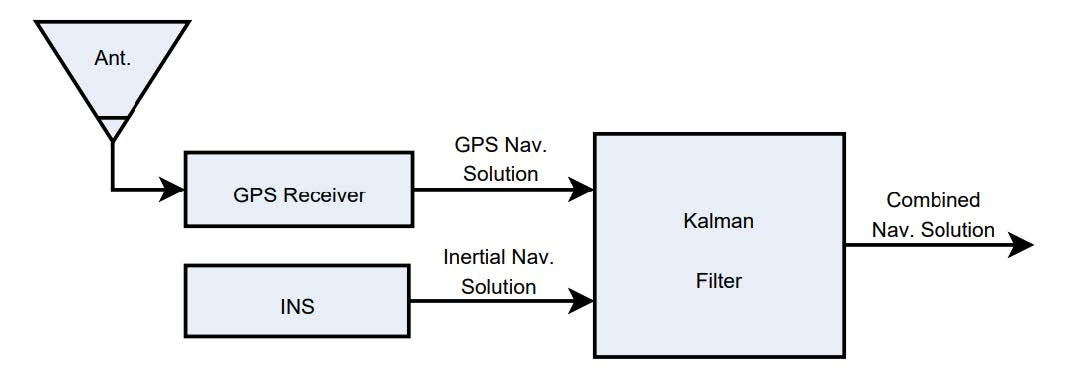
\includegraphics[width=\linewidth]{Figures/LC.jpg}
    \caption{Loosely-coupled architecture between GPS and INS systems~\cite{hammAnalysisSimulatedPerformance2005}.}\label{fig:LC}
\end{figure}

A more complicated coupling is {tightly-coupled}, where the navigation filter receives raw pseudorange and pseudorange rate measurements from the GPS receiver~\cite{kaplanUnderstandingGPSPrinciples2006} (Figure~\ref{fig:TC}). Because of this, tightly-coupled systems are still able to perform with less than 4 satellites, for a limited time. The draw back to tightly-coupled navigation architectures is the complexity of implementation. However, a working tightly-coupled system provides generous improvements over loosely-coupled frameworks, especially in GPS-challenged environments~\cite{grierPositionNavigationTiming}.

\begin{figure}[!ht]
    \centering
    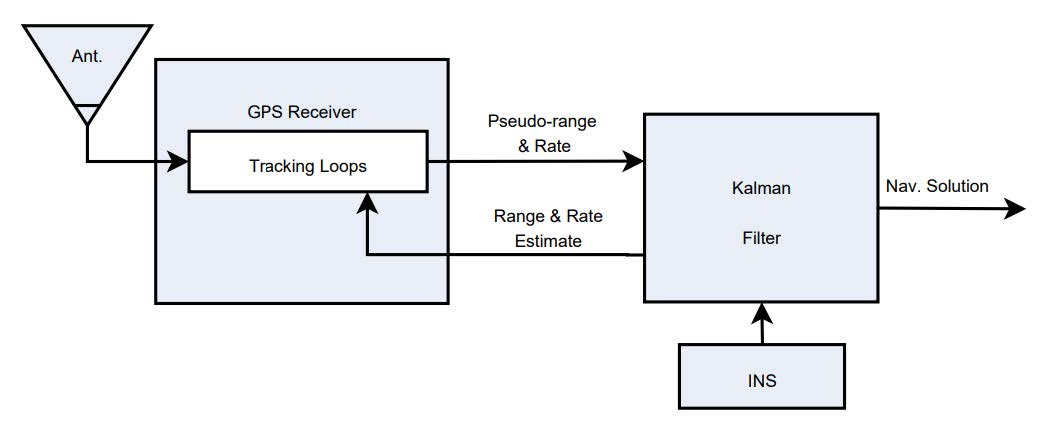
\includegraphics[width=\linewidth]{Figures/TC.jpg}
    \caption{Tightly-coupled architecture between GPS and INS systems~\cite{hammAnalysisSimulatedPerformance2005}.}\label{fig:TC}
\end{figure}

{Deeply-coupled}, or ultra-tight coupling, is the last of the common methods to couple external state predictions to GPS measurements. The downsides to deeply integrating an external sensor or vehicle dynamic model to GPS measurements is increased complexity and the reliance on the receiver to know its position beforehand {--} as is common with vector tracking. Generally, a deeply integrated system revolves around adapting the EKF that exists for a vector tracking architecture and appending the external dynamic model. This way, the GPS receiver and the added dynamic model are tied together at the most basic level. The benefits of a complete deeply-coupled system allow continued tracking of a degraded signal \(2-6\) dB higher than their true carrier-to-noise ratios~\cite{wattsGPSGLONASSL12019}. Furthermore, the addition of external dynamics allows better predictions of receiver pose due to the navigation filter acknowledging the dynamics of the collection platform. This is especially beneficial for high-dynamic vehicles such as hyper-velocity aircraft~\cite{pozzobonSupersonicGNSSAuthentication2014} or vehicles in GPS-challenged environments~\cite{martinGPSCarrierPhase2017}. For these benefits, a deep integration of the FVDM with GPS correlator-level measurements is the focus of this work.

\section{\textbf{Vector Delay and Frequency Lock Loop}}
Vector tracking first utilized a Vector Delay Lock Loop (VDLL) and was proposed by~\cite{e.m.coppsOptimalProcessingGPS1980}. In a VDLL\@, the EKF provides continuous estimates of the code frequency, updating the DLL, improving overall tracking performance. Later on,~\cite{bradfordparkinsonGlobalPositioningSystem1996}, explores tracking both code frequency and carrier frequency in an EKF, coined the VDFLL\@. This method showed great improvements over scalar tracking algorithms and moderate improvements over the VDLL\@. The VDFLL proves best when tracking weaker GNSS signals under high dynamic stress~\cite{lashleyPerformanceAnalysisVector2009}. Furthermore, recent analyses from~\cite{ziedanMultipathChannelEstimation2012} prove the VDFLL has improved resilience to multipath delay as well. A block diagram of the VDFLL is shown in Figure~\ref{fig:VDFLL}.

\begin{figure}[!ht]
    \centering
    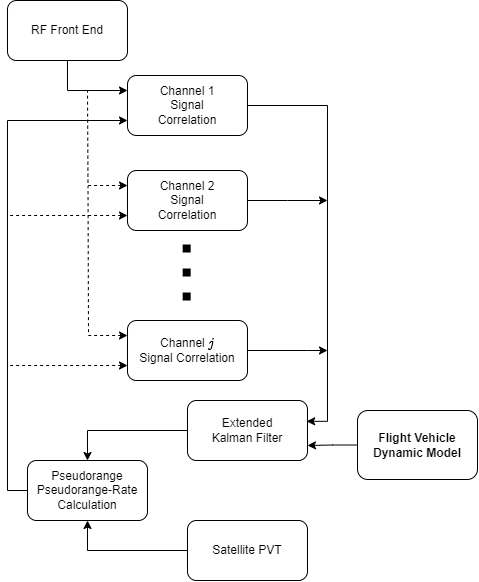
\includegraphics[width=0.45\linewidth]{Figures/VectorTracking.drawio.png}
    \caption{Block diagram of the VDFLL used in this work (Adapted from~\cite{grierPositionNavigationTiming}).}\label{fig:VDFLL}
\end{figure}

From Figure~\ref{fig:VDFLL}, the \textit{RF Front End} block refers to the discussion in Section~3.1. The signal correlation blocks represent Equation~\ref{eq:correlators} and also the the FLL and DLL discriminators specified in Equations~\ref{eq:FLLdisc} and~\ref{eq:DLLdisc}, respectively. The basic flow of the VDFLL requires the receiver to know its position and the positions of the satellites \textit{a priori}. Preferably, initial positions and satellite positions that are fed into the VDFLL are from processing the received signal for a length of time required to decode the navigation message using an open-loop architecture like the scalar tracking loops and WNLS discussed in Chapter 3. The measurement inputs of the EKF in Figure~\ref{fig:VDFLL} are residual pseudorange and pseudorange-rates in the form of discriminator outputs. The EKF uses the measurements from the current signal correlations to directly estimate the pose of the receiver. Using the ephemeris of the satellites and the corrected position estimates, new code phase and carrier frequency estimates are generated for the next integration period. To improve the estimated position from the EKF, the FVDM is used as the process model to propagate the non-linear motion of the aircraft in time. The next section covers the time update and measurement update within the EKF\@.

\section{\textbf{Deeply Coupled GPS and FVDM Navigation Filter}}
As stated previously, the VDFLL replaces the scalar DLLs and FLLs with a single EKF\@. This sections describes the design of the EKF for the proposed navigation filter. The EKF for this work represents a position-state filter where the state vector is defined by Equation~\ref{eq:stateVector}.

\begin{equation}\label{eq:stateVector}
    \mathbf{X} =
    \begin{bmatrix}
        \mathbf{X}_V & \mathbf{X}_{\omega} & \mathbf{X}_P & \mathbf{X}_{\psi} & \mathbf{X}_t \\
    \end{bmatrix}^T
\end{equation}

The essential elements for the state vector are sectioned into five terms.~\(\mathbf{X}_V\) (Equation~\ref{eq:velVector}) describes the velocity states of the aircraft from Earth to body with respect to the Local Navigation frame.

\begin{equation}\label{eq:velVector}
    \mathbf{X}_V =
    \begin{bmatrix}
        V_N & V_E & V_D \\
    \end{bmatrix}
\end{equation}

The angular rates (\(\mathbf{X}_{\omega}\)) are represented from inertial to body with respect to the body frame (Equation~\ref{eq:omegaVector}).

\begin{equation}\label{eq:omegaVector}
    \mathbf{X}_{\omega} =
    \begin{bmatrix}
        p_{ib}^b & q_{ib}^b & r_{ib}^b \\
    \end{bmatrix}
\end{equation}

The position estimates of the aircraft are from Earth to body with respect to the Local Navigation frame (Equation~\ref{eq:posVector}), similar to the velocity states.

\begin{equation}\label{eq:posVector}
    \mathbf{X}_P =
    \begin{bmatrix}
        \lambda_{eb}^n & L_{eb}^n & h_{eb}^n \\
    \end{bmatrix}
\end{equation}

Equation~\ref{eq:eulVector} represents the Euler angles of the aircraft, represented from body to the local navigation frame.

\begin{equation}\label{eq:eulVector}
    \mathbf{X}_{\psi} =
    \begin{bmatrix}
        \phi_{bn} & \theta_{bn} & \psi_{bn} \\
    \end{bmatrix}
\end{equation}

Completing the state vector are the clock terms that represent estimates of the clock bias and clock drift of the receiver during flight (Equation~\ref{eq:clkVector}). The clock bias and clock drift are scaled by the speed of light (\(c\)) to give them units of meters and meters/second, respectively.

\begin{equation}\label{eq:clkVector}
    \mathbf{X}_t = \begin{bmatrix}
        c\delta t & c\delta\dot{t} \\
    \end{bmatrix}
\end{equation}

The dynamics of the aircraft are defined by

\begin{equation}\label{eq:eulerIntegration}
    \dot{\mathbf{X}} = F\left(\mathbf{X},f_{ib}^b,M_{ib}^b\right) + \mathbf{B}_{dyn}w_{dyn} + \mathbf{B}_{clk}w_{clk},
\end{equation}

where \(\mathbf{B}_{dyn}\) is the noise distribution matrix related to the dynamics (Equation~\ref{eq:Bdyn}).

\begin{equation}\label{eq:Bdyn}
    \mathbf{B}_{dyn} =\begin{bmatrix}
        \mathbf{I}_{6,6} & \mathbf{0}_{6,2} \\
        \mathbf{0}_{8,6} & \mathbf{0}_{8,2} \\
    \end{bmatrix}_{14,8}
\end{equation}

\(w_{dyn}\) is the disturbance vector for the aircraft dynamics, as shown in Equation~\ref{eq:wDyn}. Equation~\ref{eq:Bdyn} shows that only the linear and angular accelerations are affected by the disturbances, but these errors trickle down into the kinematic equations for the position and Euler derivatives.

\begin{equation}\label{eq:wDyn}
    w_{dyn} = \begin{bmatrix}
        \sigma^2_{V_N} & \sigma^2_{V_E} & \sigma^2_{V_E} & \sigma^2_{p} & \sigma^2_{q} & \sigma^2_{r}
    \end{bmatrix}^T
\end{equation}

\(\mathbf{B}_{clk}\) and \(w_{clk}\) are the noise distribution matrices (Equation~\ref{eq:Bclk}) and clock variance vector (Equation~\ref{eq:wClk}), respectively.

\begin{equation}\label{eq:Bclk}
    \mathbf{B}_{clk} =\begin{bmatrix}
        \mathbf{0}_{6,6} & \mathbf{0}_{12,2} \\
        \mathbf{0}_{8,6} & -\mathbf{I}_{2,2} \\
    \end{bmatrix}_{14,8}
\end{equation}

\begin{equation}\label{eq:wClk}
    w_{clk} = \begin{bmatrix}
        \sigma^2_b & \sigma^2_d \\
    \end{bmatrix}^T
\end{equation}

\(\sigma^2_b\) and \(\sigma^2_d\) are modeled variances based on the clock embedded into the receiver. For the receiver simulated in this work, an Oven Controlled Crystal Oscillator (OCXO) is used. More information on calculating the clock variance based on oscillator type can be found in~\cite{robertgroverbrownIntroductionRandomSignals2013}.

\(F\) is a set of non-linear equations that define the motion of the aircraft as a function of the current state in time (\(\mathbf{X}\)), the forces in the body frame (\(f_{ib}^b\)) and the moments about the body frame (\(M_{ib}^b\)). Calculation of the forces and moments were discussed in Chapter 2.

Calculations of the forces and moments and moments must be done in the body frame. Rotating all of the equations that build the total forces and moments acting onto the airframe into a global or local navigation reference frame would be cumbersome and introduce more complexity than necessary. However, because of the measurements generated from the correlators and discriminators are composed in the ECEF reference frame, the FVDM must be propagated with respect to the curvature of the Earth in a global frame. For this work, the equations of motion are rotated into the local navigation frame.

The state derivatives of the velocity components are defined in Equation~\ref{eq:acc}.

\begin{equation}\label{eq:acc}
    \begin{bmatrix}
        \dot{V_N} \\
        \dot{V_E} \\
        \dot{V_D} \\
    \end{bmatrix} =
    \mathbf{C}_{b}^{n}\frac{\mathbf{f}_{ib}^b}{m} - \left(2\mathbf{\Omega}_{ie}^n - \mathbf{\Omega}_{en}^n\right)
    \begin{bmatrix}
        V_N \\
        V_E \\
        V_D \\
    \end{bmatrix}
\end{equation}

The first term above represents the forces acting onto the airframe with respect to the body frame divided by the mass of aircraft, \(m\). For the purposes of this work, the mass of the aircraft is assumed constant. This specific force vector is rotated into the local navigation frame using \(\mathbf{C}_b^n\), defined in Equation~\ref{eq:ECEF2LNDCM}. The latter term in Equation~\ref{eq:acc} represents the rotation rate (Equation~\ref{eq:earthrotation}) of the Earth in skew-symmetric form and the transport rate (Equation~\ref{eq:transportrate}) in skew-symmetric form, both rotated into the local navigation frame and multiplied by the current velocity of the aircraft.

\begin{equation}\label{eq:earthrotation}
    \mathbf{\Omega}_{ie}^n =
    \omega_{ie}\begin{bmatrix}
        0                          & \sin\left(L_{eb}^n\right) & 0                          \\
        -\sin\left(L_{eb}^n\right) & 0                         & -\cos\left(L_{eb}^n\right) \\
        0                          & \cos\left(L_{eb}^n\right) & 0                          \\
    \end{bmatrix}
\end{equation}

Where \(\omega_{ie}\) is \(7.27\times10^{-5}\) radians/second.

\begin{equation}\label{eq:transportrate}
    \mathbf{\Omega}_{en}^n = \begin{bmatrix}
        0                & -\omega_{en,z}^n & -\omega_{en,y}^n \\
        \omega_{en,z}^n  & 0                & -\omega_{en,x}^n \\
        -\omega_{en,y}^n & \omega_{en,x}^n  & 0                \\
    \end{bmatrix}
\end{equation}

Where

\begin{equation}\label{eq:omega_en_n}
    \omega_{en}^n =
    \begin{bmatrix}
        V_E/(R_E + h_{eb}^n)               \\
        -V_N/(R_N + h_{eb}^n)              \\
        V_E\tan(L_{eb}^n)/(R_E + h_{eb}^n) \\
    \end{bmatrix}
\end{equation}

Above, \(R_E\) and \(R_N\) refer to the meridian and transverse radii of curvature as described in Equations~\ref{eq:meridiancurvature} and~\ref{eq:transversecurvature}, respectively.

The derivatives of the angular rates are defined as

\begin{equation}\label{eq:angacc}
    \begin{bmatrix}
        \dot{p}_{ib}^b \\
        \dot{q}_{ib}^b \\
        \dot{r}_{ib}^b \\
    \end{bmatrix} =
    {\mathbf{I}_{cg}^b}^{-1}\left[\mathbf{M}_{ib}^b -
        \begin{bmatrix}
            p \\
            q \\
            r \\
        \end{bmatrix} \times
        \left(\mathbf{I}_{cg}^b
        \begin{bmatrix}
            p \\
            q \\
            r \\
        \end{bmatrix}
        \right)
        \right],
\end{equation}
where \(\mathbf{I}_{cg}^b\) are the mass moments of inertia for the aircraft. For the purpose of this work, the aircraft is modelled symmetrically about each of the axes such that \(\mathbf{I}_{cg}^b\) only has terms along the diagonal.

The local navigation frame position derivatives are described by Equation~\ref{eq:posrate}.
\begin{equation}\label{eq:posrate}
    \begin{bmatrix}
        \dot{\lambda}_{eb}^n \\
        \dot{L}_{eb}^n       \\
        \dot{h}_{eb}^n       \\
    \end{bmatrix} =
    \begin{bmatrix}
        \frac{V_N}{R_N + h_{eb}^n}                                       \\
        \frac{V_E}{\left(R_E + h_{eb}^n\right)\cos\left(L_{eb}^n\right)} \\
        -V_D                                                             \\
    \end{bmatrix}\\
\end{equation}

The derivatives of the Euler angles are seen in Equation~\ref{eq:eulerRates}

\begin{equation}\label{eq:eulerRates}
    \begin{bmatrix}
        \dot{\phi}_{bn}   \\
        \dot{\theta}_{bn} \\
        \dot{\psi}_{bn}   \\
    \end{bmatrix} =
    \mathbf{C}_{\omega}
    \left(
    \begin{bmatrix}
            p \\
            q \\
            r \\
        \end{bmatrix} -
    \mathbf{C_n^b}\left(\omega_{ie}^n + \omega_{en}^n\right)
    \right)
\end{equation}

Calculation of the Euler rates is the difference between the current angular rates of the aircraft and the rotation of the Earth along with the transport rate, similar to the calculation of linear acceleration in Equation~\ref{eq:acc}. This difference is rotated by \(\mathbf{C}_{\omega}\) defined by Equation~\ref{eq:cOmega}.

\begin{equation}\label{eq:cOmega}
    \mathbf{C}_{\omega} =
    \begin{bmatrix}
        1 & \tan(\theta)\sin(\theta)    & \tan(\theta)\cos(\phi)      \\
        0 & \cos(\phi)                  & -\sin(\phi)                 \\
        0 & {\sin(\phi)}/{\cos(\theta)} & {\cos(\phi)}/{\cos(\theta)} \\
    \end{bmatrix}
\end{equation}

The last of the state derivatives are the clock terms. Both the clock drift and clock drift rate are scaled by the speed of light to give them units of \( m \, s^{-1}\) and \( m \, s^{-2}\).

\begin{equation}\label{eq:clkRates}
    \begin{bmatrix}
        c\delta \dot{t} \\
        c\delta\ddot{t} \\
    \end{bmatrix} =
    \begin{bmatrix}
        0 & 1 \\
        0 & 0 \\
    \end{bmatrix}
    \begin{bmatrix}
        c\delta {t}    \\
        c\delta\dot{t} \\
    \end{bmatrix}
\end{equation}

Once the state derivatives are calculated using the aforementioned equations of motions, they are integrated using Euler integrations to propagate the states forward in time. This provides the EKF with the predicted states for the current time step.

The other part of the prediction step in the EKF is the formation of the predicted covariance matrix \(\mathbf{P}^-_{k}\). This is defined by Equation~\ref{eq:pminus}.

\begin{equation}\label{eq:pminus}
    \mathbf{P}^-_{k} = \mathbf{\Phi}\mathbf{P}^-_{k-1} \mathbf{\Phi}^T + \mathbf{Q_d}
\end{equation}

\( \mathbf{\Phi}\) is defined as the state transition matrix. The state transition matrix is composed of \(\mathbf{X}\) and the relationship with each state derivative \( \dot{\mathbf{X}}\). This done by taking the Jacobian and is represented by Equation~\ref{eq:stateJacobian}.

\begin{equation}\label{eq:stateJacobian}
    \mathbf{J} = \frac{\partial \dot{\mathbf{X}}_{14,1}}{\partial \mathbf{X}_{14,1}}
\end{equation}

The evaluated Jacobian, \(\mathbf{J}\), is a square 14 row, 14 column matrix that varies as function of the forces and moments in time. These forces and moments can vary based on the disturbances and the controls inputs, so \(\mathbf{J}\) must be evaluated at every time step. Because of the complexity of the Jacobian, it is solved using the symbolic toolbox in MATLAB\@.

The state propagation is continuous, but \(\mathbf{\Phi}\) is discrete. This means that the Jacobian must be discretized. The discretization of the Jacobian from continuous to discrete is introduced by Equation~\ref{eq:Phi}

\begin{equation}\label{eq:Phi}
    \mathbf{\Phi} = \textrm{expm}(\mathbf{J}\Delta t)
\end{equation}

The discrete process noise covariance (\(\mathbf{Q}_d\)) encapsulates the disturbances onto the aircraft dynamics such that the EKF can better correct the states during the measurement update. To transform the process noise from continuous to discrete, Equation~\ref{eq:Qd} is used.

\begin{equation}\label{eq:Qd}
    \mathbf{Q_d} = \mathbf{\Phi}\mathbf{B}_w \left(ww^T\right) \mathbf{B}_w^T \mathbf{\Phi}^T \Delta t
\end{equation}

Above, \(\mathbf{B}_w\) is the noise distribution matrix that is augmented with \(\mathbf{B}_{dyn}\) and \(\mathbf{B}_{clk}\).~\(w\) is the disturbance vector and is formed by concatenating the dynamic state disturbances and the clock term disturbances together (Equation~\ref{eq:w}). For the work presented in this thesis, the time step (\(\Delta t\)) is \(200\) Hertz.

\begin{equation}\label{eq:w}
    w = \begin{bmatrix}
        w_{dyn} & w_{clk}
    \end{bmatrix}
\end{equation}

Once the state and covariance prediction are calculated, the \textit{a priori} part of the EKF is complete. The EKF will continue to predict the state and covariance until measurements from the vector tracking receiver are available. The next subsection covers the measurement update of the EKF, correcting the predicted covariance and predicted states.

\subsection{\textbf{Update \textit{a posteriori}}}
The measurement update in the EKF utilizes the current predicted covariance and measurement covariance to optimally correct the predicted states and predicted covariance. Equation~\ref{eq:L} shows the calculation of the Kalman gain.

\begin{equation}\label{eq:L}
    \mathbf{K}_k = \mathbf{P}^-_k \mathbf{H}^T_k{\left(\mathbf{H}_k\mathbf{P}^-_k\mathbf{H}^T_k + \mathbf{R}_k\right)}^{-1}
\end{equation}

The Kalman gain, \(\mathbf{K}\), is a function of the observation matrix, \(\mathbf{H}\), measurement covariance matrix, \(\mathbf{R}\), and the predicted covariance, described previously. The observation matrix maps the residual pseudorange and pseudorange rates to the local navigation states. This is demonstrated by Equation~\ref{eq:H}.

\begin{equation}\label{eq:H}
    \mathbf{H}_k = \begin{bmatrix}
        \mathbf{u}^{n,j}_{1,3} & \mathbf{0}_{1,3} & \mathbf{0}_{1,3}            & 0                & 0  & -1 \\
        \mathbf{0}_{1,3}       & \mathbf{0}_{1,3} & \mathbf{h}^j_{\rho p_{1,3}} & \mathbf{0}_{1,3} & -1 & 0  \\
    \end{bmatrix}_{2j,14}
\end{equation}

Using the predicted estimate of the receiver position Euler attitude, \(\mathbf{H}\) rotates the ECEF residuals to the local navigation frame. There are arrays of zeros where the measurements do not correlate to the corresponding states. The rotation of the unit vectors from ECEF to the local navigation frame is shown by Equation~\ref{eq:nav_u} and the rotation for the position measurements is given by Equation~\ref{eq:nav_h}.

\begin{equation}\label{eq:nav_u}
    \mathbf{u}^{n,j} = \mathbf{C}_e^n \mathbf{u}^{e,j}
\end{equation}

\begin{equation}\label{eq:nav_h}
    \mathbf{h}^j_{\rho p} =
    \begin{bmatrix}
        \left(R_N + h^n_{eb}\right)\mathbf{u}^{n,j}_N               \\
        \left(R_E + h_{eb}^n\right)\cos(L^n_{eb})\mathbf{u}^{n,j}_E \\
        -\mathbf{u}^{n,j}_D                                         \\
    \end{bmatrix}
\end{equation}

The measurement covariance matrix,~\(\mathbf{R}\), was described as the weighting matrix, \(\mathbf{W}\), in Chapter 3. The variances of the measurements are still calculated as a function of the carrier-to-noise ratio. Once the Kalman gain is calculated for the current time step, it can be used with the measurement vector, \(\Delta z\), to update the predicted state estimate (Equation~\ref{eq:deltaZ} and~\ref{eq:xplus}).

\begin{equation}\label{eq:deltaZ}
    \Delta z = \begin{bmatrix}
        \Delta\dot{\rho}^{\,1} & \Delta{\rho}^{\,1} & \hdots & \Delta\dot{\rho}^{\,j} & \Delta{\rho}^{\,j} \\
    \end{bmatrix}^T
\end{equation}

\begin{equation}\label{eq:xplus}
    \mathbf{X}_k^+ = \mathbf{X}^-_k + \mathbf{K}_k\Delta Z
\end{equation}

The last step in the measurement update is correcting the predicted covariance (Equation~\ref{eq:pplus}). The predicted covariance will drift based on the process noise covariance matrix and correcting the covariance by using the newly calculated Kalman gain will inform the filter of the confidence in the process model.

\begin{equation}\label{eq:pplus}
    \mathbf{P}^+_k = \left(\mathbf{I} - \mathbf{K}_k\mathbf{H}_k\right)\mathbf{P}^-_k
\end{equation}

After the measurement update of the EKF is complete, the estimated states and covariance matrices redefine the predicted state and covariances, closing the loop in the proposed navigation filter.

\section{\textbf{Conclusions}}
Vector tracking is a closed loop solution to estimating navigation states in a GPS receiver. The proposed navigation filter augments the existing VDFLL architecture by instantiating the FVDM as the process model in the EKF\@. This chapter covered the differences between scalar and vector tracking loops and expanded on the utilization of the FVDM to propagates the states of aircraft while also using correlator-level GPS measurements to correct the states and maintain channel lock for the duration of the simulations. This chapter provided a general overview of the VDFLL and covered the additions to the VDFLL architecture that did not exist before. For a more nuanced implementation of the VDFLL, the reader is asked to read the sources cited throughout the chapter for more information.
\chapter{\textbf{Simulation Environment}}
 Up until this point, this thesis has covered the navigation architecture in the overarching Guidance, Navigation, and Control (GNC) flight vehicle model. This chapter will expand on both the guidance and control architecture utilized for this work. Although these are not the primary focus of this thesis, they are important to discuss if others wish to replicate the study.

\section{\textbf{Guidance System}}
The guidance system for a flight vehicle holds responsibility for providing reference points to the controllers that provide actuation of the control surfaces and engine controls. These reference points are a function of various flight conditions including the atmospheric conditions, estimated pose of the aircraft, and engine efficiency. For the purposes of this work, the primary goal of the guidance system is to accept a user-defined trajectory consisting of waypoints defined in the local navigation frame and convert these into aircraft heading, pitch, throttle, and propeller pitch reference commands for the controllers to interpret. The following subsection provides an overview of creating trajectories for the guidance system.

\subsection{\textbf{Waypoint Generation}}
In this work, the generation of waypoints is a simple process where the user manually picks a trajectory using Google Earth~\cite{GoogleEarth1969}. Once a trajectory is created (Figure~\ref{fig:googleEarth}) and saved as a \textit{kml} file, it can be brought into MATLAB and converted into a matrix of values in the local navigation frame. Note, at this point, it may be beneficial to alter the altitude values such that the aircraft climbs, descends, or maintains a certain altitude during the length of the simulation. The conversion of the \textit{kml} file can be done using the \textit{KML Toolbox} from~\cite{KMLToolboxFile1969}.

\begin{figure}[!ht]
    \centering
    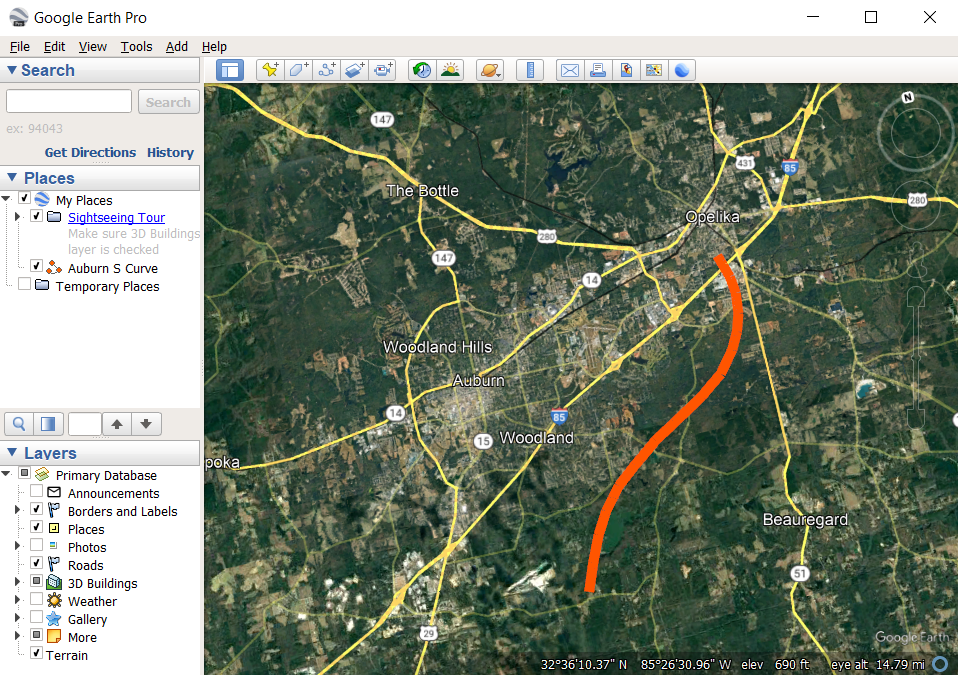
\includegraphics[width=0.75\linewidth]{Figures/auburnScurve.png}
    \caption{A custom trajectory created in Google Earth for the guidance system discussed in this work.}\label{fig:googleEarth}
\end{figure}

Once the trajectory is imported into the model, it is used within the guidance system to produce reference commands of desired heading, pitch, throttle, and propeller pitch. This work uses the \textit{uavWaypointFollower} class provided by the UAV Toolbox in MATLAB\@. Other methods of waypoint following can be used, as long as they output the aforementioned reference commands.

The waypoint follower calculates the reference heading and pitch by using trigonometric relationships between the flight vehicles current pose and the selected waypoints position. The throttle is chosen such that time between waypoints is consistent. The propeller pitch is controlled such that propeller efficiency is maximized (Equation~\ref{eq:propellerefficiency}). These reference commands are passed to the control law, mapping commanded values to normalized aircraft stick movements, throttle lever position, and propeller lever position. This processed in discussed in the next section.

\section{\textbf{Control Scheme}}

As stated previously, the guidance system and control law are not the primary focus of this work. Because of this, classical Proportional-Integral-Derivative (PID) controllers are used to actuate the controls surfaces to the desired values from the guidance system. During simulations presented for this thesis, only four of the available eleven inputs are being controlled to maintain the desired trajectory of the aircraft. Table~\ref{tbl:controls} lays out the available inputs available for the Diamond-DA40 modeled in this work.

\begin{table}[!ht]
    \caption{List of available, controllable inputs to the Diamond DA40 modeled in this thesis.}\label{tbl:controls}
    \centering
    \begin{tabular}{llc}
        \toprule
        \textbf{Input}     & \textbf{Definition}                                               & \textbf{Controlled} \\
        \midrule
        Lateral Stick      & L/R movement of pilot stick, maps to \(\delta_a\)                 & \(X\)               \\
        Longitudinal Stick & Fwd/Aft movement of pilot stick, maps to \(\delta_e\)             & \(X\)               \\
        Rudder Pedals      & In/Out position of left/right rudder pedals, maps to \(\delta_r\) &                     \\
        Throttle Lever     & Lever \% w.r.t.\ throttle, maps to engine RPM                     & \(X\)               \\
        Propeller Lever    & Lever \% w.r.t.\ propeller pitch normal to freestream             & \(X\)               \\
        Mixture Lever      & Lever \% w.r.t.\ fuel-to-air ratio within engine                  &                     \\
        Left Brake         & Position of L rudder pedal when a/c is on ground                  &                     \\
        Right Brake        & Position of R rudder pedal when a/c is on ground                  &                     \\
        Aileron Trim       & \(\delta_a\) needed to maintain a/c stability                     &                     \\
        Rudder Trim        & \(\delta_r\) needed to maintain a/c stability                     &                     \\
        Elevator Trim      & \(\delta_e\) needed to maintain a/c stability                     &                     \\
        \bottomrule
    \end{tabular}
\end{table}

Control of the lateral stick is a function of two closed-loop controllers based on the commanded heading from the guidance system and the current heading and roll angle of the aircraft. It is assumed that the nose of the aircraft always points in the direction of the aircraft's velocity. Figure~\ref{fig:latstickcontrol} shows the two closed-loop controllers working in series with their listed gains for more detail.

\begin{figure}[!ht]
    \centering
    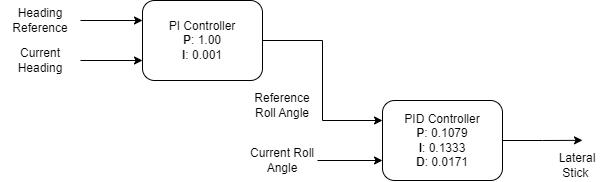
\includegraphics[width=0.75\linewidth]{Figures/latstickcontrol.drawio.png}
    \caption{Block diagram of lateral stick control through two closed-loop, PID controllers.}\label{fig:latstickcontrol}
\end{figure}

The movement of the pilot stick in the longitudinal direction is a function of the commanded altitude from the guidance systems and the current altitude and pitch of the aircraft. Two closed-loop PID controllers are used in series to control the pilot stick that actuates the elevator to the correct deflection angle. Figure~\ref{fig:longstickcontrol} shows a block diagram of the two controllers with their proportional, integral, and derivate gains.

\begin{figure}[!ht]
    \centering
    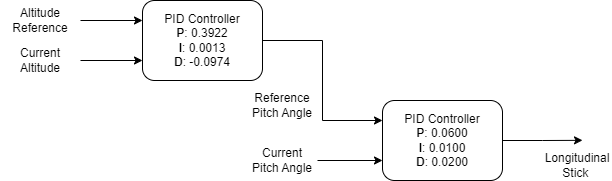
\includegraphics[width=0.75\linewidth]{Figures/longstickcontrol.drawio.png}
    \caption{Block diagram of longitudinal stick control through two closed-loop, PID controllers.}\label{fig:longstickcontrol}
\end{figure}

The throttle and propeller lever controllers use a PID and PI controller to correct their inputs (Table~\ref{tbl:throttleProp}). The throttle control is based on the commanded and current airspeed of the aircraft where the propeller lever is controlled based on maintaining at least \(93\% \) propeller efficiency. The airspeed for the throttle control is defined as the magnitude of the aircraft's velocity.

\begin{table}[!ht]
    \caption{Gains for the throttle and propeller lever closed-loop PID controllers.}\label{tbl:throttleProp}
    \centering
    \begin{tabular}{cccc}
        \toprule
        Controller      & Proportional & Integral  & Derivative \\
        \midrule
        Throttle Lever  & \(0.498\)    & \(0.098\) & \(-0.184\) \\
        Propeller Lever & \(0\)        & \(1\)     & \(0\)      \\
        \bottomrule
    \end{tabular}
\end{table}

The controllers provide inputs such that actuation of the control surfaces are deflected and can guide the aircraft in the desired direction at the desired speed while maintaining lower fuel consumption. With the implementation of the guidance system and control law, the full GNC loop is now complete. The following section describes the disturbances modeled on the aircraft so that controller inputs and outputs are different when running Monte-Carlo simulations for further analysis of the proposed navigation filter architecture.

\section{\textbf{Disturbance Modeling}}

As specified in Equation~\ref{eq:eulerIntegration}, the dynamics of the aircraft are disturbed by external forces that changes the behavior of the aircraft between simulations of the same trajectory. Ultimately, these changes lead to different control inputs and allow the Monte-Carlo analyses to emphasize the improvements of the proposed FVDM navigation filter.

For the study presented in this thesis, two disturbances are modeled {--} a wind model and uncertainties in the current altitude. The wind model is represented as a zero-mean white noise process from~\cite{khaghaniAutonomousVehicleDynamic2016}. Changes in the wind are important to simulation as wind greatly affect aircraft trajectories in reality. The modeling of wind as a white noise process provides a stochastic process that more closely resembles wind data collected from actual data collections~\cite{mwenegohaModelbasedTightlyCoupled2020}. In Chapter 2, it is clear that the pressure, temperature and density calculation stem from the ISA model; however, aircraft do not use this model on board. To simulate changes in these atmospheric parameters, measurements from a Pitot tube and temperature sensor are modeled as a zero-mean white noise process from~\cite{pieniazekDynamicResponsePitot2023}. Similar to the white-noise wind model, the measurements of pressure, temperature, and density must be variant enough to have different control inputs over the course of many Monte-Carlo simulations. The variance in these white noise models can be substituted for their respective variables in \(\mathbf{Q}_d\) (Equation~\ref{eq:Qd}).

\section{\textbf{Conclusions}}

The guidance systems and control laws provide the aircraft with meaningful control surface deflection that guide the aircraft to the desired destination. This chapter provided an overview about how the guidance system generates commanded control inputs from a user-defined trajectory created using Google Earth. Following the guidance system, the control law used in this thesis was covered with discussions about the PID control gains used for each of the four piloted control inputs during simulation. Finally, a discussion of the disturbances on the aircraft dynamics that influence different control inputs between simulations was described. The focus of this work is not on the guidance or controls of the flight vehicle presented in this thesis, for better detail of each the sections discussed during this chapter, the reader is asked to follow-up with the references cited above for more information.
\chapter{\textbf{Scenario Implementation and Results}}
% Introduction
This chapter presents results of two trajectories using the proposed navigation filter and its underlying components discussed in previous chapters. Each trajectory is subject to varying degrees of signal interference across multiple Monte-Carlo simulations. First, an overview of the Monte-Carlo analyses that will be presented for each trajectory is provided. Next, a discussion of the first trajectory and configuration file used for the simulations is presented. Following a description of trajectory one, Monte-Carlo analyses highlight the strong and weak points of the proposed navigation filter. Once the analyses of the first trajectory conclude, a description of trajectory two is presented, followed by a similar Monte-Carlo statistical analysis. Each Monte-Carlo case is composed of 100-run simulations for each trajectory subject to seven cases of signal degradation. To show the improved performance of the proposed navigation filter, a constant-velocity, kinematic model VDFLL~\cite{grierPositionNavigationTiming} is shown as a comparison. This standard VDFLL processes the same trajectories at the same cases of signal degradation.

\section{\textbf{Monte-Carlo Analyses}}
Originally named after a famous casino in Monaco, the Monte-Carlo analysis is a model to predict the probability of an outcome given the presence of random variables~\cite{mariettaMonteCarloError2013}. For the deeply-coupled FVDM, a number of random variables exists. For one, the true states of the aircraft are disturbed by wind, causing the aircraft to veer from the desired target line, that is, between simulations, the simulated aircraft will not fly the same flight path every time, regardless of having the same set of waypoints. For the purpose of this work, these wind disturbances are modeled with the same magnitude {--} interference and trajectory notwithstanding. Within the VT algorithms, the correlator simulator features noise that occurs at every measurement step, meaning no correlators (Equation~\ref{eq:correlators}) will be the same between simulations for the same time step. For the correlator simulation tool presented in this thesis, the random noise placed onto the correlators is a function of the interference level. As demonstrated by Equation~\ref{eq:CN0}, higher variance noise when compared to the amplitude of the cross-correlated local and received signal leads to an overall lower \(C/N_0\) ratio, which is demonstrated by the results later on in this chapter.

For each of the trajectories presented in this chapter, the 100-run Monte-Carlo simulations will evaluate the two different navigation filters for their probability to track the GPS signal given \(C/N_0\) degradation. Furthermore, Monte-Carlo analysis on code phase and carrier frequency error over a range of \(C/N_0\) values is presented. For the pose and attitude estimation results, the Monte-Carlo simulation will provide an average Latitude, Longitude and Altitude estimate compared to the true state of the receiver, along with velocity magnitudes (speed) for the same comparison. As will be discussed later, one of the benefits in using the proposed navigation solution is the ability to estimate angular rates and Euler attitude of the aircraft during simulation. The Monte-Carlo analysis will present the average error in comparison with the true angular rates and Euler attitude as well, but only for the deeply-coupled FVDM, as the standard VDFLL implementation does not have this capability. Lastly, the Monte-Carlo analysis of the 100-run simulations will compare the clock bias and clock drift estimates from both filters compared to the true clock bias and clock drift of the embedded OCXO on board.


\section{\textbf{First Trajectory}}
For the first trajectory, the aircraft is simulated for a straight flight path while maintaining a constant altitude of 500 meters above sea level (Figure~\ref{fig:trajectory1}).

\begin{figure}[!ht]
    \centering
    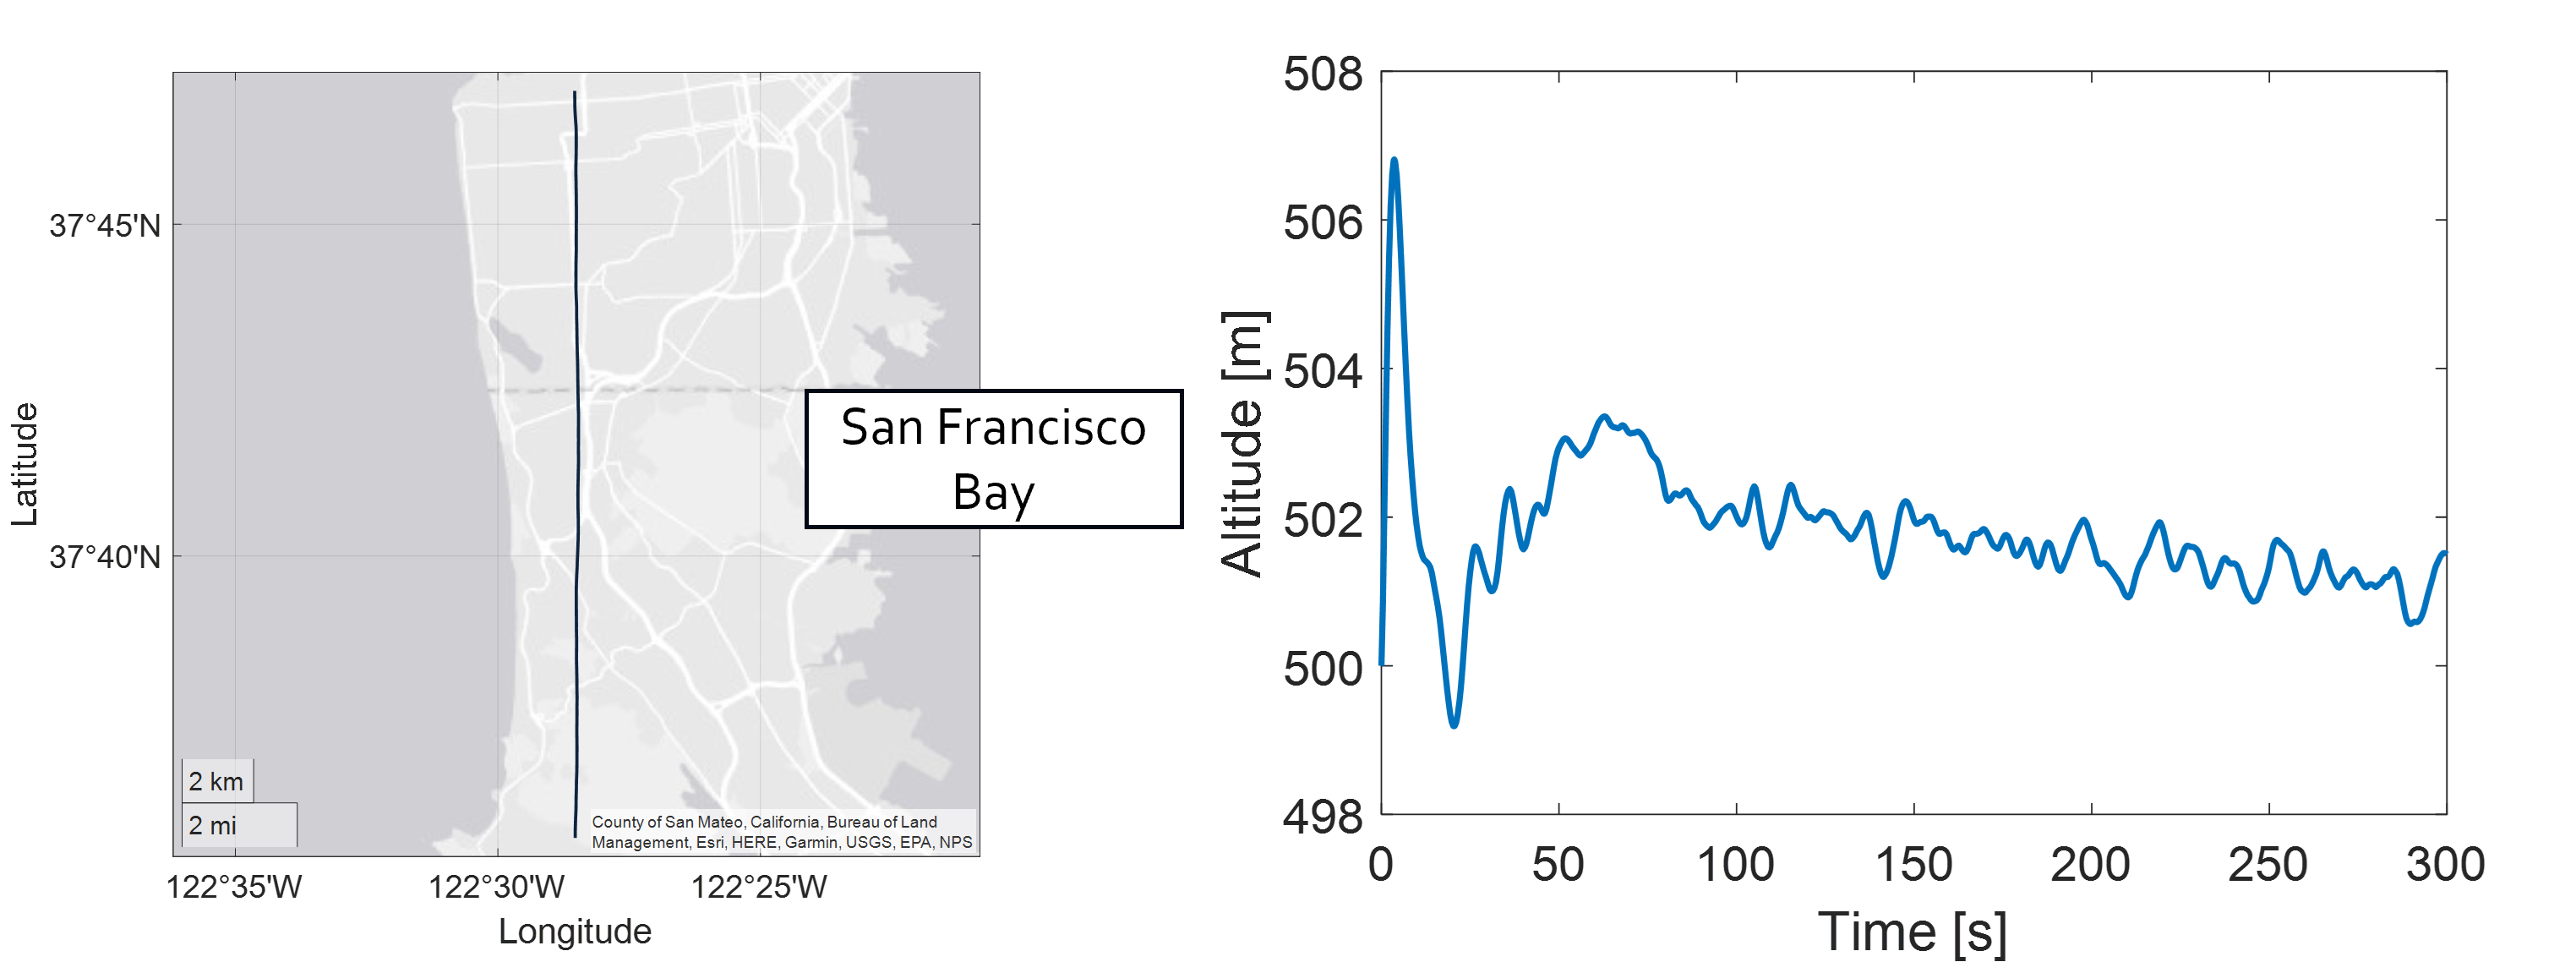
\includegraphics[width=0.9\linewidth]{Figures/Results/trajectory1.png}
    \caption{(Left) Top-view of simulated flight path for trajectory one. (Right) Altitude of flight path for trajectory one.}\label{fig:trajectory1}
\end{figure}

It is assumed that the initial position of the receiver is known when the simulation begins, avoiding the need to perform scalar tracking loops on the received signal data as discussed previously. For the first trajectory, the receiver aboard the aircraft is subject to seven different cases of interference that degrade the signals from the nine tracked channels (Table~\ref{tbl:interferenceCases}). The receiver is subject to these degraded power levels for the entirety of the 60 second simulations.

\begin{table}[!ht]
    \caption{Signal power for each case applied to each trajectory.}\label{tbl:interferenceCases}
    \centering
    \begin{tabular}{cc}
        \toprule
        Case & \(C/N_0\) [dB-Hz] \\
        \midrule
        1    & 45                \\
        2    & 35                \\
        3    & 25                \\
        4    & 22                \\
        5    & 20                \\
        6    & 18                \\
        7    & 16                \\
        8    & 15                \\
        9    & 10                \\
        10    & 5                \\
        11    & 2                \\
        \bottomrule
    \end{tabular}
\end{table}

From Table~\ref{tbl:trajectory}, several parameters are configurable to meet the desired simulation of the user.

\begin{table}[!ht]
    \caption{Initial conditions for simulated trajectory from Figure~\ref{fig:trajectory1}.}\label{tbl:trajectory}
    \centering
    \begin{tabular}{lcc}
        \toprule
        \textbf{Condition}       & \textbf{Value}                                      & \textbf{Units}                     \\
        \midrule
        Date                     & June 15, 2022                                       & \textit{DateTime} Object           \\
        Duration                 & 300                                                 & \(s\)                              \\
        Monte-Carlo Runs         & 100                                                 & {--}                               \\
        Frequency                & 200                                                 & Hz                                 \\
        Trajectory               & \textit{StraightFlightPath.mat}                     & See Chapter 5                      \\
        Velocity Disturbance     & \(\left[300, \; 300, \; 0\right]\)                  & \(m/s\)                            \\
        Angular Rate Disturbance & \(\left[10^{-12}, \; 10^{-12}, \; 10^{-12}\right]\) & \(rad/s\)                          \\
        Clock Type               & OCXO                                                & {--}                               \\
        Initial Velocity         & \(\left[75, \; 0, \; 0\right]\)                     & \(m/s\)                            \\
        Initial Angular Rate     & \(\left[0, \; 0, \; 0\right]\)                      & \(rad/s\)                          \\
        Initial Position         & \(\left[0.65617, \; -2.1376, \; 500\right]\)        & \(\left[rad, \; rad, \; m\right]\) \\
        Initial Attitude         & \(\left[0, \; 0, \; 0\right]\)                      & \(rad\)                            \\
        Initial Clock Terms      & \(\left[0, \; 0\right]\)                            & \(\left[m, \; m/s\right]\)         \\
        Channel \(C/N_0\)        & \(45,\,35,\,25,\,22,\,20,\,18,\,16,\,15,\,10,\,5,\,2\)                & dB-Hz                              \\

        \bottomrule
    \end{tabular}
\end{table}
Date is used to pull the specified Rinex file from~\cite{nollCrustalDynamicsData2010}. This Rinex file is then parsed for its ephemeris and used to propagate the GPS satellites during the simulation. Figure~\ref{fig:skyplot} shows the available satellites at the first time step for June 15, 2022 used in this work.

\begin{figure}[!ht]
    \centering
    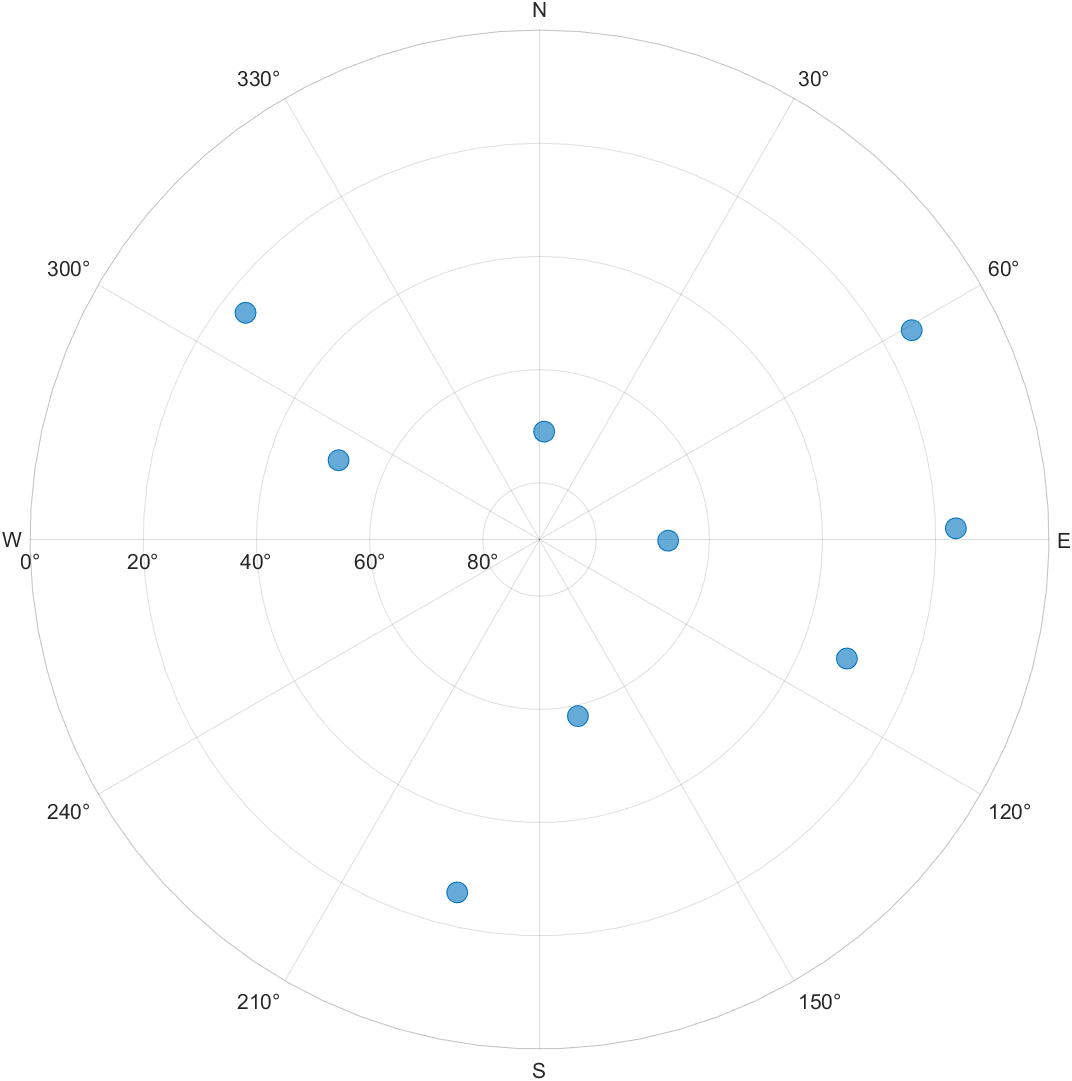
\includegraphics[width=0.8\linewidth]{Figures/Results/skyplot.png}
    \caption{Orange dots signify satellite locations at the start of the simulations given the date of broadcast ephemeris. Black dots signify satellites that are in-view but are discarded due to the 10 degree mask angle used. The green triangle represents the initial receiver position.}\label{fig:skyplot}
\end{figure}
Duration and Monte-Carlo Runs specify the length of each simulation in seconds and the number of simulations for each scenario and/or case. For the work presented in thesis, 100 simulation Monte-Carlo runs are used for analyses. Based on~\cite{khaghaniAssessmentVDMbasedAutonomous2018,khaghaniAutonomousVehicleDynamic2016,mwenegohaModelbasedTightlyCoupled2020} and time to completion for each simulation, 100 is enough to show the general trend for statistical purposes. The trajectory is specified as a -mat file. The creation of the trajectory is detailed in Chapter 5. Trajectory one is a baseline case where it is expected that both the deeply-coupled FVDM and constant-velocity kinematic model both perform well.  As explained in Chapter 5, disturbances are modeled onto the trajectory of the aircraft as the FVDM is not perfect. External conditions such as wind and various atmospheric effects alter the behavior of the Diamond DA-40 slightly. These disturbances are defined as Velocity and Angular Rate in Table~\ref{tbl:trajectory}. Clock Type is the embedded receiver clock modeled during the simulation. More information on the different types of clocks can be found in Chapter 4. For the purposes of this thesis, both trajectories and all cases of signal interference will use the OCXO as the embedded receiver oscillator. The initial states of the aircraft are defined by the given values. Since our trajectory specifies a mostly-north flight path, the north velocity component is specified to be 75 meters per second, while the other components are zero. Also, the pitch of the aircraft is specified as 4 degrees up, this is so the aircraft generates lift at the beginning of the simulations and does not enter a stall upon initialization. Lastly, the initial position of the aircraft is specified as the first waypoint location, for simplicity. The last configurable parameter is the initial channel \(C/N_0\) of the available satellites.


\subsection{\textbf{Monte-Carlo Analyses}}
From the Monte-Carlo results, several parameters can be analyzed for the performance improvements of the proposed navigation filter over the standard VDFLL kinematic model. This section begins with a comparison of the tracking-level results of the two filters subject to different levels of signal degradation.

For the range of signal interference presented in Table~\ref{tbl:interferenceCases}, the Root Mean Square Errors (RMSE) of both the code phase and carrier frequency shows the improved performance by using the deeply-coupled FVDM in GPS-challenged environments (Figure~\ref{fig:codecarrierstraight}). During simulations where the signal was slightly degraded or benign (i.e.\ channel power greater than \(35\) dB-Hz) the standard velocity implementation of the VDFLL actually performs better on average than the proposed navigation filter. This is most likely due to the FVDM becoming over confident during simulation. This is more evident from Tables~\ref{tbl:straight35FVDM} and~\ref{tbl:straight35CV} where the position RMSE, STandard Deviation (STD), and maximum error from the constant velocity kinematic model are marginally better.

\begin{figure}[!ht]
    \begin{subfigure}{.45\textwidth}
        \centering
        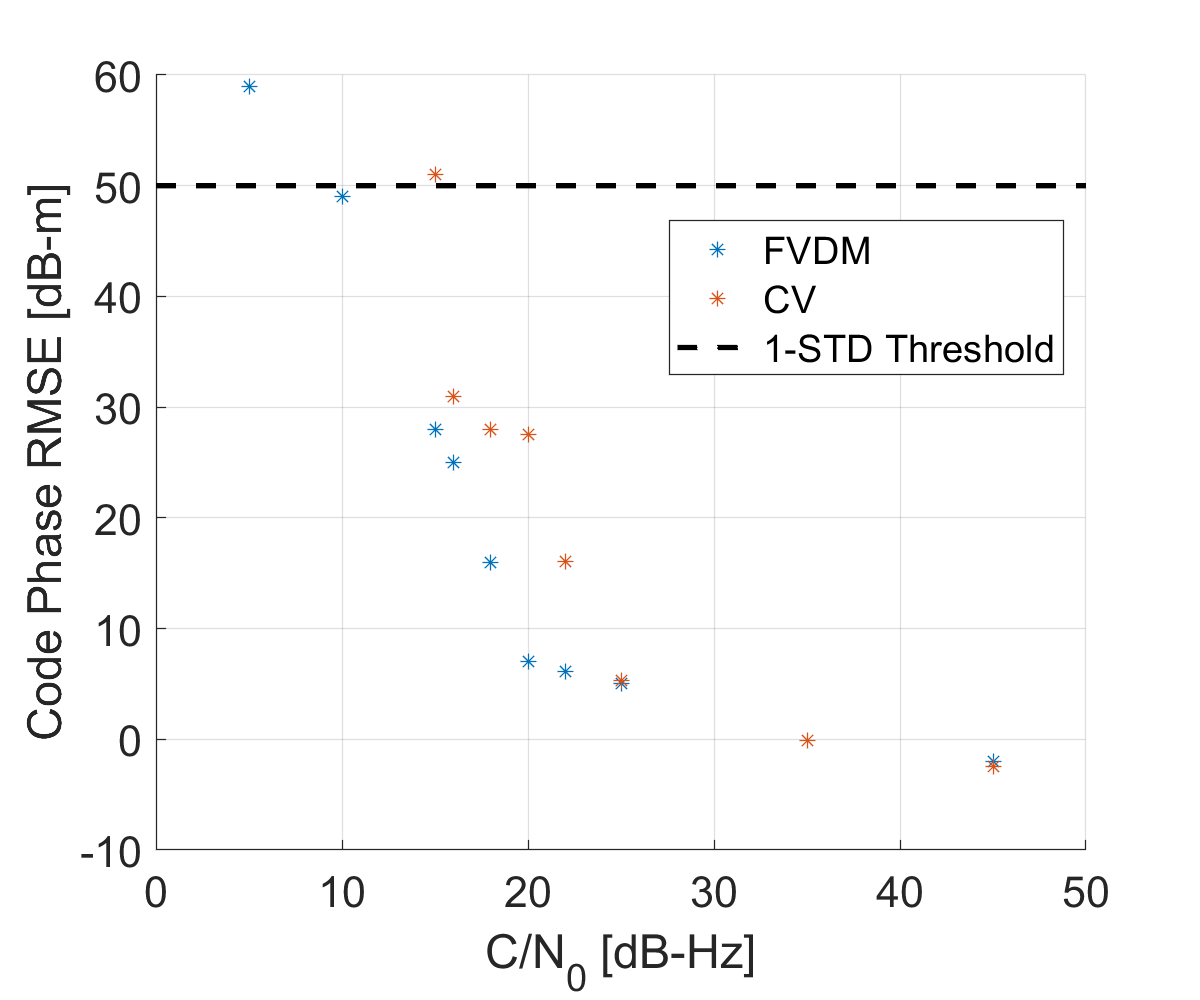
\includegraphics[width=1\linewidth]{Figures/straight/codephaseRMSEstraight.png}
    \end{subfigure}%
    \begin{subfigure}{.45\textwidth}
        \centering
        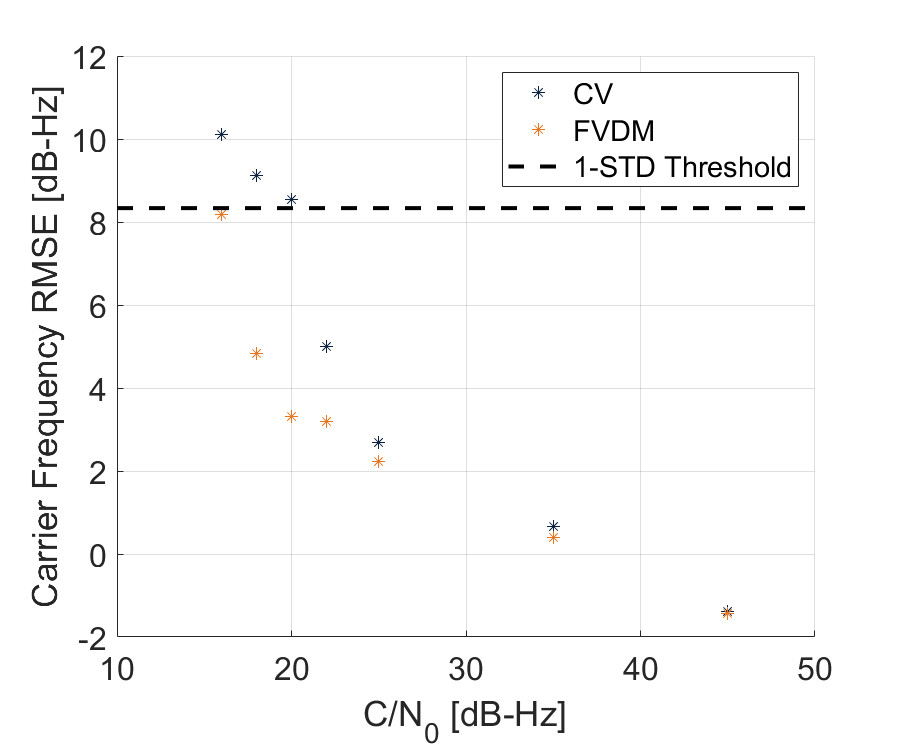
\includegraphics[width=1\linewidth]{Figures/straight/carrFreqRMSEstraight.png}
    \end{subfigure}
    \caption{Code phase and carrier frequency RMSE as a function of signal power, specified in dB-Hz.}\label{fig:codecarrierstraight}
\end{figure}

\begin{table}[!ht]
    \caption{RMSE, STD, and maximum error from 100-run Monte Carlo simulation when the deeply-coupled FVDM is subject to a degraded signal power level of \(35\) dB-Hz.}\label{tbl:straight35FVDM}
    \centering
    \begin{tabular}{ccccc}
        \toprule
                  & Position [m] & Speed [m/s] & Clock Bias [m] & Clock Drift [m/s] \\
        \midrule
        RMSE      & 0.23443      & 0.066059    & 0.013062       & 0.002834          \\
        STD       & 0.11305      & 0.030674    & 0.17509        & 0.0032795         \\
        Max Error & 0.72197      & 0.22588     & 0.05835        & 0.009             \\
        \bottomrule
    \end{tabular}
\end{table}

\begin{table}[!ht]
    \caption{RMSE, STD, and maximum error from 100-run Monte Carlo simulation when the standard VT receiver is subject to a degraded signal power level of \(35\) dB-Hz.}\label{tbl:straight35CV}
    \centering
    \begin{tabular}{ccccc}
        \toprule
                  & Position [m] & Speed [m/s] & Clock Bias [m] & Clock Drift [m/s] \\
        \midrule
        RMSE      & 0.093008     & 0.087402    & 0.013897       & 0.0032735         \\
        STD       & 0.048771     & 0.038728    & 0.015186       & 0.0040279         \\
        Max Error & 0.25751      & 0.26045     & 0.033083       & 0.009487          \\
        \bottomrule
    \end{tabular}
\end{table}

However, when the signal power is less than \(35\) dB-Hz, the deeply-coupled FVDM presents steady performance improvements as the interference grows stronger. For carrier frequency error, the deeply-coupled filter breaks down at roughly \(16\) dB-Hz, where the theoretical \(8.33\) dB-Hz STD from~\cite{lashleyPerformanceAnalysisVector2009} is met. For the standard VDFLL implementation, this criteria is met at roughly \(20\) dB-Hz. The probability that the vector tracking loops are able to maintain channel lock for an entire simulation is shown in Figure~\ref{fig:trackingprobability1}.

\begin{figure}[!ht]
    \centering
    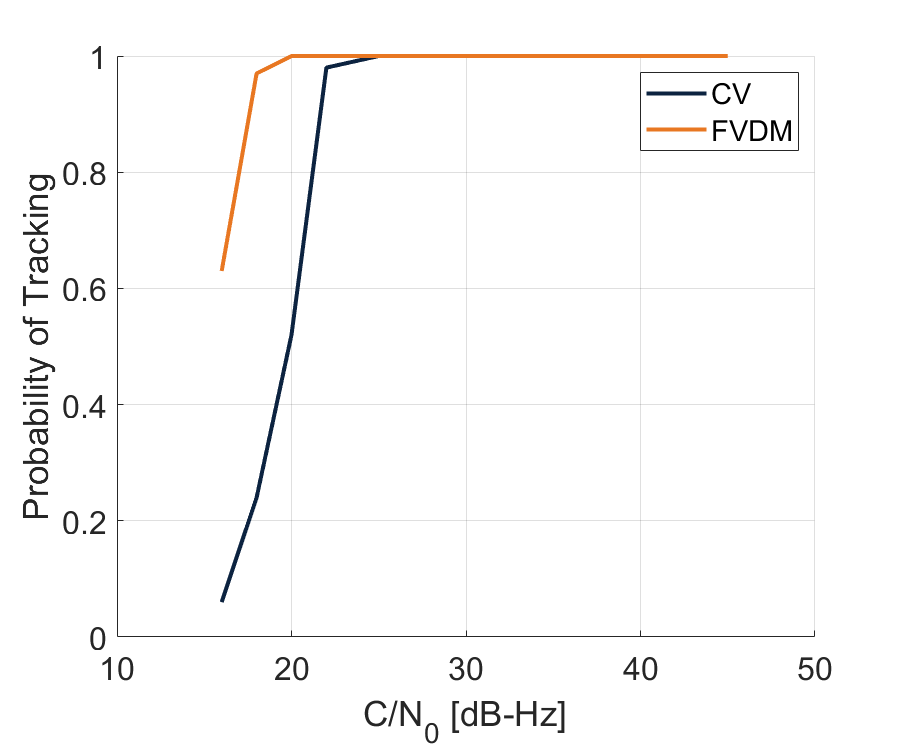
\includegraphics[width=0.5\linewidth]{Figures/straight/trackingprobstraight.png}
    \caption{The probability that each navigation filter is able to maintain channel lock throughout the simulation across different levels of signal interference.}\label{fig:trackingprobability1}
\end{figure}

Based on Figure~\ref{fig:trackingprobability1}, the proposed navigation filter shows approximately \(100\% \) tracking probability \(5\) dB-Hz greater than the standard constant-velocity kinematic model. As stated previously, one of the benefits in utilizing the FVDM within a sensor fusion framework is the acknowledgment of aircraft behavior given a set of control inputs. This allows the presented filter to rely less on the degraded correlator measurements from GPS\@. The pose estimates from the navigation filter reflect the performance of the vector tracking loops to maintain lock under different levels of signal degradation (Figure~\ref{fig:GEOPLOT1}).

\begin{figure}[!ht]
    \begin{subfigure}{.45\textwidth}
        \centering
        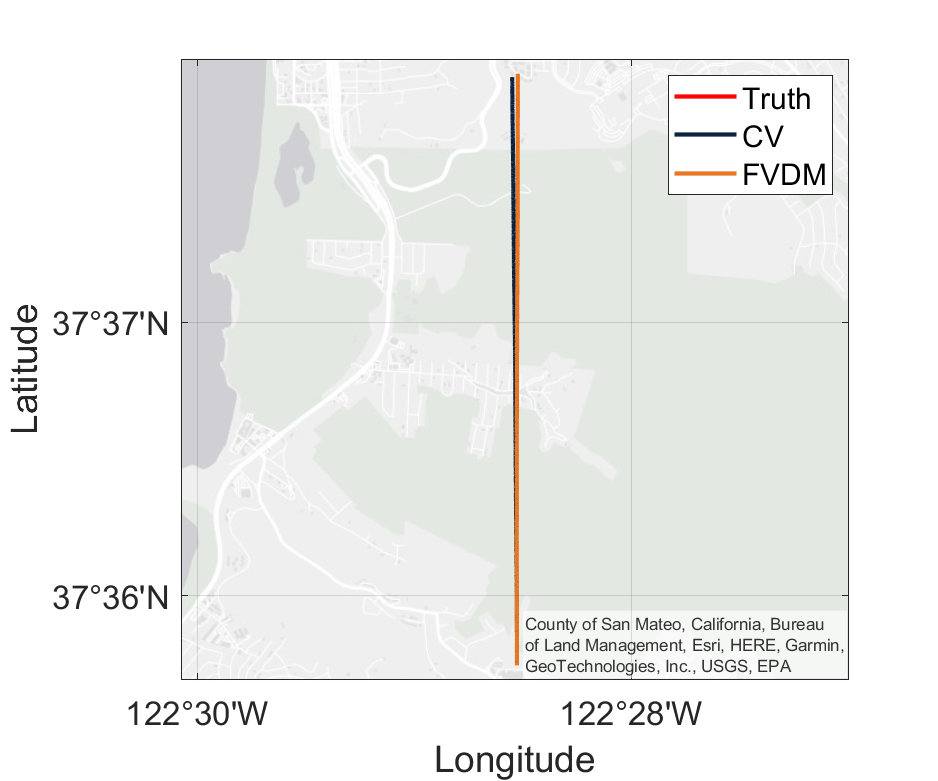
\includegraphics[width=1\linewidth]{Figures/straight/20/GEOPLOT.png}
    \end{subfigure}%
    \begin{subfigure}{.45\textwidth}
        \centering
        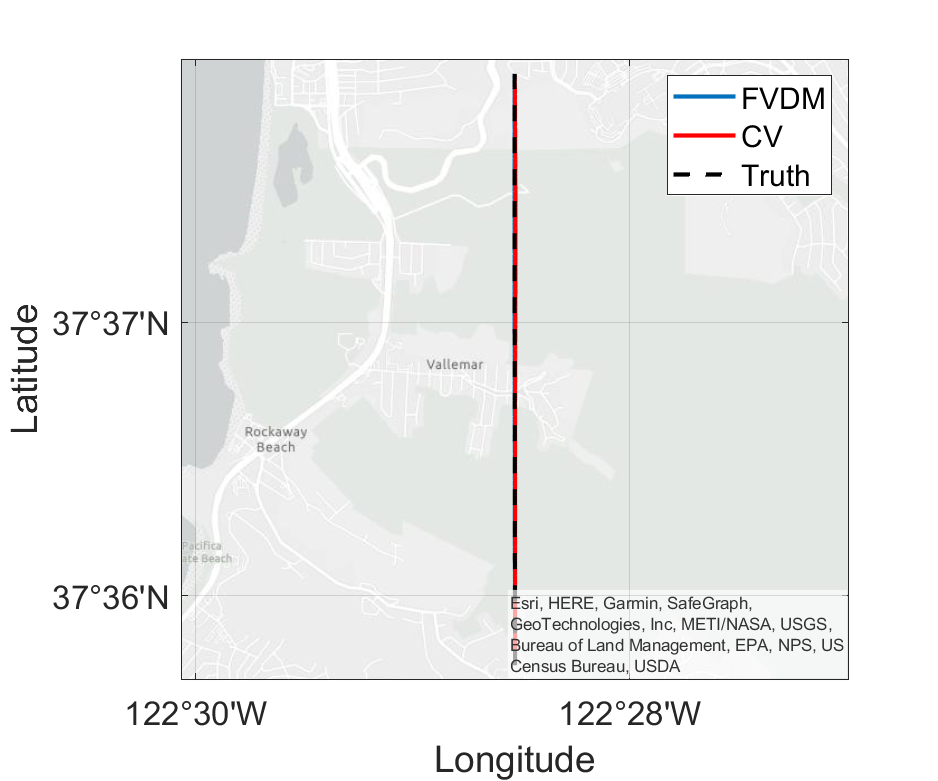
\includegraphics[width=1\linewidth]{Figures/straight/25/GEOPLOT.png}
    \end{subfigure}
    \caption{Average Latitude and Longitude of the FVDM and standard VDFLL implementation compared to the truth trajectory. The left figure is when both simulations had a signal power of \(20\) dB-Hz. The right figure is with a signal power of \(25\) dB-Hz.}\label{fig:GEOPLOT1}
\end{figure}

Even with the straight, baseline trajectory, the standard constant velocity filter begins to drift slightly when the GPS measurements are unreliable. This is partially due to the non-linear velocity at the beginning of the simulation. However, even though this is the case, the proposed navigation filter has no problem maintaining accurate tracking estimates. Based on Figure~\ref{fig:codecarrierstraight}, the deeply integrated FVDM maintains great position estimates with each channel's signal power down to \(16\) dB-Hz (Figure~\ref{fig:GEOPLOT2}). For the position estimates from the standard VDFLL implementation, the greatest error is shown in the downward direction (Figure~\ref{fig:Altitude1}).

\begin{figure}[!ht]
    \centering
    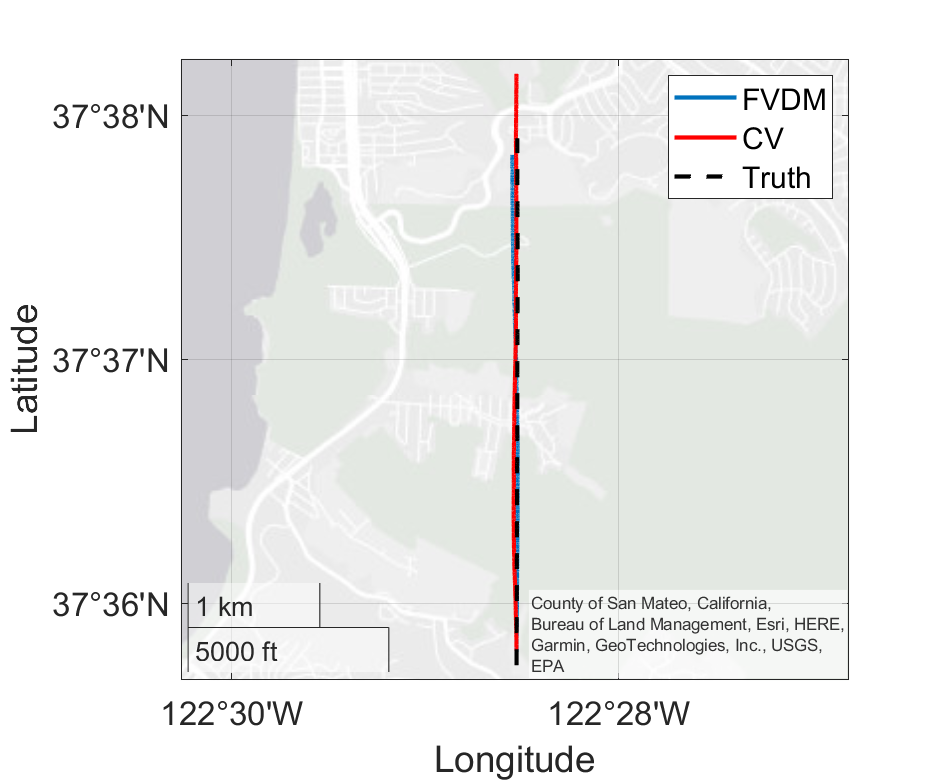
\includegraphics[width=0.5\linewidth]{Figures/straight/15/GEOPLOT.png}
    \caption{Average Latitude and Longitude of the FVDM and standard VDFLL implementation compared to the truth trajectory when subject to a degraded signal power of \(16\) dB-Hz.}\label{fig:GEOPLOT2}
\end{figure}



\begin{figure}[!ht]
    \begin{subfigure}{.45\textwidth}
        \centering
        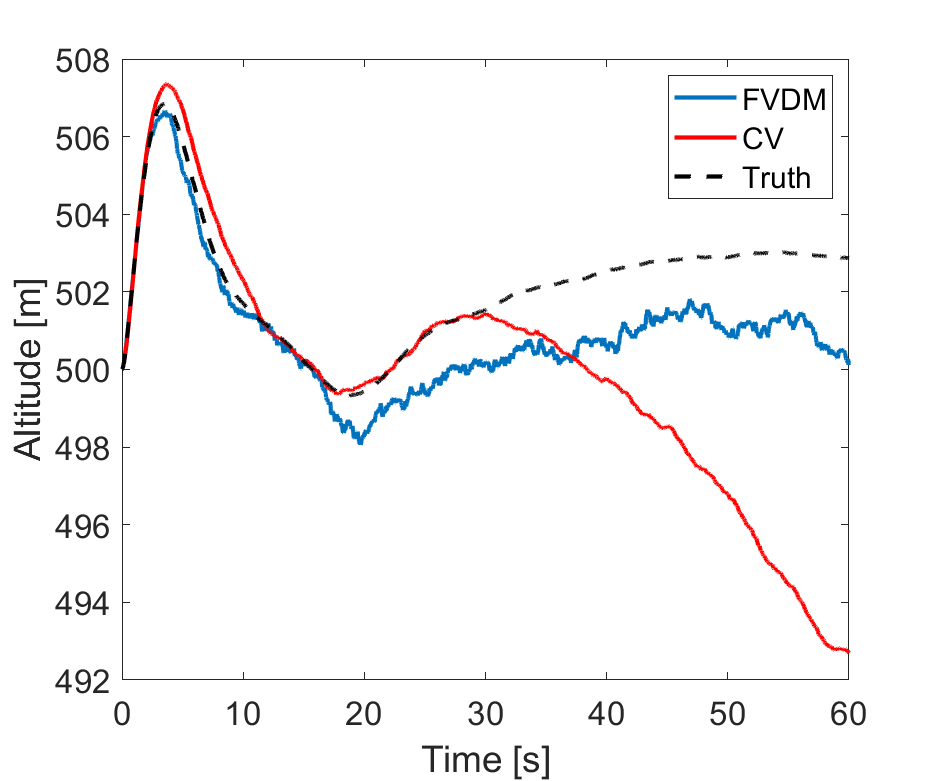
\includegraphics[width=1\linewidth]{Figures/straight/20/ALTITUDE.png}
    \end{subfigure}
    \begin{subfigure}{.45\textwidth}
        \centering
        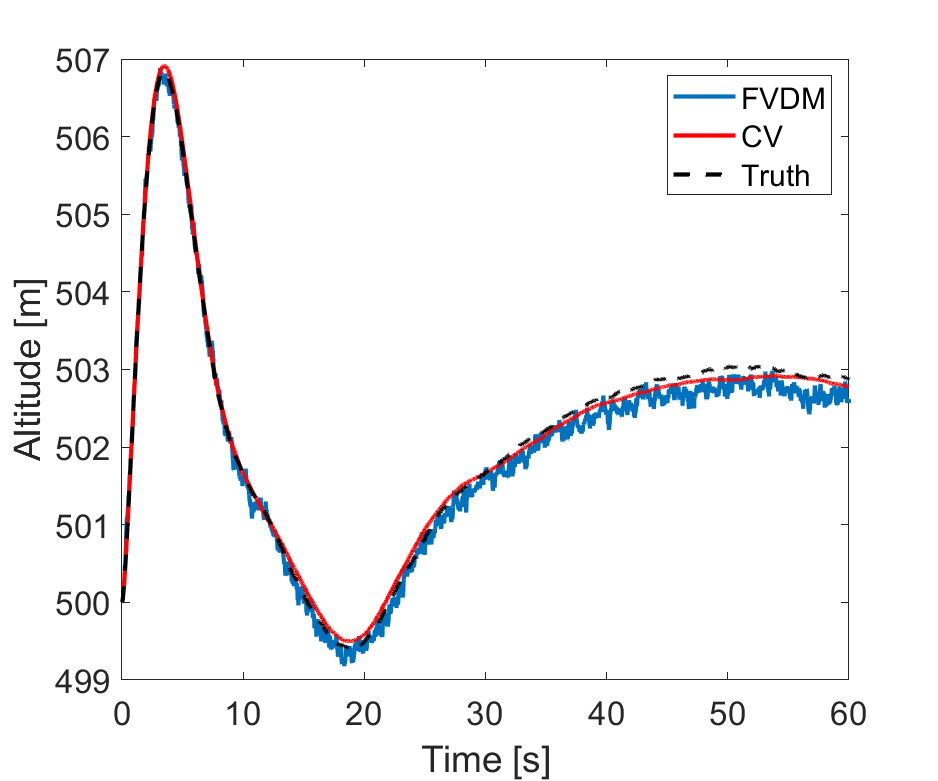
\includegraphics[width=1\linewidth]{Figures/straight/25/ALTITUDE.png}
    \end{subfigure}
    \caption{Average altitude estimates of the FVDM and standard VDFLL implementation compared to the truth trajectory. The left figure is when both simulations had a signal power of \(20\) dB-Hz. The right figure is with a signal power of \(25\) dB-Hz.}\label{fig:Altitude1}
\end{figure}

This is simply due to the lack of geometric diversity between the satellites sending the measurements. One way to solve this problem would be to include LEO satellites or signals of opportunity for improved altitude estimates from more diverse measurements. The poor assumption that the acceleration of the aircraft is zero-mean can be seen by the speed estimates in the constant-velocity kinematic model (Figure~\ref{fig:Speed1})

\begin{figure}[!ht]
    \begin{subfigure}{.45\textwidth}
        \centering
        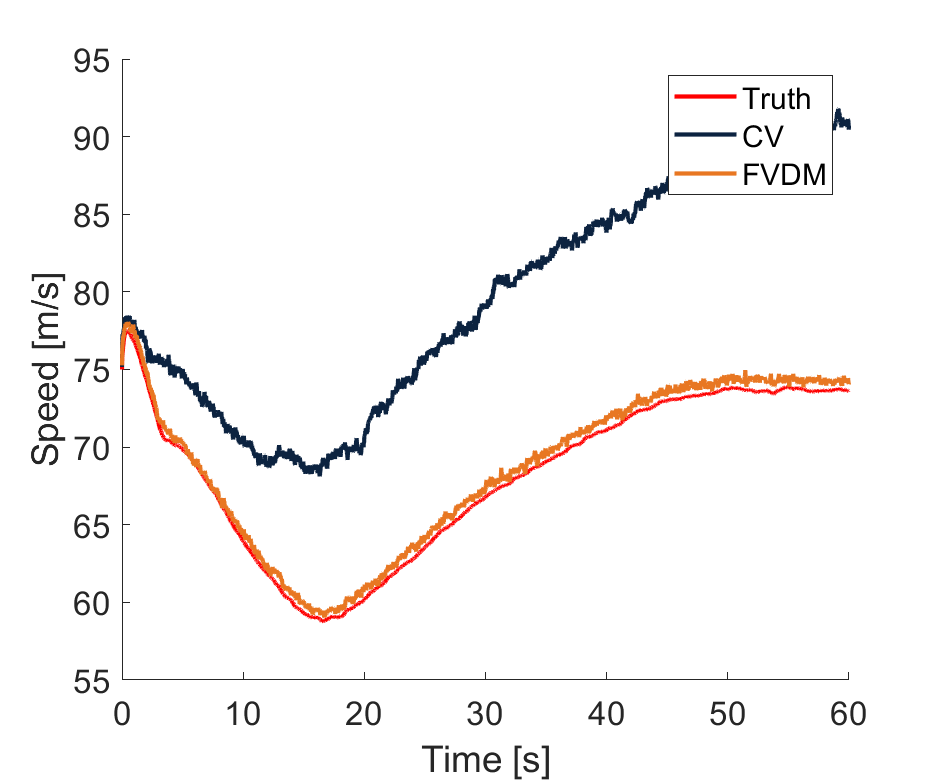
\includegraphics[width=1\linewidth]{Figures/straight/20/SPEED.png}
    \end{subfigure}
    \begin{subfigure}{.45\textwidth}
        \centering
        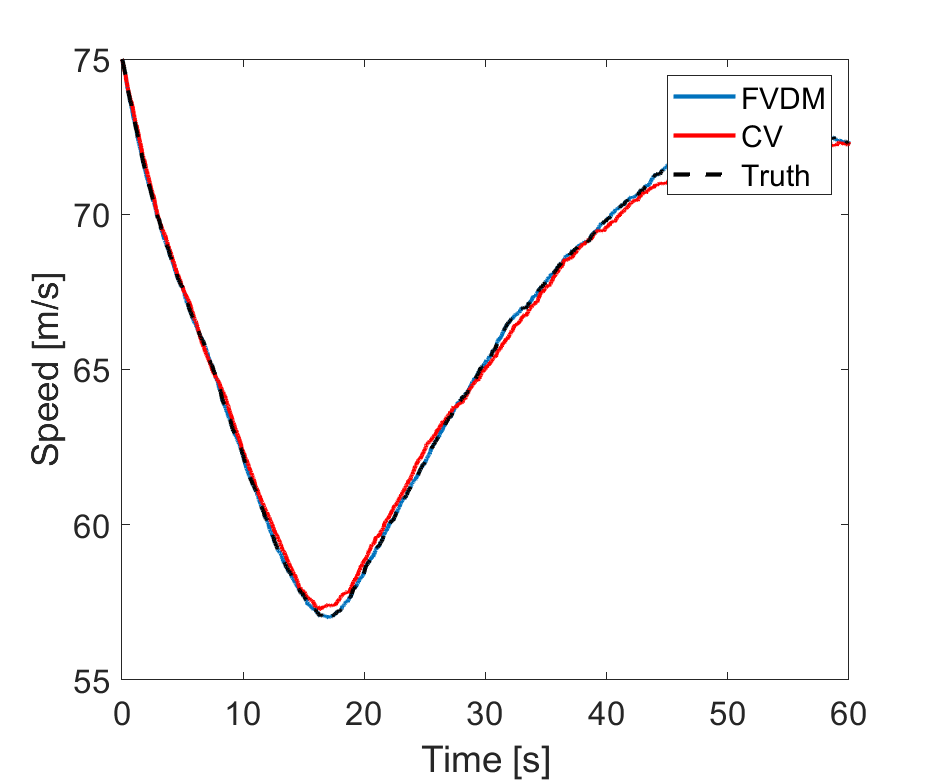
\includegraphics[width=1\linewidth]{Figures/straight/25/SPEED.png}
    \end{subfigure}
    \caption{Average speed estimates of the FVDM and standard VDFLL implementation compared to the truth trajectory. The left figure is when both simulations had a signal power of \(20\) dB-Hz. The right figure is with a signal power of \(25\) dB-Hz.}\label{fig:Speed1}
\end{figure}

When the correlator measurements from the receiver become unreliable, the constant velocity filter has no choice but to rely on its own prediction of aircraft velocity. On the fundamental basis that the velocity is the integral of a zero-mean acceleration, it leads the standard implementation to a heavily biased velocity prediction, thus deviating from the true states. Apart from the position and velocities, both filters also estimate the bias and drift of the embedded clock. As stated before, the clock used during the simulations is an OCXO\@. Figure~\ref{fig:Clocks1} presents the average clock bias estimates for each filter at both \(20\) and \(25\) dB-Hz signal power, while Figure~\ref{fig:Clocks2} presents the average clock drift estimates from each filter for the same interference cases.

\begin{figure}[!ht]
    \begin{subfigure}{.45\textwidth}
        \centering
        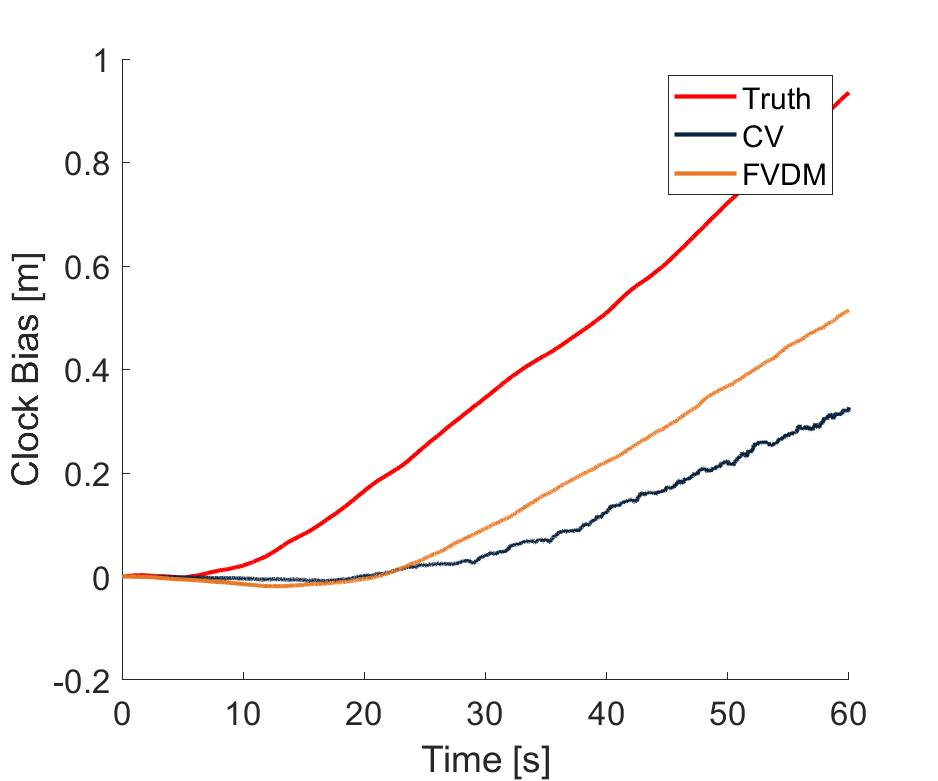
\includegraphics[width=1\linewidth]{Figures/straight/25/CLOCKBIAS.png}\
    \end{subfigure}
    \begin{subfigure}{.45\textwidth}
        \centering
        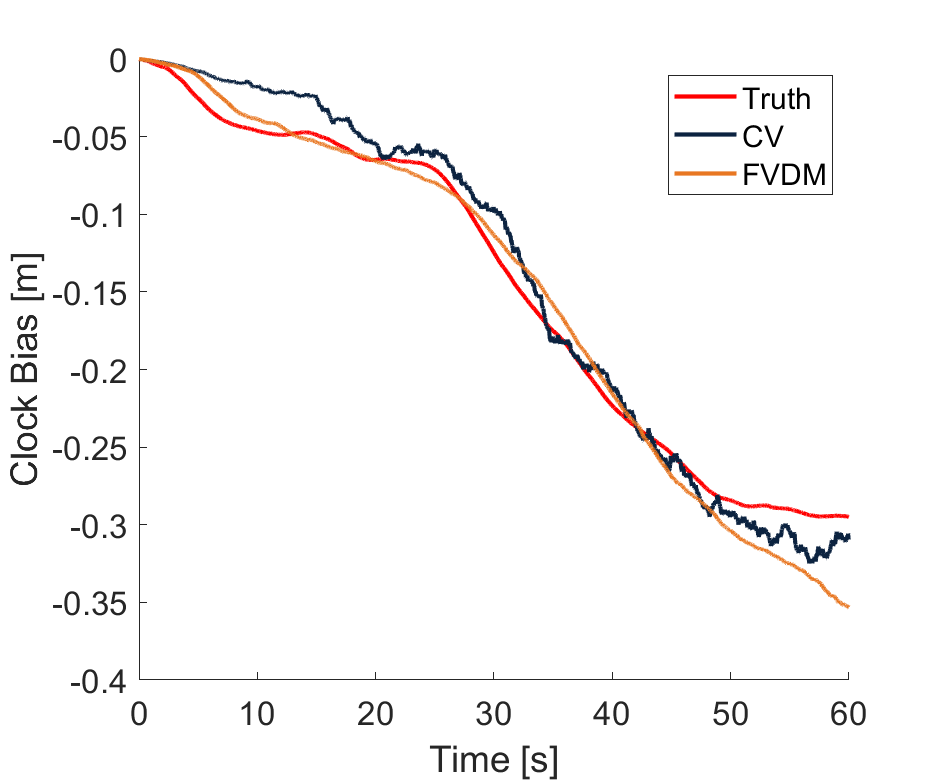
\includegraphics[width=1\linewidth]{Figures/straight/35/CLOCKBIAS.png}
    \end{subfigure}
    \caption{Average clock bias estimates of the FVDM and standard VDFLL implementation compared to the truth trajectory. The left figure is when both simulations had a signal power of \(20\) dB-Hz. The right figure is with a signal power of \(25\) dB-Hz.}\label{fig:Clocks1}
\end{figure}

\begin{figure}[!ht]
    \begin{subfigure}{.45\textwidth}
        \centering
        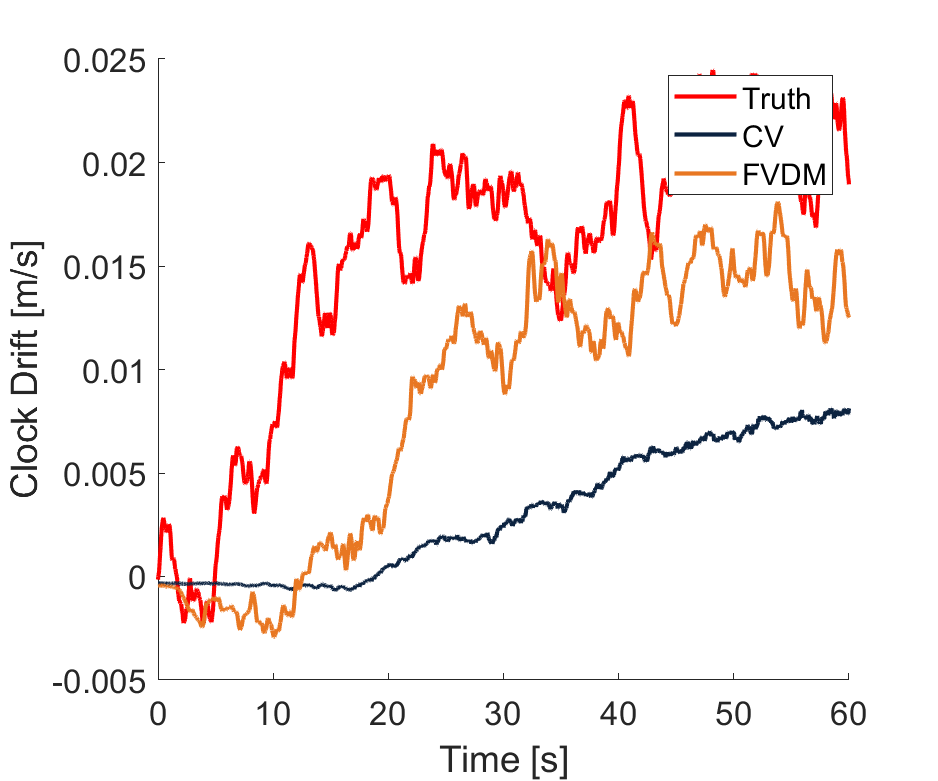
\includegraphics[width=1\linewidth]{Figures/straight/25/CLOCKDRIFT.png}\
    \end{subfigure}
    \begin{subfigure}{.45\textwidth}
        \centering
        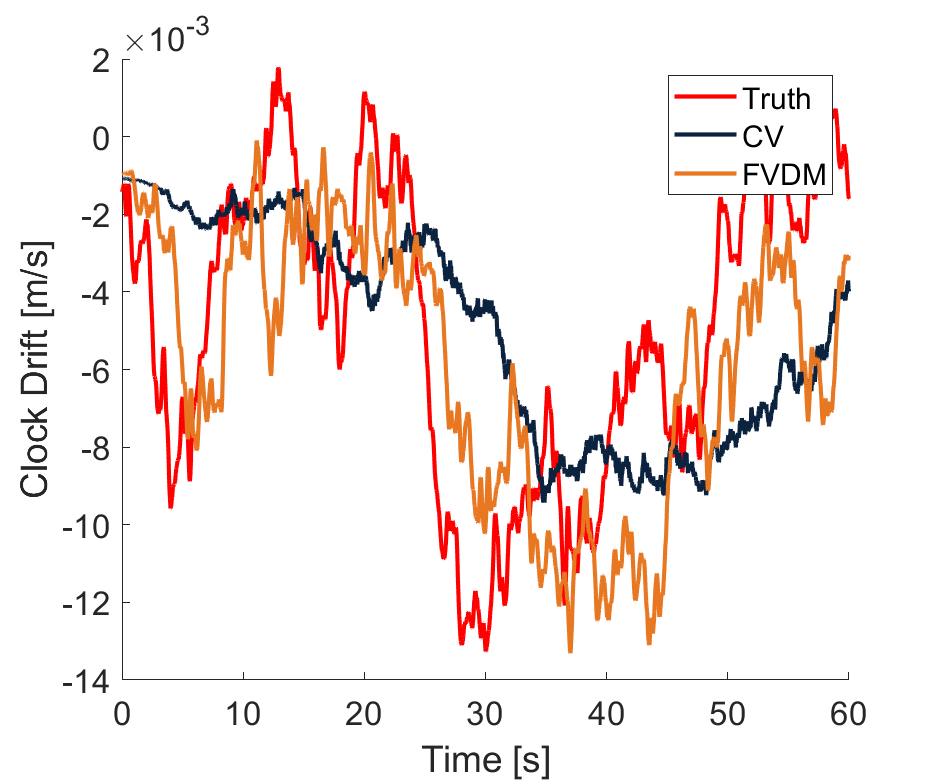
\includegraphics[width=1\linewidth]{Figures/straight/35/CLOCKDRIFT.png}
    \end{subfigure}
    \caption{Average clock drift estimates of the FVDM and standard VDFLL implementation compared to the truth trajectory. The left figure is when both simulations had a signal power of \(20\) dB-Hz. The right figure is with a signal power of \(25\) dB-Hz.}\label{fig:Clocks2}
\end{figure}

The clock model utilized from~\cite{wangKalmanFilterBasedIntegrity} is the same used on both filters, so similar performance should be expected. However, the deeply-coupled navigation filter still out performs the constant-velocity EKF in both cases. The errors in clock bias and clock drift are directly linked to position and velocity estimates seen before (Figures~\ref{fig:GEOPLOT1} and~\ref{fig:Speed1}). That is, the less error on the positional estimates means less likelihood of more error on the clock bias estimates. The same can be said for the velocity and clock drift estimates between the two filters.

As mentioned previously, the first trajectory was a baseline, litmus test where it is expected that both the proposed navigation filter and the constant velocity kinematic model would perform similarly. Regardless of the objective for the trajectory, in cases where the signal interference left the signal power to be less than \(25\) dB-Hz, the deeply-coupled FVDM begins to show improved performance. This is further illustrated by Tables~\ref{tbl:straight20FVDM} and~\ref{tbl:straight20CV} where the RMSE, STD, and maximum error found from the 100-run Monte Carlo analysis are shown for a subjected signal power of \(20\) dB-Hz.

\begin{table}[!ht]
    \caption{RMSE, STD, and maximum error from 100-run Monte Carlo simulation when the receiver is subject to a degraded signal power level of \(20\) dB-Hz.}\label{tbl:straight20FVDM}
    \centering
    \begin{tabular}{ccccc}
        \toprule
                  & Position [m] & Speed [m/s] & Clock Bias [m] & Clock Drift [m/s] \\
        \midrule
        RMSE      & 0.83733      & 0.27649     & 0.14072        & 0.0087105         \\
        STD       & 0.32434      & 0.13394     & 0.13147        & 0.0072989         \\
        Max Error & 1.8783       & 0.90375     & 0.48541        & 0.024451          \\
        \bottomrule
    \end{tabular}
\end{table}

\begin{table}[!ht]
    \caption{RMSE, STD, and maximum error from 100-run Monte Carlo simulation when the receiver is subject to a degraded signal power level of \(20\) dB-Hz.}\label{tbl:straight20CV}
    \centering
    \begin{tabular}{ccccc}
        \toprule
                  & Position [m] & Speed [m/s] & Clock Bias [m] & Clock Drift [m/s] \\
        \midrule
        RMSE      & 24.567       & 0.88208     & 0.17748        & 0.0088036         \\
        STD       & 10.287       & 0.34973     & 0.14068        & 0.005286          \\
        Max Error & 36.193       & 2.0585      & 0.50134        & 0.022316          \\
        \bottomrule
    \end{tabular}
\end{table}

\section{\textbf{Second Trajectory}}
For the second trajectory, the aircraft is simulated for a more dynamic flight pattern while commanded to climb to an altitude of 1150 meters above sea level (Figure~\ref{fig:trajectory2}). The dynamics induced by trajectory two show the effectiveness of the deeply-coupled FVDM to predict the behavior of the aircraft due to the additional angular rates and Euler attitude being estimated. It is assumed that the receiver knows it position beforehand when the simulation begins. Similarly to the first trajectory, the receiver aboard the aircraft is subject to seven different cases of interference that degrade the signals from the nine tracked channels (Table~\ref{tbl:interferenceCases}). The receiver is subject to these degraded power levels for the entirety of the 60 second simulation.

\begin{figure}[!ht]
    \centering
    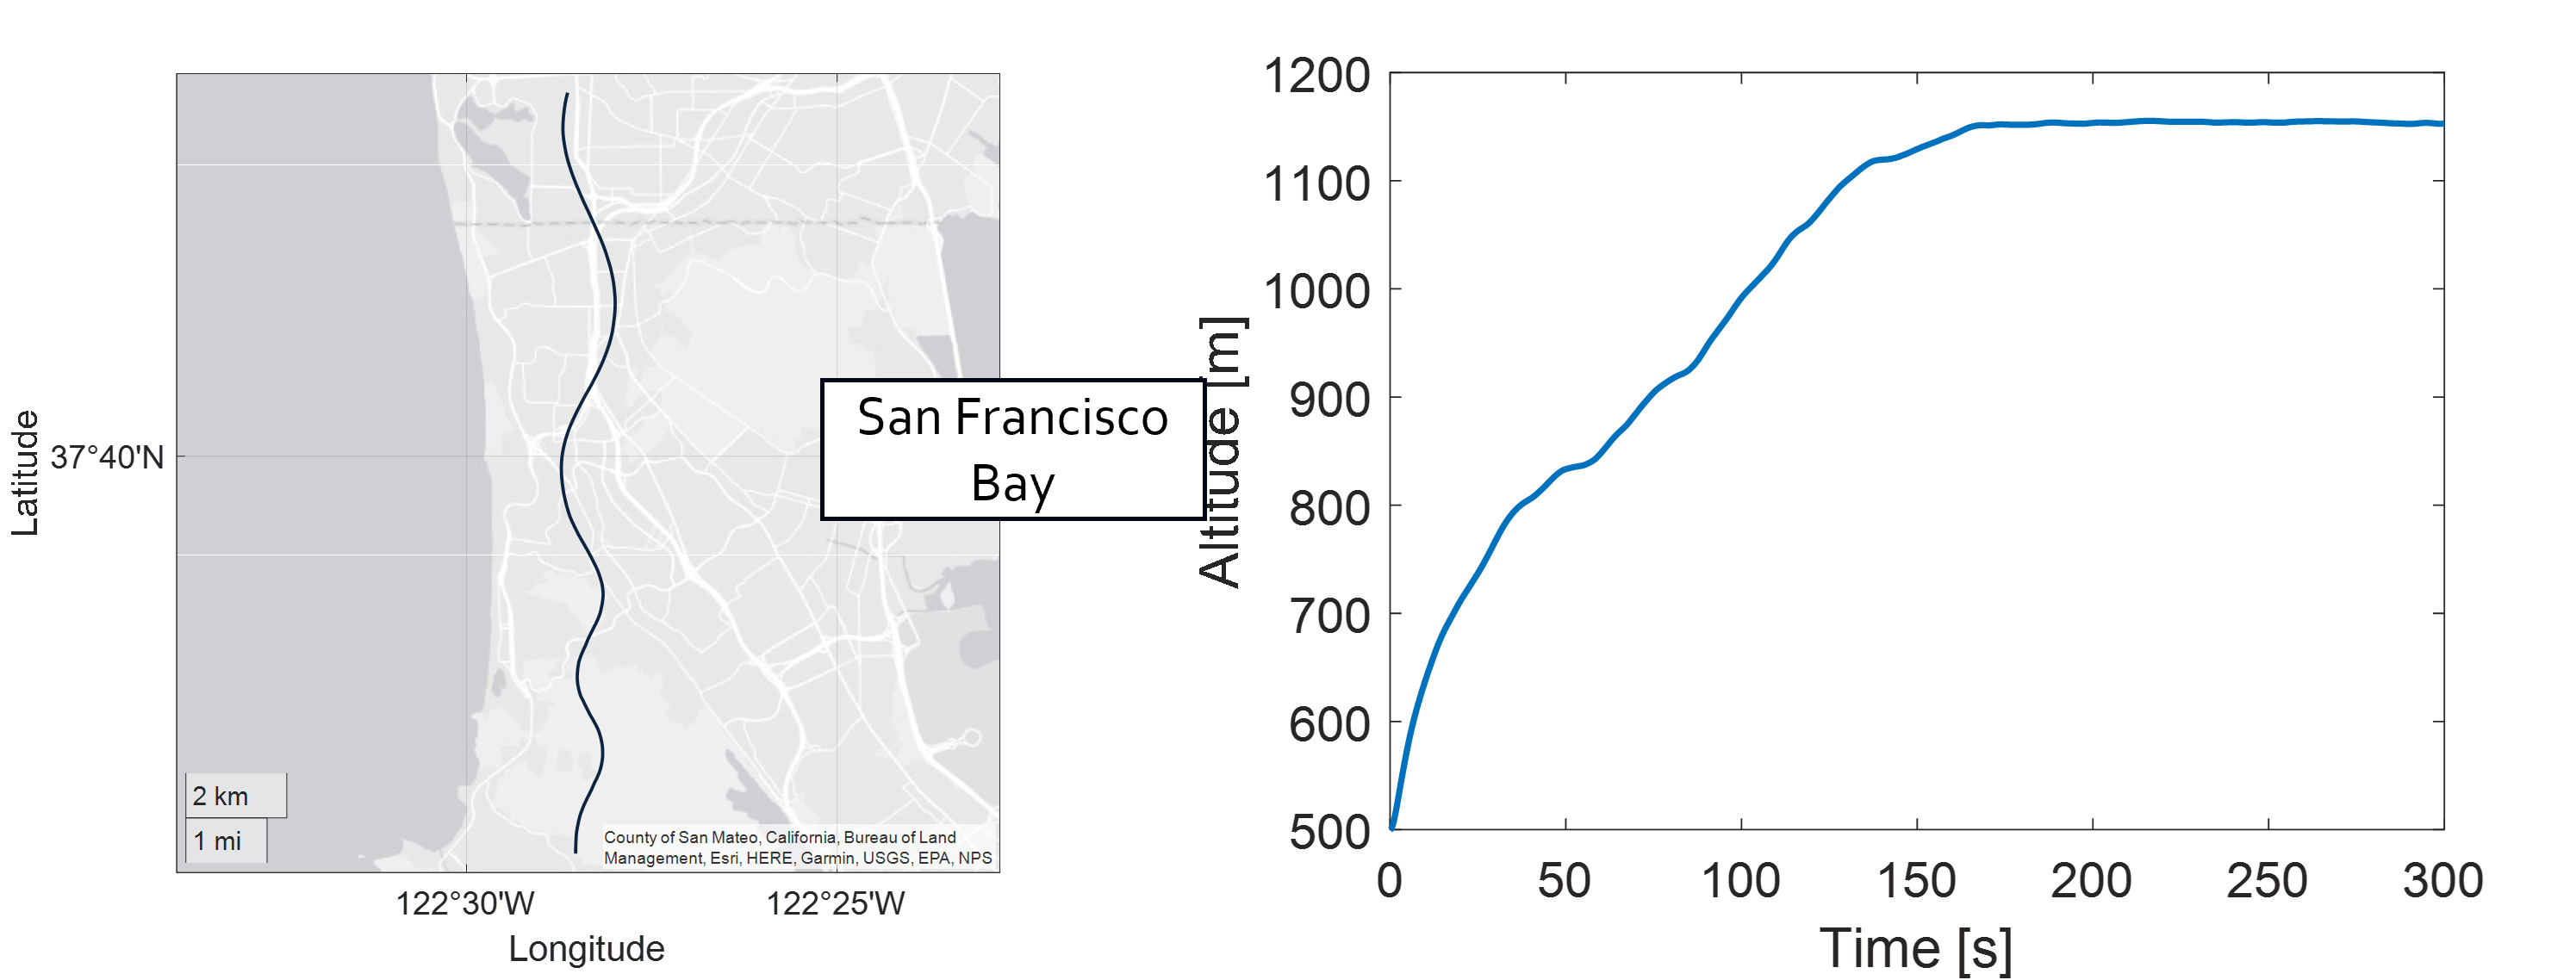
\includegraphics[width=\linewidth]{Figures/Results/trajectory2.png}
    \caption{(Left) Top-view of simulated flight path for the second trajectory. (Right) Altitude of second flight path where aircraft is commanded to climb to 1150 meters and then maintain the altitude for the remainder of the simulation.}\label{fig:trajectory2}
\end{figure}

It should be noted that the same cases of interference from the first trajectory still apply to trajectory two (Table~\ref{tbl:interferenceCases}). Furthermore, the only change in configuration between the first and second trajectory is the specified flight path. For this dynamic trajectory, \textit{SCurveFlightPath.mat} will be used in place of the \textit{StraightFlightPath.mat} used previously. The satellites found in-view utilizing the broadcast ephemeris file for the specified date are the same satellites used during the following simulations (Figure~\ref{fig:skyplot}). One of the benefits (on top of improved estimate performance) of utilizing the deeply-coupled FVDM is the capability to estimate the attitude and attitude rate of the aircraft during flight. This can be imperative for acrobatic or urban air mobility aircraft that roll, pitch, and yaw as their nominal flight motion. Similar to IMU and other hardware sensors, the excitation caused by the rolling and pitching motion of aircraft for trajectory two is expected to increase the performance of the position and velocity estimates along with the capability to maintain channel lock at heavier signal degradation.

\subsection{\textbf{Monte-Carlo Analyses}}
From Monte-Carlo results, several parameters can analyzed for the performance improvements of the proposed navigation filter over the standard VDFLL kinematic model. This section begins with an analysis of the signal-level results between the two filters and follows with an analysis of the state estimate performance for a range of \(C/N_0\) values. For the range of signal interference presented in table~\ref{tbl:interferenceCases}, the RMSE of both the code phase and carrier frequency shows improved performance by using the deeply-coupled FVDM in GPS-challenged environments (Figure~\ref{fig:codecarrierdyn}).

\begin{figure}[!ht]
    \begin{subfigure}{.45\textwidth}
        \centering
        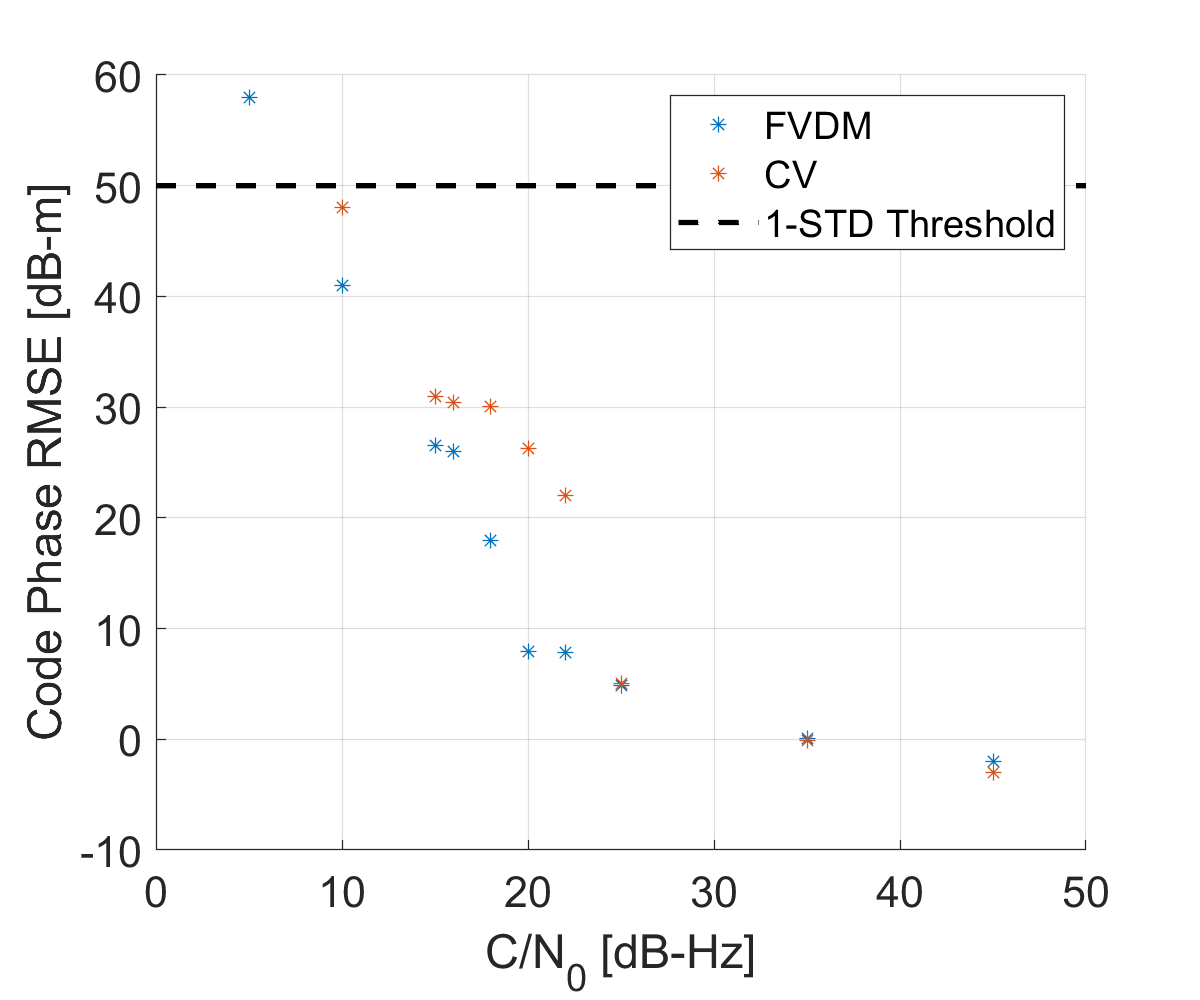
\includegraphics[width=1\linewidth]{Figures/dynamic/codephaseRMSEdyn.png}
    \end{subfigure}%
    \begin{subfigure}{.45\textwidth}
        \centering
        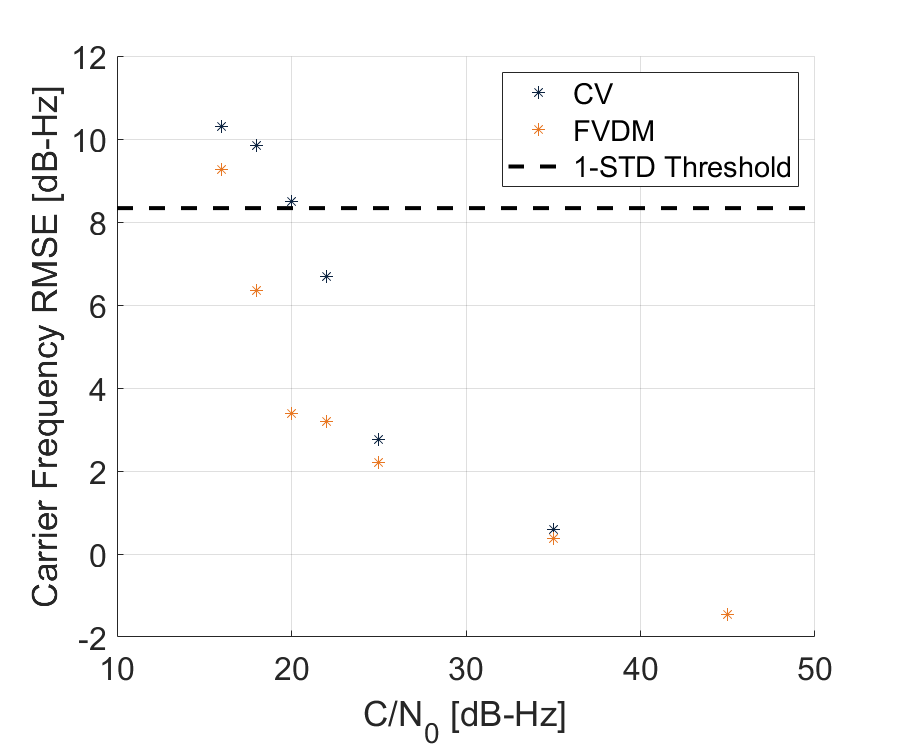
\includegraphics[width=1\linewidth]{Figures/dynamic/carrFreqRMSEdyn.png}
    \end{subfigure}
    \caption{Code phase and carrier frequency RMSE as a function of signal power, specified in dB-Hz.}\label{fig:codecarrierdyn}
\end{figure}

As previously mentioned, the excitation in the angular rates provides better observability for those estimated states along with their integrated Euler attitude counter parts. Compared to trajectory one, Figure~\ref{fig:codecarrierdyn} shows that the proposed navigation filter can track beyond \(16\) dB-Hz. Unlike the previous trajectory, even in cases of little to no interference, the deeply-coupled FVDM out performs the standard VDFLL implementation right up to benign signal power (\(45\) dB-Hz). This effective increase in performance is further shown in Figure~\ref{fig:trackingprobability2} where the probability to maintain lock across all channels is shown again for trajectory two.

\begin{figure}[!ht]
    \centering
    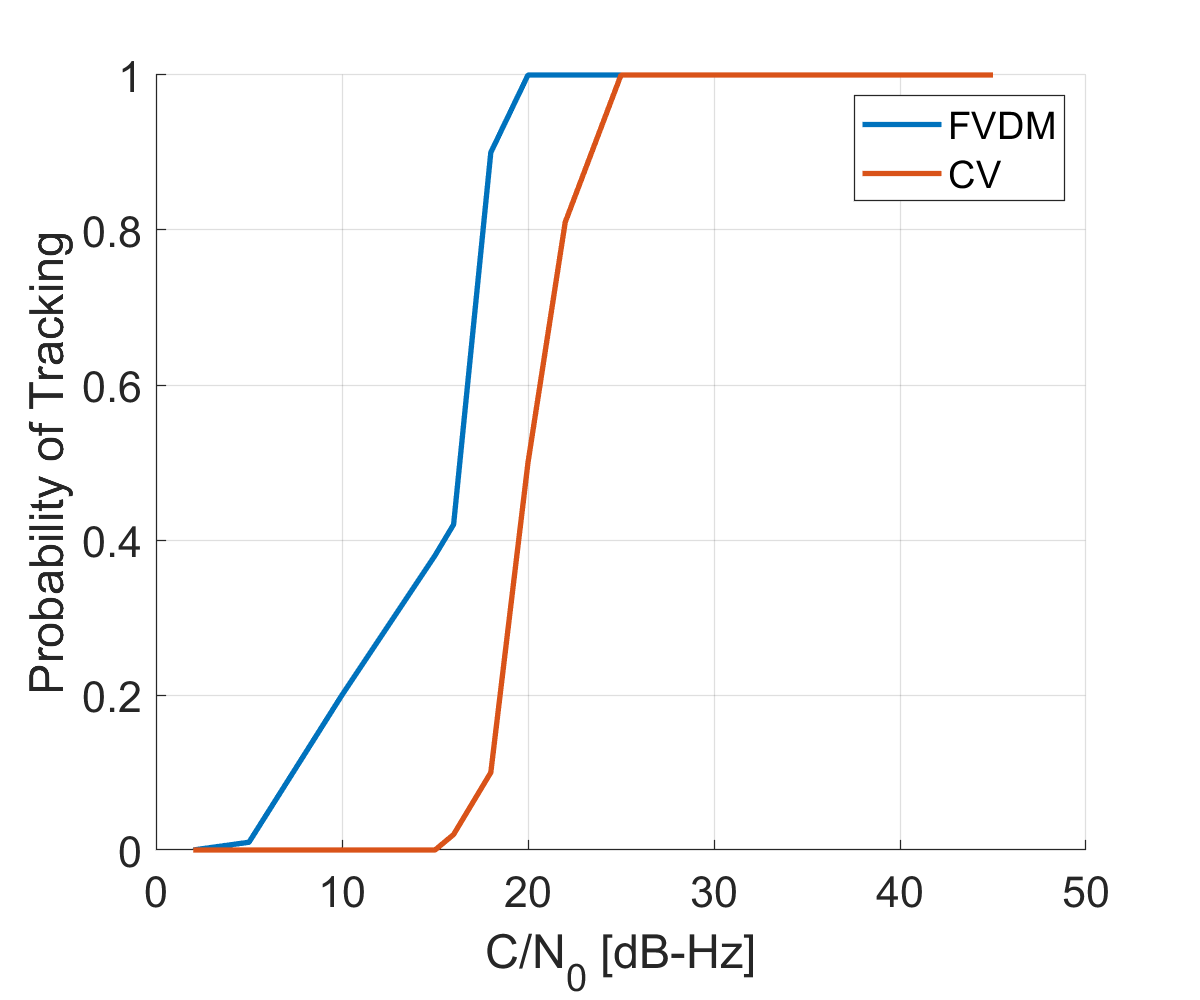
\includegraphics[width=0.5\linewidth]{Figures/dynamic/trackingprobdyn.png}
    \caption{The probability that each navigation filter is able to maintain channel lock throughout the simulation across different levels of signal interference.}\label{fig:trackingprobability2}
\end{figure}

While the deeply integrated FVDM shows approximately \(100\% \) tracking probability at the same \(20\) dB-Hz compared to Figure~\ref{fig:trackingprobability1}, the constant velocity kinematic model effectively loses lock faster after the the signal power drops below \(25\) dB-Hz. Similar to trajectory one, the same \(5\) dB-Hz improvement in tracking probability can be seen for trajectory two. The position estimates reflect the improved ability of the deeply-coupled FVDM to maintain lock in GPS-challenged environments. Figure~\ref{fig:GEOPLOT3} presents the Latitude and Longitude estimates for both filters simulated for trajectory two.

\begin{figure}[!ht]
    \begin{subfigure}{.45\textwidth}
        \centering
        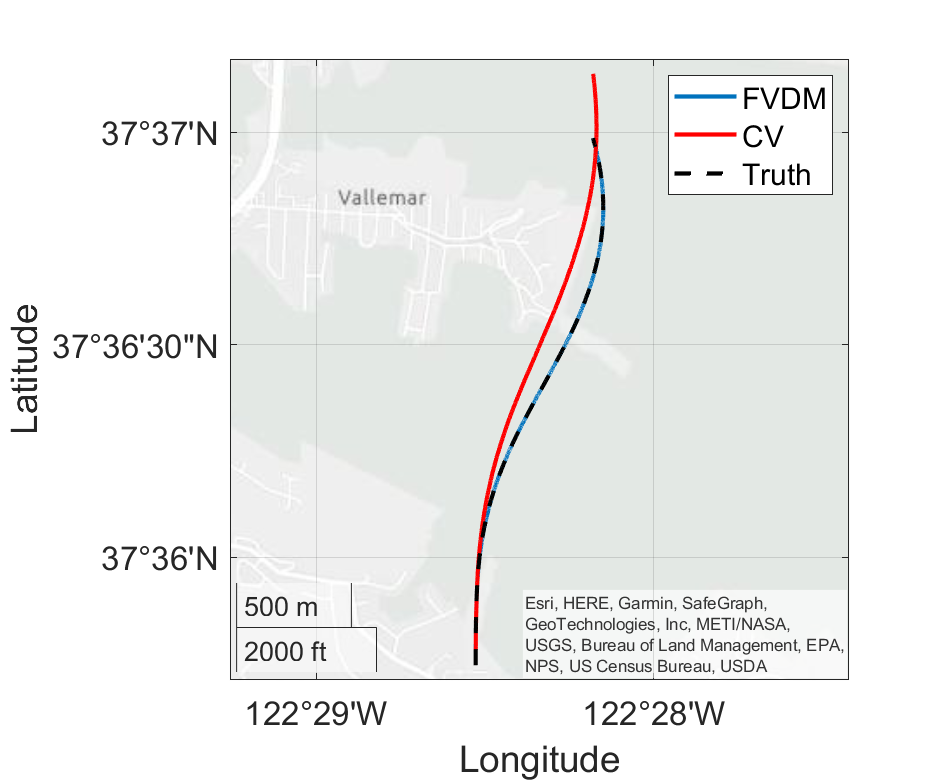
\includegraphics[width=1\linewidth]{Figures/dynamic/20/GEOPLOT.png}
    \end{subfigure}%
    \begin{subfigure}{.45\textwidth}
        \centering
        \includegraphics[width=1\linewidth]{Figures/dynamic/25/GEOPLOT.png}
    \end{subfigure}
    \caption{Average Latitude and Longitude of the FVDM and standard VDFLL implementation compared to the truth trajectory. The left figure is when both simulations had a signal power of \(20\) dB-Hz. The right figure is with a signal power of \(25\) dB-Hz.}\label{fig:GEOPLOT3}
\end{figure}

When subject to a signal power of \(20\) dB-Hz, the average Latitude and Longitude estimates for the constant velocity EKF shows a slight drift from the true location of the aircraft. Like before, this is likely due to the zero-mean acceleration assumption of the kinematic model. Furthermore, the standard VDFLL implementation is unable to predict the attitude of the aircraft, making it unable to correlate velocity and Euler attitude errors. For consistency, Figure~\ref{fig:GEOPLOT4} shows the Latitude and Longitude estimates when the receiver is subject to a signal power of \(18\) dB-Hz.

\begin{figure}[!ht]
    \centering
    \includegraphics[width=0.5\linewidth]{Figures/dynamic/18/GEOPLOT.png}
    \caption{Average Latitude and Longitude of the FVDM and standard VDFLL implementation compared to the truth trajectory when subject to a degraded signal power of \(16\) dB-Hz.}\label{fig:GEOPLOT4}
\end{figure}

At this level of interference, it is clear the constant velocity EKF faults just after initialization. With the lack of GPS correlator measurements to make corrections, the predicted location of aircraft quickly falls off target. The excited pitching motion of the aircraft brings about an improvement on the altitude estimates of the aircraft during the simulation (Figure~\ref{fig:Altitude2}).

\begin{figure}[!ht]
    \begin{subfigure}{.45\textwidth}
        \centering
        \includegraphics[width=1\linewidth]{Figures/dynamic/20/ALTITUDE.png}
    \end{subfigure}
    \begin{subfigure}{.45\textwidth}
        \centering
        \includegraphics[width=1\linewidth]{Figures/dynamic/25/ALTITUDE.png}
    \end{subfigure}
    \caption{Average altitude estimates of the FVDM and standard VDFLL implementation compared to the truth trajectory. The left figure is when both simulations had a signal power of \(20\) dB-Hz. The right figure is with a signal power of \(25\) dB-Hz.}\label{fig:Altitude2}
\end{figure}

Again, the standard VDFLL implementation shows altitude errors of roughly \(65\) meters when provided with unreliable GPS correlator measurements. The lack of diversity is to blame and adding a ground station or fusing the solution with a external sensor or FVDM would mitigate this problem. For a more detailed reference on the difference in pose estimates between the two filters, Tables~\ref{tbl:dyn20CV} and~\ref{tbl:dyn20FVDM} are included at the end of this section for further inspection. The dynamics of trajectory two prove ever more that the zero-acceleration assumption from the constant velocity kinematic model is poor. Figure~\ref{fig:Speed2} presents the speed estimates of both the proposed navigation filter and the standard VDFLL implementation subject to \(20\) and \(25\) dB-Hz of signal power.

\begin{figure}[!ht]
    \begin{subfigure}{.45\textwidth}
        \centering
        \includegraphics[width=1\linewidth]{Figures/dynamic/20/SPEED.png}
    \end{subfigure}
    \begin{subfigure}{.45\textwidth}
        \centering
        \includegraphics[width=1\linewidth]{Figures/dynamic/25/SPEED.png}
    \end{subfigure}
    \caption{Average speed estimates of the FVDM and standard VDFLL implementation compared to the truth trajectory. The left figure is when both simulations had a signal power of \(20\) dB-Hz. The right figure is with a signal power of \(25\) dB-Hz.}\label{fig:Speed2}
\end{figure}

At roughly \(10~m/s\) of error in the speed estimate (according to Table~\ref{tbl:dyn20CV}), The average drift of the estimated position presented by Figure~\ref{fig:GEOPLOT4} is understandable. It should be noted here that the throttle reference command (Chapter 5) is commanding the aircraft to keep a consistent velocity of \(70~m/s\), limitations on engine power and the advance ratio of the propeller prevent it from reaching such speeds during the climb segment. One of the primary benefits of the proposed navigation filter is the ability to estimate the angular rates and Euler attitude of the aircraft during flight. Although these states are not directly measurable by the correlator measurements, their correlation within the position and velocity equations (Equations~\ref{eq:posrate} and~\ref{eq:acc}) is substantial enough to hold accurate estimates (Figure~\ref{fig:ANGRATES}).

\begin{figure}[!ht]
    \begin{subfigure}{.45\textwidth}
        \centering
        \includegraphics[width=1\linewidth]{Figures/dynamic/15/ANGULARRATES.png}
    \end{subfigure}
    \begin{subfigure}{.45\textwidth}
        \centering
        \includegraphics[width=1\linewidth]{Figures/dynamic/20/ANGULARRATES.png}
    \end{subfigure}
    \caption{Average angular rate estimates of the FVDM and standard VDFLL implementation compared to the truth trajectory. The left figure is when both simulations had a signal power of \(15\) dB-Hz. The right figure is with a signal power of \(20\) dB-Hz.}\label{fig:ANGRATES}
\end{figure}

Although the aircraft is commanded to reach an altitude of \(1150\) meters above sea level, this does not equate to radical change in pitch rate. As seen from Figure~\ref{fig:EULER}, the aircraft reaches a steady state pitch and maintains that pitch until the altitude command is met. Since the pitch command is near-constant, unlike the roll and yaw angles, leaves the pitch rate to be near-zero for the duration of the simulation.

\begin{figure}[!ht]
    \begin{subfigure}{.45\textwidth}
        \centering
        \includegraphics[width=1\linewidth]{Figures/dynamic/15/EULERANGLES.png}
    \end{subfigure}
    \begin{subfigure}{.45\textwidth}
        \centering
        \includegraphics[width=1\linewidth]{Figures/dynamic/20/EULERANGLES.png}
    \end{subfigure}
    \caption{Average Euler attitude estimates of the FVDM and standard VDFLL implementation compared to the truth trajectory. The left figure is when both simulations had a signal power of \(15\) dB-Hz. The right figure is with a signal power of \(20\) dB-Hz.}\label{fig:EULER}
\end{figure}

Because the Euler attitude estimates are the integral of the angular rate estimate, barring the rotation of \(C_{\omega}\) (Equation~\ref{eq:eulerRates}), it is clear that worse estimates of angular rates lead to drifting error in the Euler attitude estimates of the aircraft. If not corrected, this can lead to drifting position and velocity estimation at lower \(C/N_0\) levels. To maintain better estimates of the angular rates and Euler attitude, an IMU or additional hardware sensor could be tied-in with the FVDM to provide direct measurements of those states. Another option, although sub-optimal, would be the addition of a second GPS antenna, in which GPS course measurements could be calculated and provided to the filter. It should further be noted that GPS course and the yaw of the aircraft are not the same as discussed in Chapter 2.

The clock bias and clock drift estimates from both filters are analyzed for trajectory two. Similar to trajectory one, the receiver in trajectory two is embedded with an OCXO\@. And as mentioned previously, the performance of the clock bias and drifts estimates correspond with the accuracy of the position and velocity estimates, respectively. Figure~\ref{fig:Clocks3} presents the clock bias estimates for both filters subject to the dynamics of trajectory two and signal power degradation. Figure~\ref{fig:Clocks4} dictates the clock drifts estimates under the same circumstances.


\begin{figure}[!ht]
    \begin{subfigure}{.45\textwidth}
        \centering
        \includegraphics[width=1\linewidth]{Figures/dynamic/25/CLOCKBIAS.png}
    \end{subfigure}
    \begin{subfigure}{.45\textwidth}
        \centering
        \includegraphics[width=1\linewidth]{Figures/dynamic/35/CLOCKBIAS.png}
    \end{subfigure}
    \caption{Average clock bias estimates of the FVDM and standard VDFLL implementation compared to the truth trajectory. The left figure is when both simulations had a signal power of \(20\) dB-Hz. The right figure is with a signal power of \(25\) dB-Hz.}\label{fig:Clocks3}
\end{figure}

\begin{figure}[!ht]
    \begin{subfigure}{.45\textwidth}
        \centering
        \includegraphics[width=1\linewidth]{Figures/dynamic/25/CLOCKDRIFT.png}
    \end{subfigure}
    \begin{subfigure}{.45\textwidth}
        \centering
        \includegraphics[width=1\linewidth]{Figures/dynamic/35/CLOCKDRIFT.png}
    \end{subfigure}
    \caption{Average clock drift estimates of the FVDM and standard VDFLL implementation compared to the truth trajectory. The left figure is when both simulations had a signal power of \(20\) dB-Hz. The right figure is with a signal power of \(25\) dB-Hz.}\label{fig:Clocks4}
\end{figure}

Lastly, Tables~\ref{tbl:dyn20FVDM} and~\ref{tbl:dyn20CV} provide the RMSE, STD, and maximum error calculated across the 100-run Monte Carlo simulation when the receiver is subject to interference that leaves the signal power at \(20\) dB-Hz.
\begin{table}[!ht]
    \caption{RMSE, STD, and maximum error from 100-run Monte Carlo simulation when the receiver is subject to a degraded signal power level of \(20\) dB-Hz.}\label{tbl:dyn20FVDM}
    \centering
    \begin{tabular}{ccccc}
        \toprule
                  & Position [m] & Speed [m/s] & Clock Bias [m] & Clock Drift [m/s] \\
        \midrule
        RMSE      & 0.64521      & 0.2673      & 0.1911         & 0.010044          \\
        STD       & 0.34121      & 0.12531     & 0.18278        & 0.0073514         \\
        Max Error & 1.5828       & 0.76501     & 0.5855         & 0.23049           \\
        \bottomrule
    \end{tabular}
\end{table}

\begin{table}[!ht]
    \caption{RMSE, STD, and maximum error from 100-run Monte Carlo simulation when the receiver is subject to a degraded signal power level of \(20\) dB-Hz.}\label{tbl:dyn20CV}
    \centering
    \begin{tabular}{ccccc}
        \toprule
                  & Position [m] & Speed [m/s] & Clock Bias [m] & Clock Drift [m/s] \\
        \midrule
        RMSE      & 196.98       & 6.0576      & 0.20098        & 0.010995          \\
        STD       & 126.68       & 0.92248     & 0.19358        & 0.0077631         \\
        Max Error & 431.72       & 8.468       & 0.62891        & 0.024964          \\
        \bottomrule
    \end{tabular}
\end{table}

% \begin{table}[!ht]
%     \caption{RMSE, STD, and maximum error from 100-run Monte Carlo simulation when the receiver is subject to a degraded signal power level of \(35\) dB-Hz.}\label{tbl:dyn35FVDM}
%     \centering
%     \begin{tabular}{ccccc}
%         \toprule
%                   & Position [m] & Speed [m/s] & Clock Bias [m] & Clock Drift [m/s] \\
%         \midrule
%         RMSE      & 0.023097     & 0.068845    & 0.028182       & 0.0026012         \\
%         STD       & 0.12219      & 0.03264     & 0.021298       & 0.0029319         \\
%         Max Error & 0.74388      & 0.28942     & 0.073095       & 0.008722          \\
%         \bottomrule
%     \end{tabular}
% \end{table}

% \begin{table}[!ht]
%     \caption{RMSE, STD, and maximum error from 100-run Monte Carlo simulation when the receiver is subject to a degraded signal power level of \(35\) dB-Hz.}\label{tbl:dyn35CV}
%     \centering
%     \begin{tabular}{ccccc}
%         \toprule
%                   & Position [m] & Speed [m/s] & Clock Bias [m] & Clock Drift [m/s] \\
%         \midrule
%         RMSE      & 0.097444     & 0.080918    & 0.030903       & 0.0033113         \\
%         STD       & 0.031969     & 0.035597    & 0.02659        & 0.0039156         \\
%         Max Error & 0.1905       & 0.23272     & 0.076362       & 0.00917           \\
%         \bottomrule
%     \end{tabular}
% \end{table}


\section{\textbf{Conclusions}}

This chapter presented a detailed explanation of the two trajectories used for the performance analysis of the proposed navigation filter compared to a standard, constant-velocity kinematic model VDFLL\@. Trajectory one is the baseline case where the aircraft is commanded to fly straight and maintain a constant altitude for the entirety of the simulation. Trajectory two is a more dynamic trajectory with alternating, banking turns throughout the simulation on top of the aircraft being commanded to climb and maintain an altitude of 1150 meters. Each trajectory was subject to a range of interferences starting from benign signal power to low signal power. Results from trajectory one show that when flying a standard, unexcited trajectory, the standard VDFLL and the proposed navigation filter are comparable. Results from trajectory two showcase the improved performance from the deeply-coupled FVDM because of the inability in the standard EKF to predict angular rates and Euler attitude. However, the results from trajectory two also show that the FVDM is not the sole-solution due to the unobservable angular states when excitement is lost in the simulated trajectory. External sensors such as a IMU or multi-antenna GPS system could improve the system observability for better estimates. Improvements to the proposed navigation filter are discussed in greater details in the next chapter.
\chapter{Conclusion and Future Work}
This work described the development of a deeply-integrated flight vehicle dynamic model within a GPS L1 C/A vector tracking software defined receiver. Furthermore, a performance analysis of the proposed navigation filter in GPS-challenged environments was presented. The work presented in this thesis extends the state of the art by modeling a vehicle dynamic model deeply-coupled with GPS measurements. A model of the Diamond DA-40 is presented. The fidelity of the model stems from multiple flight mechanic modules presented in Chapter 2. The aerodynamic module models aerodynamic forces and moments on the basis of strip theory, using pre-processed CFD tables to propagate the aerodynamic coefficients based on the current orientation of the flight vehicle. The engine and propeller module comprise of pre-processed numerical tables based on engine and propeller knowledge within the Diamond DA-40. The third module is the landing-gear, modeled after a second-order mass-spring-damper ordinary differential equation. The FVDM benefits the extended Kalman filter by fully acknowledging the behavior of the presented flight vehicle {--} this can be cumbersome with hardware sensors such as an IMU or barometer working alone. The presented FVDM can be run at any update frequency, typically a limiting factor for hardware sensors. An increased update frequency for any vehicle dynamic model increases the likelihood that changes in the states between updates are linear, this is especially important for high-dynamic systems such as hyper-velocity vehicles. Unlike hardware sensors, the FVDM is not subject to vibration, which is a common amongst rotor craft and fixed-wing flight vehicles. The downside to the FVDM is lack of observability when propagating the states of the flight vehicle in the local navigation frame. The FVDM presented in this work is also agnostic to the current atmospheric conditions, which could degrade vehicle pose estimation. However, this can be improved upon and is discussed later in this chapter.

In benign conditions, the fusion of the FVDM with GPS correlator-level measurements shows improvements over tightly and loosely-coupled architectures found in the literature. The effective carrier-to-noise ratio benefit from the vector tracking SDR improves estimation performance in GPS degraded environments, but the lack of observability in the angular rates and Euler angles severely inhibits the performance of the proposed navigation filter in GPS-denied scenarios.
\section{\textbf{Concerns of Observability}}

From the presented navigation filter, measurements of position and velocity appear in the form of pseudorange and pseudorange-rates. These measurements are created based on DLL and FLL discriminator outputs that are converted to meters and meters per second, respectively. When a measurement update occurs within the EKF, these measurements indirectly correct the current state estimate through a the observation matrix, \(\mathbf{H}\) (Equation~\ref{eq:H}). As stated previously, one reason for faulty estimates of the aircraft in GPS-denied environments is the lack of observability in the angular states. Once the estimated angular rates of the aircraft drift, and through integration, their respective Euler angles, the FVDM will continue to propagate the aircraft with these drifting estimates. For example, if the pitch angle estimate of the FVDM starts to drift from 10 degrees to 20 degrees to 30 degrees, the aircraft will naturally begin to pitch up and gain altitude. If the VT algorithm loses lock with signal channels, or the channel measurements are poor, there is no other measurements to correct the FVDM and it will continue to propagate worse estimates of the state. This can be further examined by exploring the observability matrix, \(\mathbf{O}\) through time.

\begin{equation}\label{eq:O}
    \mathbf{O} = \begin{bmatrix}
        \mathbf{H}_k                    \\
        \mathbf{H}_k\mathbf{\Phi}_k       \\
        \mathbf{H}_k\mathbf{\Phi}_k^2     \\
        \mathbf{H}_k\mathbf{\Phi}_k^3     \\
        \vdots                        \\
        \mathbf{H}_k\mathbf{\Phi}_k^{n-1} \\
    \end{bmatrix}
\end{equation}

A system is fully-observable if the all of the states of the system can be known by the outputs of the systems, that is, if the rank of Equation~\ref{eq:O} is equal to the number of states in \(\mathbf{X}\) (Equation~\ref{eq:stateVector}), then the observability matrix is full rank and the system is fully-observable. A quick calculation of \(\mathbf{O}\) shows that the deeply-coupled FVDM is not fully-observable. 


\section{\textbf{Future Work}}
For future work, the author recommends several items, both relating to the proposed navigation filter and to components of the FVDM presented in this work. In addition to the deeply-coupled FVDM with GPS correlator measurements, a recommendation is made to couple IMU or other external sensors with the FVDM for improvement in observability of angular rates and Euler angles. The addition of an IMU would provide a direct measurement of angular rates and specific forces that would correct the predicted forces and moments from the FVDM\@. This is especially beneficial in GPS-denied environments. The addition of a barometer would provide a direct measurement of pressure, which could be mapped to the altitude of the FVDM\@. The direct measurement of altitude would correct the FVDM in GPS-denied environments, and subsequently could provide an semi-observable mapping to pitch, pitch-rate, and the climb rate (\(V_D\)) of the FVDM\@. These recommendations stem from prior work performed by~\cite{khaghaniAssessmentVDMbasedAutonomous2018,khaghaniAutonomousVehicleDynamic2016,mwenegohaModelbasedTightlyCoupled2020} for loosely and tightly coupled architectures. In reality, flying on any given day will not have standard-day atmospheric conditions as modeled for this work.  To better match actual atmospheric conditions, an implementation of a non-standard day atmospheric model is recommended. A comparative analysis of FVDM performance between the two atmospheric models is intriguing and is also recommended. For improvements to the vector tracking architecture, the author recommends implementation of a multi-signal vector tracking algorithm as seen in~\cite{givhanGPSL5Software2021}. The addition of another signal from a different constellation would increase the number of measurements greatly (especially if using a low-Earth orbit constellation). With modern signal modulation, the resistance to interference is increased, allowing vector tracking to retain channel lock even in scenarios of heavy degradation.

\printbibliography{}


\appendix
\chapter*{Appendix A\\ Extra Results from Scenario 1\addcontentsline{toc}{chapter}{Appendices}}
\addcontentsline{toc}{section}{Appendix A {--} Extra Results from Scenario 1}

\begin{figure}[!ht]
  \centering
  \includegraphics[width=0.75\linewidth]{Figures/Results/trajectoryfigure/Slide16.PNG}
  \caption{Clock bias and Clock drift estimates using the proposed navigation filter when subject to instantaneous interference, bringing the \(C/N_0\) to \(25\) dB-Hz.}\label{fig:PosVel25}
\end{figure}


\begin{figure}[!ht]
  \centering
  \includegraphics[width=0.75\linewidth]{Figures/Results/trajectoryfigure/Slide4.PNG}
  \caption{Clock bias and Clock drift estimates using the proposed navigation filter when subject to instantaneous interference, bringing the \(C/N_0\) to \(25\) dB-Hz.}\label{fig:Eul25}
\end{figure}


\begin{figure}[!ht]
  \centering
  \includegraphics[width=0.75\linewidth]{Figures/Results/trajectoryfigure/Slide10.PNG}
  \caption{Clock bias and Clock drift estimates using the proposed navigation filter when subject to instantaneous interference, bringing the \(C/N_0\) to \(25\) dB-Hz.}\label{fig:Ang25}
\end{figure}


\begin{figure}[!ht]
  \centering
  \includegraphics[width=0.75\linewidth]{Figures/Results/trajectoryfigure/Slide22.PNG}
  \caption{Clock bias and Clock drift estimates using the proposed navigation filter when subject to instantaneous interference, bringing the \(C/N_0\) to \(25\) dB-Hz.}\label{fig:Clk25}
\end{figure}

\begin{figure}[!ht]
  \centering
  \includegraphics[width=0.75\linewidth]{Figures/Results/trajectoryfigure/Slide17.PNG}
  \caption{Clock bias and Clock drift estimates using the proposed navigation filter when subject to instantaneous interference, bringing the \(C/N_0\) to \(30\) dB-Hz.}\label{fig:PosVel30}
\end{figure}


\begin{figure}[!ht]
  \centering
  \includegraphics[width=0.75\linewidth]{Figures/Results/trajectoryfigure/Slide5.PNG}
  \caption{Clock bias and Clock drift estimates using the proposed navigation filter when subject to instantaneous interference, bringing the \(C/N_0\) to \(30\) dB-Hz.}\label{fig:Eul30}
\end{figure}


\begin{figure}[!ht]
  \centering
  \includegraphics[width=0.75\linewidth]{Figures/Results/trajectoryfigure/Slide11.PNG}
  \caption{Clock bias and Clock drift estimates using the proposed navigation filter when subject to instantaneous interference, bringing the \(C/N_0\) to \(30\) dB-Hz.}\label{fig:Ang30}
\end{figure}


\begin{figure}[!ht]
  \centering
  \includegraphics[width=0.75\linewidth]{Figures/Results/trajectoryfigure/Slide23.PNG}
  \caption{Clock bias and Clock drift estimates using the proposed navigation filter when subject to instantaneous interference, bringing the \(C/N_0\) to \(30\) dB-Hz.}\label{fig:Clk30}
\end{figure}

\begin{figure}[!ht]
  \centering
  \includegraphics[width=0.75\linewidth]{Figures/Results/trajectoryfigure/Slide18.PNG}
  \caption{Clock bias and Clock drift estimates using the proposed navigation filter when subject to instantaneous interference, bringing the \(C/N_0\) to \(35\) dB-Hz.}\label{fig:PosVel35}
\end{figure}


\begin{figure}[!ht]
  \centering
  \includegraphics[width=0.75\linewidth]{Figures/Results/trajectoryfigure/Slide6.PNG}
  \caption{Clock bias and Clock drift estimates using the proposed navigation filter when subject to instantaneous interference, bringing the \(C/N_0\) to \(35\) dB-Hz.}\label{fig:Eul35}
\end{figure}


\begin{figure}[!ht]
  \centering
  \includegraphics[width=0.75\linewidth]{Figures/Results/trajectoryfigure/Slide12.PNG}
  \caption{Clock bias and Clock drift estimates using the proposed navigation filter when subject to instantaneous interference, bringing the \(C/N_0\) to \(35\) dB-Hz.}\label{fig:Ang35}
\end{figure}


\begin{figure}[!ht]
  \centering
  \includegraphics[width=0.75\linewidth]{Figures/Results/trajectoryfigure/Slide24.PNG}
  \caption{Clock bias and Clock drift estimates using the proposed navigation filter when subject to instantaneous interference, bringing the \(C/N_0\) to \(35\) dB-Hz.}\label{fig:Clk35}
\end{figure}



\end{document}

